\documentclass{article}

% NeurIPS 2026 submission style.
% This paper targets the Evaluations & Datasets track.  For camera-ready,
% switch to \usepackage[eandd, final]{neurips_2026}.
\usepackage[eandd]{neurips_2026}

\usepackage[utf8]{inputenc}
\usepackage[T1]{fontenc}
\usepackage[hypertexnames=false]{hyperref}
\usepackage{url}
\usepackage{booktabs}
\usepackage{amsfonts}
\usepackage{amsmath}
\usepackage{amssymb}
\usepackage{nicefrac}
\usepackage{microtype}
\usepackage{xcolor}
\usepackage{graphicx}
\usepackage{array}
\usepackage{longtable}
\usepackage{multirow}
\usepackage{enumitem}
\usepackage{algorithm}
\usepackage{algpseudocode}
\usepackage{cleveref}

\title{SymbolicArena: A Unified Infrastructure for Benchmark Distillation and Dynamic Evaluation in Symbolic Regression}

\author{%
  Anonymous Authors \\
  Anonymous Institution \\
  \texttt{anonymous@anonymous.org}
}

\newcommand{\arena}{\textbf{SymbolicArena}}
\newcommand{\core}{Core-50}
\newcommand{\reservoir}{GT-Reservoir-664}
\newcommand{\candidate}{Candidate-200}
\newcommand{\probe}{Probe-4}
\newcommand{\idq}{\textsc{ID-Q}}
\newcommand{\oodg}{\textsc{OOD-G}}
\newcommand{\symf}{\textsc{SYM-F}}
\newcommand{\eff}{\textsc{EFF}}
\newcommand{\rob}{\textsc{ROBU}}
\newcommand{\stab}{\textsc{STAB}}

\begin{document}

\maketitle

\begin{abstract}
%Symbolic regression (SR) is rapidly diversifying across evolutionary, reinforcement-learning, tree-search, neural-guided, and LLM-assisted paradigms, yet current evaluation remains fragmented across heterogeneous benchmarks, execution protocols, and task scales. This makes it difficult to obtain reliable feedback during algorithm development or to compare methods beyond final numerical error. We introduce \arena{}, a unified infrastructure for benchmark distillation and dynamic evaluation in symbolic regression. \arena{} starts from a large pool of candidate tasks, constructs a 664-task ground-truth reservoir, integrates 12 representative SR algorithms, and distills the reservoir into a fixed \core{} benchmark through cascaded probe-based selection. The selection jointly accounts for task-structure coverage, algorithmic response diversity, method discriminability, semantic redundancy, difficulty balance, and seed-level stability, allowing \core{} to retain the main characteristics of the full reservoir at substantially lower evaluation cost. Beyond benchmark distillation, \arena{} provides a dynamic leaderboard: 12 algorithms are evaluated on \core{} with five seeds under a unified one-hour budget, while best-so-far expressions are logged every minute and canonicalized into a shared symbolic representation. This yields 3,000 clean leaderboard runs and 180,000 expression snapshots. We further define a fixed absolute 0--100 hexagonal protocol with five clean-track axes covering ID numerical quality, OOD generalization, symbolic fidelity, efficiency, and effective stability, plus a standardized noisy-training robustness extension. In total, \arena{} connects dataset standardization, benchmark compression, unified algorithm execution, expression-level tracing, and multi-axis evaluation into a reproducible and extensible evaluation substrate for modern SR research.

Symbolic regression (SR) is rapidly diversifying across evolutionary, reinforcement-learning, tree-search, neural-guided, transformer-based, and LLM-assisted paradigms, while evaluation remains fragmented across heterogeneous benchmarks and protocols. \arena{}, a unified infrastructure for benchmark distillation and dynamic SR evaluation, is introduced. Starting from nearly one thousand candidate tasks, \arena{} constructs a 664-task quality-checked ground-truth reservoir, integrates 12 representative algorithms, and distills a fixed \core{} benchmark through cascaded probe-based selection. The selection preserves task-structure coverage, algorithmic response diversity, method discriminability, redundancy control, difficulty balance, and seed-level stability at substantially lower evaluation cost. \arena{} further evaluates algorithms under a unified one-hour protocol with standardized artifacts, failure semantics, expression canonicalization, and minute-level best-so-far logging. A fixed absolute 0--100 hexagonal protocol covers in-distribution (ID) numerical quality, out-of-distribution (OOD) generalization,, symbolic fidelity, efficiency, stability, and noisy-training robustness. Supported by nearly 30,000 runs, \arena{} provides a reproducible and extensible evaluation substrate for modern SR research.
\end{abstract}

\section{Introduction}

Symbolic regression (SR) aims to discover compact and interpretable mathematical expressions from data, making it a central tool for scientific modeling and equation discovery. While early and widely used SR systems were largely built around genetic programming and evolutionary search \citep{koza1992genetic,cranmer2023pysr}, recent methods span reinforcement learning and policy search \citep{petersen2021dsr}, modular neural-guided search \citep{landajuela2022unified}, Monte Carlo tree search and planning \citep{kamienny2023deep,shojaee2023tpsr}, transformer-based expression generation \citep{valipour2021symbolicgpt}, and LLM-assisted scientific equation discovery \citep{shojaee2025llmsr,grayeli2024lasr}. This diversity is scientifically valuable, yet it also reshapes the benchmark problem by requiring SR methods to be evaluated along multiple dimensions, including numerical accuracy, symbolic recovery, out-of-distribution generalization and seed stability.

Existing SR benchmarks provide important foundations for reproducible comparison \citep{lacava2021contemporary,matsubara2024rethinking,shojaee2025llmsrbench,xu2024geobench}. SRBench\citep{lacava2021contemporary} established a living benchmark for comparing contemporary SR methods across real-world and synthetic regression problems ; SRSD\citep{matsubara2024rethinking} revisited equation-discovery datasets with carefully designed sampling ranges, dummy variables, and expression-level similarity metrics; recent benchmarks such as LLM-SRBench\citep{shojaee2025llmsrbench} and GeoBench\citep{xu2024geobench} further target LLM-based scientific discovery and domain-specific symbolic reasoning. However, they are difficult to use as a fast, stable, and fine-grained evaluation substrate for the current algorithmic landscape. Large benchmark suites are expensive to run during iterative method development, while smaller suites can be redundant, biased toward particular formula families, or unable to preserve conclusions from a larger task pool. Static leaderboards further limit evaluation by collapsing algorithmic behavior into final aggregate scores, thereby obscuring search trajectories, invalid outputs, expression complexity, and failure modes that are central to judging practical SR utility.

We argue that a modern SR benchmark should function as evaluation infrastructure rather as a static dataset collection. It should provide reliable comparison across heterogeneous tasks, algorithms, and future submissions. %Therefore, \arena{} is designed around four principles: executable dataset standardization, compact reservoir-preserving benchmark distillation, unified algorithm execution with comparable artifacts, and an absolute dynamic leaderboard whose scores remain interpretable as new methods are added. This design enables SR evaluation to capture both final performance and algorithmic behavior, including ID/OOD accuracy, symbolic recovery, failures, complexity, and search dynamics.
%
To address these challenges, \arena{}, a standardized evaluation infrastructure for symbolic regression is proposed. It starts from nearly one thousand candidate tasks and constructs a 664-task ground-truth reservoir with standardized schemas%, executable programs, canonical expressions, ID/OOD splits, and task metadata
. A compact \core{} benchmark is distilled from the 664-task reservoir through a cascaded probe-based selection pipeline. Rather than relying on a single difficulty heuristic or manual preference, \core{} is selected by jointly optimizing task-structure coverage, response diversity, method discriminability, difficulty and failure-mode balance. 

Moreover, \arena{} introduces a fixed six-axis evaluation protocol for dynamic SR leaderboards, covering in-distribution numerical quality, out-of-distribution generalization, symbolic fidelity, efficiency cost, noise robustness, and effective stability. Combined with best-so-far search traces, this protocol supports stable long-term algorithm comparison and fine-grained analysis of SR search behavior. Empirically, we assess whether the distilled \core{} better preserves reservoir-level conclusions than common subset-selection baselines, and use the resulting leaderboard to analyze trade-offs among numerical accuracy, symbolic recovery, OOD generalization, efficiency, robustness, and stability.

Our contributions can be summarized as follows:
\begin{itemize}[leftmargin=*, itemsep=2pt, topsep=2pt, parsep=0pt]
    \item \textbf{Unified SR evaluation stack.}
    \arena{} standardizes datasets, wrappers, budgets, failure handling, expression normalization, artifacts, and minute-level logs for fair comparison across 12 SR algorithms.

    \item \textbf{Cascaded Core-50 distillation.}
    From 664 ground-truth tasks, \arena{} constructs \core{} through dual-probe mining, 12-algorithm calibration, \probe{} selection, and multi-seed reservoir probing.

    \item \textbf{Validated compact benchmark.}
    \core{} is designed to preserve coverage, diversity, discriminability, stability, difficulty balance, and low redundancy, and is validated against repeated subset-selection baselines.

    \item \textbf{Maintainable dynamic leaderboard.}
    \arena{} reports fixed-formula scores for \idq{}, \oodg{}, \symf{}, \eff{}, and \stab{}, with \rob{} as a noisy-training extension, enabling leaderboard expansion without score drift.
\end{itemize}

%The clean evaluation pipeline comprises 14,696 runs: 1,328 dual-probe runs, 2,400 \candidate{} calibration runs, 7,968 \probe{} full-reservoir runs, and 3,000 \core{} leaderboard runs. The leaderboard stage additionally produces 180,000 best-so-far expression snapshots; the optional noisy-training robustness track adds 9,000 runs. The central claim is not that 50 tasks can replace all SR evaluation. Rather, \core{} is designed as a high-information, low-cost, reproducible core benchmark that retains the main characteristics of a much larger SR task reservoir while supporting fast and extensible leaderboard updates.

% \section{Positioning}

\paragraph{SR benchmarks.}
SRBench, SRSD, and LLM-SRBench provide the closest benchmark context for this work \citep{lacava2021contemporary,matsubara2024rethinking,shojaee2025llmsrbench}. They establish large task pools, formula-backed scientific-discovery settings, and LLM-oriented equation-discovery tests. \arena{} uses these resources as sources and reference points, but addresses a different question: how to turn a heterogeneous reservoir into a compact benchmark and dynamic leaderboard whose construction, failures, and scores remain auditable as new algorithms are added.

\paragraph{Modern SR algorithms.}
Current SR methods span evolutionary search, RL and neural-guided program generation, tree search, transformers, and LLM-assisted systems \citep{cranmer2023pysr,petersen2021dsr,landajuela2022unified,shojaee2023tpsr,shojaee2025llmsr}. These paradigms differ in their search spaces, priors, constant fitting, output validity, and sensitivity to prompt or pretrained-model distributions. \arena{} is therefore not designed around one solver family; its execution layer standardizes these methods into one result schema while preserving algorithm-specific failure semantics.

\paragraph{Benchmark distillation and dynamic evaluation.}
Efficient evaluation work such as tinyBenchmarks and SubLIME shows that smaller subsets can preserve conclusions from larger benchmark suites when subset selection is explicitly validated \citep{polo2024tinybenchmarks,saranathan2025sublime}. Dynamic evaluation systems such as Dynabench, Dynaboard, and DataPerf emphasize benchmark maintenance and score comparability over time \citep{kiela2021dynabench,ma2021dynaboard,mazumder2023dataperf}. \arena{} adapts these ideas to formula-backed SR by combining probe-based task distillation, expression-level traces, and fixed absolute scores. A fuller related-work discussion is provided in \cref{app:related-work}.

% %\section{\arena{} Overview}
% %\arena{} is organized around the evaluation loop summarized in \cref{fig:symbolicarena-pipeline}: standardize a large SR task reservoir, select a compact high-information core, execute diverse algorithms under a shared contract, and update a dynamic leaderboard from comparable artifacts.
% \begin{figure}[H]
% \centering
% 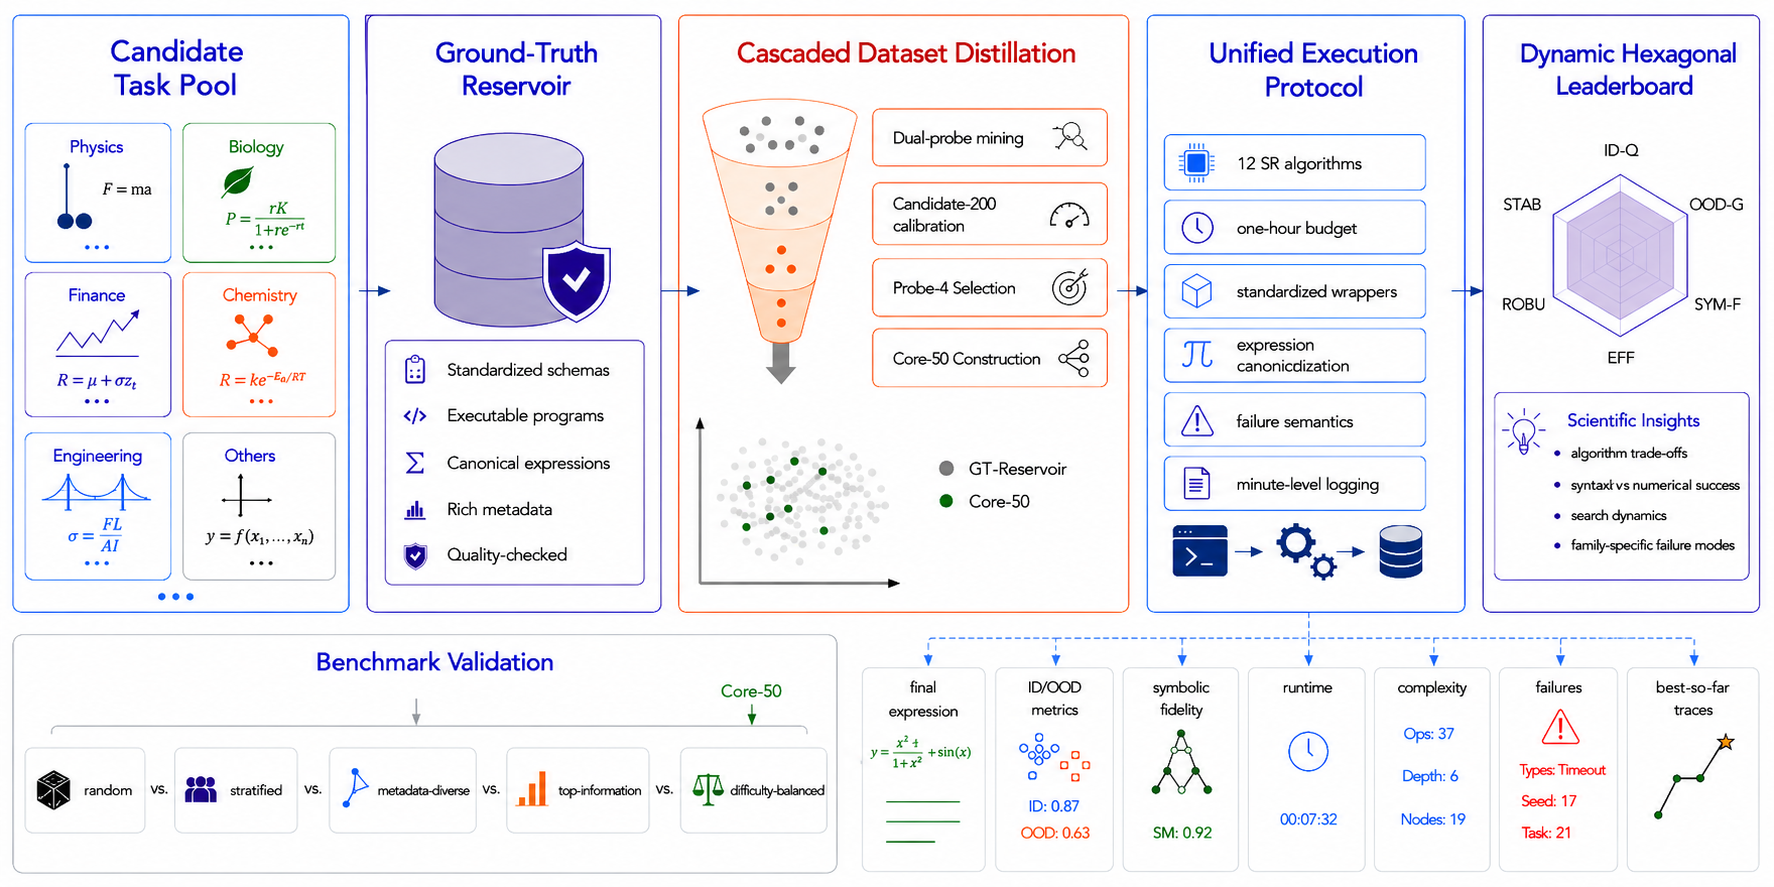
\includegraphics[width=\linewidth]{imgs/Article/figure01_pipeline}
% \caption{\textbf{Overview of \arena{}}. A heterogeneous symbolic regression task pool is standardized into a quality-checked ground-truth reservoir, then a compact and high-information Core-50 benchmark is distilled through cascaded dataset selection. It is evaluated under a unified execution protocol to produce a dynamic six-axis leaderboard and fine-grained search traces. }
% \label{fig:symbolicarena-pipeline}
% \end{figure}


% %
% %\paragraph{Dataset reservoir.}
% %The dataset layer converts heterogeneous SR sources into a shared executable format. Each task has train, validation, ID test, and OOD test splits when available, a ground-truth expression, metadata for structural analysis, and a canonical identity used for semantic duplicate control. This layer is essential because benchmark compression is only meaningful when the larger pool is itself auditable and consistently runnable.
% %
% %\paragraph{Algorithm panel.}
% The algorithm layer integrates 12 representative SR methods across evolutionary, reinforcement-learning, tree-search, neural-guided, transformer, and LLM-assisted families. Every wrapper receives the same data contract, including feature names, target names, dimensionality, budget, seed, and output path. Each run writes a canonical result artifact with status, failure reason, expression, numerical metrics, complexity, runtime, and progress snapshots when available.

% \paragraph{Execution infrastructure.}
% \arena{} uses a layered execution design rather than calling algorithm repositories directly from the benchmark script. A lightweight front-end regressor resolves the requested tool, launches the corresponding wrapper in its configured conda environment, and communicates through JSON commands. The benchmark runner is responsible for loading standardized datasets, injecting the explicit data contract, applying the shared budget and seed, computing train/validation/ID/OOD metrics, exporting canonical symbolic artifacts, and writing result and progress files. This design isolates incompatible dependencies while keeping the result schema and failure semantics identical across methods; implementation details for the execution stack, wrapper contract, result-recovery logic, and data-cleaning pipeline are provided in \cref{app:infra-cleaning}.

% \paragraph{\core{} distillation engine.}
% The distillation layer separates two roles that are often conflated in benchmark construction. The first role is \emph{candidate discovery}: identifying tasks that expose informative method differences. \arena{} performs this with PySR and LLM-SR as two complementary single-seed probes. The second role is \emph{core selection}: choosing a compact benchmark whose structure and response patterns remain representative of the full reservoir. \arena{} performs this with four non-LLM probes selected from the 12-algorithm calibration panel, then runs them on the full 664-task reservoir with three seeds.

% \paragraph{Dynamic leaderboard engine.}
% The leaderboard layer evaluates submitted algorithms on \core{} under a fixed one-hour budget and five seeds. Unlike static final-score tables, \arena{} stores best-so-far expressions at minute resolution. This makes it possible to compare algorithms by final quality, anytime efficiency, symbolic recovery, complexity growth, robustness, and seed stability. Since the six leaderboard axes are normalized against fixed absolute definitions rather than the current set of competitors, adding a new algorithm does not change the previously reported scores.

% \paragraph{Design principle.}
% \arena{} is deliberately not optimized to make all methods win equally. Its goal is to preserve informative differences among methods while keeping the evaluation cost low enough for repeated use. This leads to a benchmark design that balances coverage, discriminability, redundancy control, difficulty, and stability, instead of selecting only the largest-gap or easiest-to-run tasks.
\section{\arena{} Overview}

\arena{} is organized around the evaluation loop summarized in \cref{fig:symbolicarena-pipeline}: a heterogeneous SR task pool is standardized into an auditable ground-truth reservoir, distilled into a compact Core-50 benchmark, evaluated under a unified execution protocol, and reported through a dynamic six-axis leaderboard.

\begin{figure}[t]
\centering
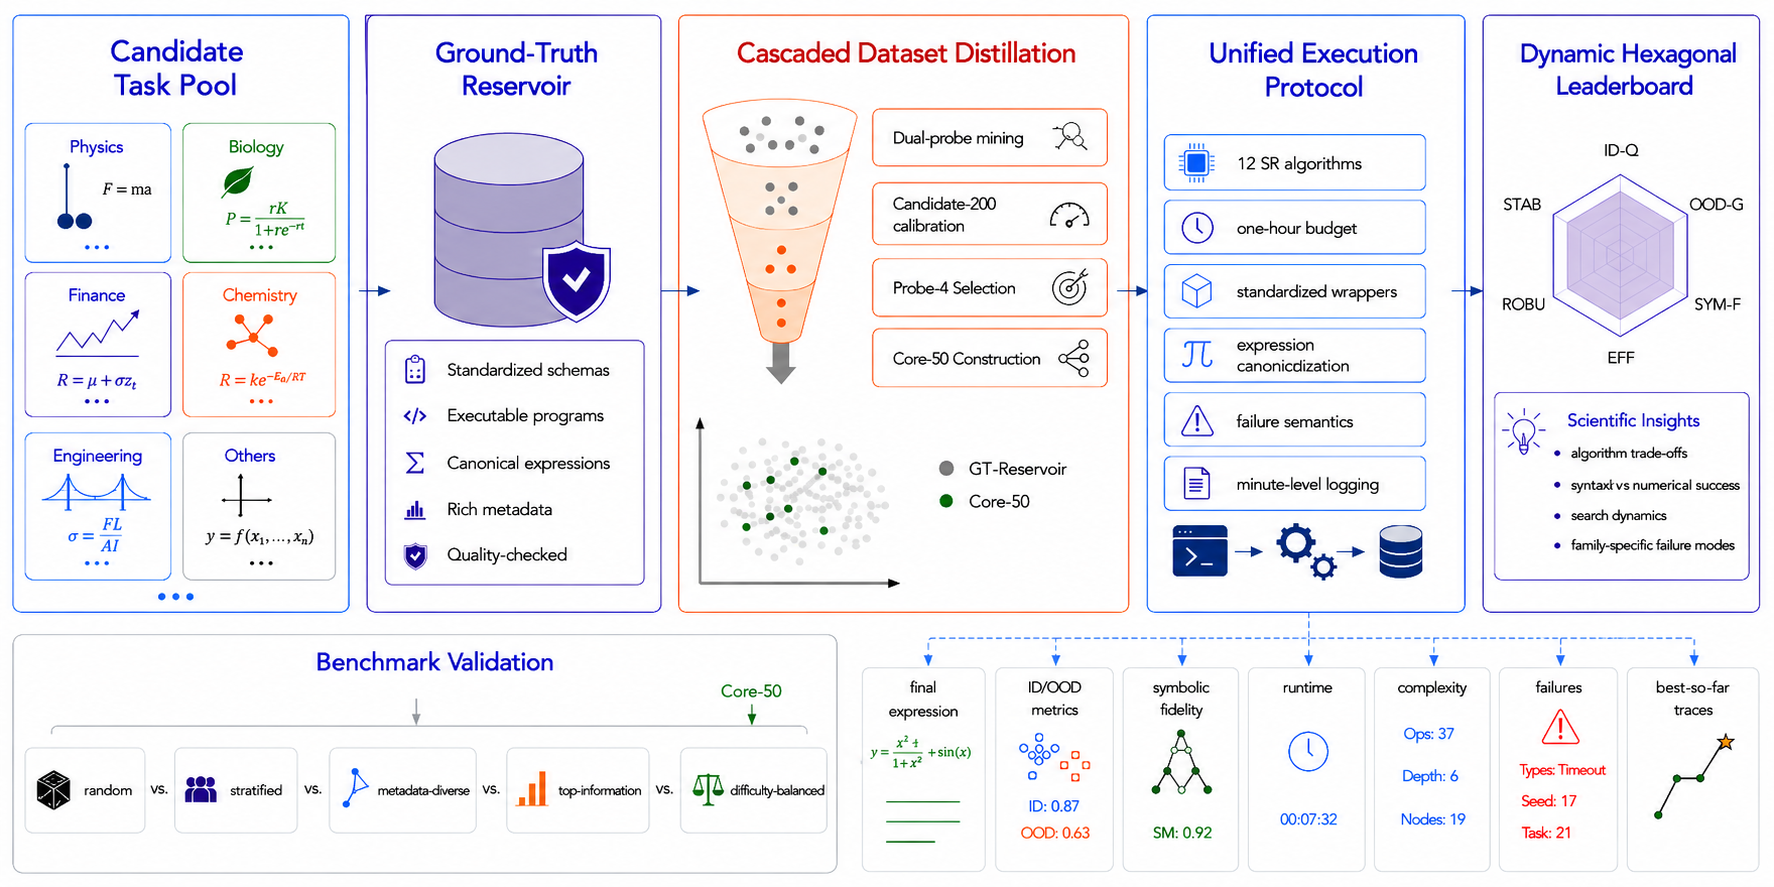
\includegraphics[width=\linewidth]{imgs/Article/figure01_pipeline}
\caption{\textbf{Overview of \arena{}}. A heterogeneous symbolic regression task pool is standardized into a quality-checked ground-truth reservoir, from which a compact and high-information Core-50 benchmark is distilled through cascaded dataset selection. The frozen Core-50 is evaluated under a unified execution protocol to produce a dynamic six-axis leaderboard and fine-grained search traces.}
\label{fig:symbolicarena-pipeline}
\end{figure}

\paragraph{Dataset reservoir.}
The dataset layer converts heterogeneous SR sources into a shared executable format. Each task is associated with standardized data splits, a ground-truth expression, structural metadata, and a canonical identity for semantic duplicate control. This standardized reservoir makes benchmark compression auditable: Core-50 is distilled from a consistently runnable and inspectable task pool rather than from loosely collected datasets.

\paragraph{Algorithm panel and execution protocol.}
The algorithm layer integrates 12 representative SR methods spanning evolutionary search, reinforcement learning, tree search, neural-guided search, transformer-based methods, and LLM-assisted approaches. Each method is accessed through a standardized wrapper that receives the same data contract, budget, seed, and output specification. A lightweight execution layer isolates method-specific environments while enforcing a common result schema, failure semantics, metric computation, expression canonicalization, and progress logging. Implementation details are provided in \cref{app:infra-cleaning}.

\paragraph{\core{} distillation engine.}
The distillation layer separates candidate discovery from final core selection. Candidate discovery uses PySR and LLM-SR as complementary single-seed probes to identify tasks that expose informative differences between classical and LLM-assisted SR methods. Core selection then uses four non-LLM probes, selected from the 12-algorithm calibration panel, to evaluate the full 664-task reservoir with three seeds. The final Core-50 is selected under constraints that balance structural coverage, response diversity, discriminability, redundancy control, difficulty, and stability.

\paragraph{Dynamic leaderboard engine.}
The leaderboard layer evaluates algorithms on the frozen \core{} under a fixed one-hour budget and five random seeds. In addition to final outputs, \arena{} stores best-so-far expressions at minute resolution, enabling analysis of anytime performance, symbolic recovery, complexity growth, robustness, and seed stability. The six leaderboard axes are normalized using fixed absolute definitions rather than relative ranks, so adding new algorithms does not change previously reported scores.

\paragraph{Design principle.}
\arena{} is designed to preserve informative differences among SR methods while keeping evaluation cost low enough for repeated use. The benchmark therefore does not simply select the easiest, hardest, or largest-gap tasks; instead, it distills a compact core that remains representative, discriminative, non-redundant, and stable under repeated evaluation.

% \section{Dataset Reservoir and Standardization}

% \subsection{Ground-truth filtering}

% \arena{} begins from a large candidate pool and filters tasks according to ground-truth availability and evaluation readiness. A task is retained if it has a valid ground-truth formula, train/ID/OOD splits, usable metadata, and a parsable expression representation. This yields
% \[
% D_{\mathrm{GT}} = 664.
% \]
% The resulting \reservoir{} is the population that \core{} is designed to represent.

% Reservoir composition is audited by source family, operator profile, formula complexity, and probe-derived difficulty bins. We keep the detailed composition plot in \cref{app:additional-figures} so the main text can focus on the distillation and validation evidence.

% \subsection{Metadata and expression standardization}

% Each dataset stores at least the following fields:
% \begin{verbatim}
% dataset_id, family, subgroup, basename, source_benchmark,
% ground_truth_formula, train_split, id_test_split, ood_test_split,
% n_features, sample_count, formula_complexity, operator_types,
% ood_type, dummy_variable_flag, semantic_duplicate_group
% \end{verbatim}

% All formulas are canonicalized into a unified expression representation, including canonical strings, prefix/postfix forms, expression trees, operator-normalized forms, constant-normalized forms, and Newick-like tree formats. This standardization enables symbolic equivalence testing, expression-tree comparison, operator and variable recovery, duplicate detection, and seed-level structural consistency.
\section{Dataset Reservoir and Standardization}
\label{sec:reservoir}

\arena{} begins from a large candidate pool of more than 800 symbolic regression tasks and filters them by ground-truth availability and evaluation readiness. A task is retained if it provides a valid ground-truth formula, fixed train/ID/OOD splits, usable metadata, and a parsable expression representation. This yields $|D_{\mathrm{GT}}| = 664.$

The resulting \reservoir{} is the parent population that \core{} is designed to represent. Its composition is audited by source family, operator profile, formula complexity, and difficulty bins; detailed statistics are provided in \cref{app:reservoir}.

Each retained dataset stores standardized provenance, split, formula, and structural metadata. All formulas are canonicalized into a unified expression representation, including canonical strings, prefix/postfix forms, expression trees, operator-normalized forms, constant-normalized forms, and Newick-like tree serializations. This standardization enables symbolic equivalence testing, expression-tree comparison, operator and variable recovery, duplicate detection, and seed-level structural consistency in later leaderboard evaluation. Detailed reservoir composition statistics are provided in \cref{fig:appendix-reservoir-composition}.

\begin{figure}[t]
\centering
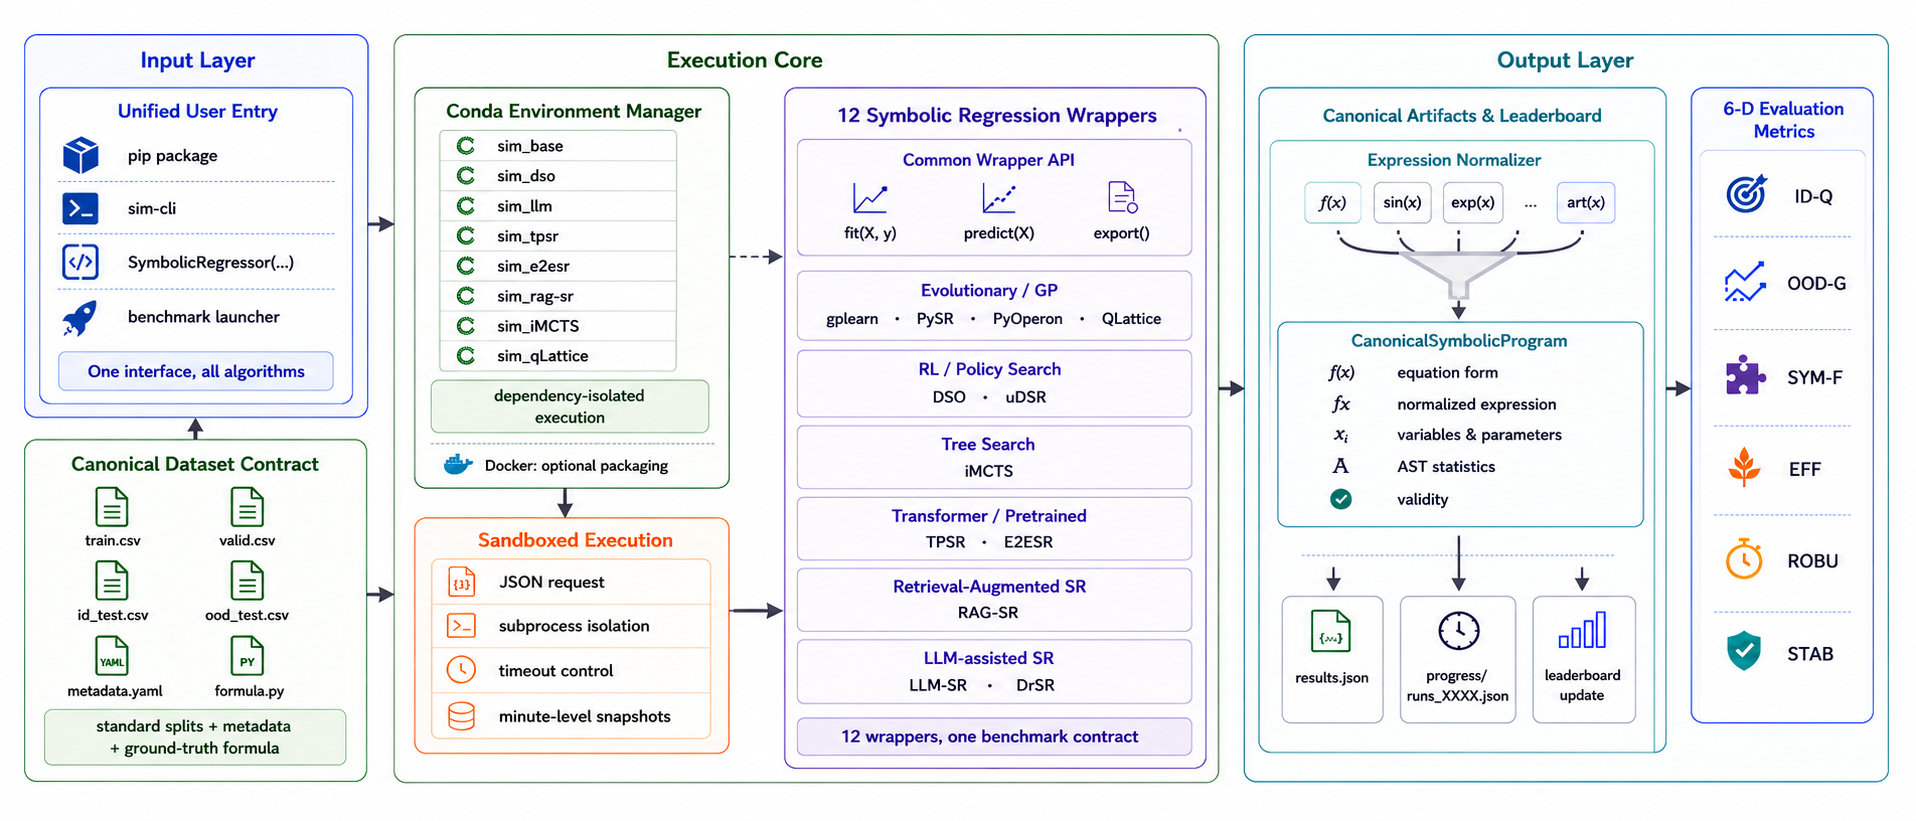
\includegraphics[width=0.95\linewidth]{imgs/Article/SAinfrastructure}
\caption{\textbf{\arena{} dataset reservoir and standardization pipeline.} Raw SR task sources are converted into a shared executable schema with validated splits, ground-truth formulas, metadata, canonical expression artifacts, and duplicate-control identities before entering benchmark distillation and leaderboard evaluation.}
\label{fig:sa-infrastructure}
\end{figure}

% \section{\core{} Distillation}

% The purpose of \core{} is not to create a small random subset of the reservoir. It is to create a compact benchmark that preserves the main structural coverage and algorithm-response conclusions of \reservoir{} while remaining cheap enough for repeated leaderboard evaluation. We therefore treat subset construction as a cascaded distillation problem: an 800+ raw candidate pool is filtered to the 664-task \reservoir{}, mined into the 200-task \candidate{} set with PySR/LLM-SR disagreement signals, calibrated with 12 methods, distilled to a four-method \probe{} panel, and finally compressed into the 50-task \core{} benchmark. Full formulas, quota derivations, and implementation details are given in \cref{app:core50-details}.

% \subsection{Candidate-200 mining}

% The first stage uses two complementary probes, PySR and LLM-SR, on all 664 ground-truth tasks:
% \[
% 664 \times 2 = 1328 \text{ runs}.
% \]
% PySR provides a strong non-LLM SR baseline, while LLM-SR provides a qualitatively different LLM-assisted search paradigm. Physical background descriptions are withheld in this stage, so the LLM probe is not selected merely because it can exploit semantic context.

% For each dataset, we compute ID and OOD disagreement between the two probes in clipped log-NMSE space. \candidate{} is not the top 200 by disagreement alone. It combines high-disagreement tasks, one-sided evaluability cases, and mid-gap tasks under source, subgroup, basename, and advantage-side caps. The resulting pool contains 140 high-discrimination tasks, 20 one-sided evaluability tasks, and 40 mid-gap tasks. Its role is calibration: it should expose method differences and failure modes, not serve as the final benchmark.

% \subsection{Probe-4 selection}

% We then run 12 integrated algorithms on \candidate{} with one seed:
% \[
% 200 \times 12 = 2400 \text{ runs}.
% \]
% The goal is to choose four non-LLM probes that are healthy enough to run at scale, complementary in behavior, and faithful to the broader 12-method panel's dataset-informativeness judgments. For a candidate four-method panel $P$, the selection score is
% \[
% \mathrm{Score}(P)=0.20H(P)+0.40F(P)+0.25C(P)+0.15V(P),
% \]
% where $H$ measures execution health, $F$ measures fidelity to the 12-method panel, $C$ measures behavioral complementarity, and $V$ measures dataset coverage. We additionally require taxonomy diversity and exclude methods whose role is already used in the dual-probe mining stage or whose behavior depends on LLM/RAG context.

% \begin{figure}[t]
% \centering
% \begin{minipage}{0.49\linewidth}
% \centering
% 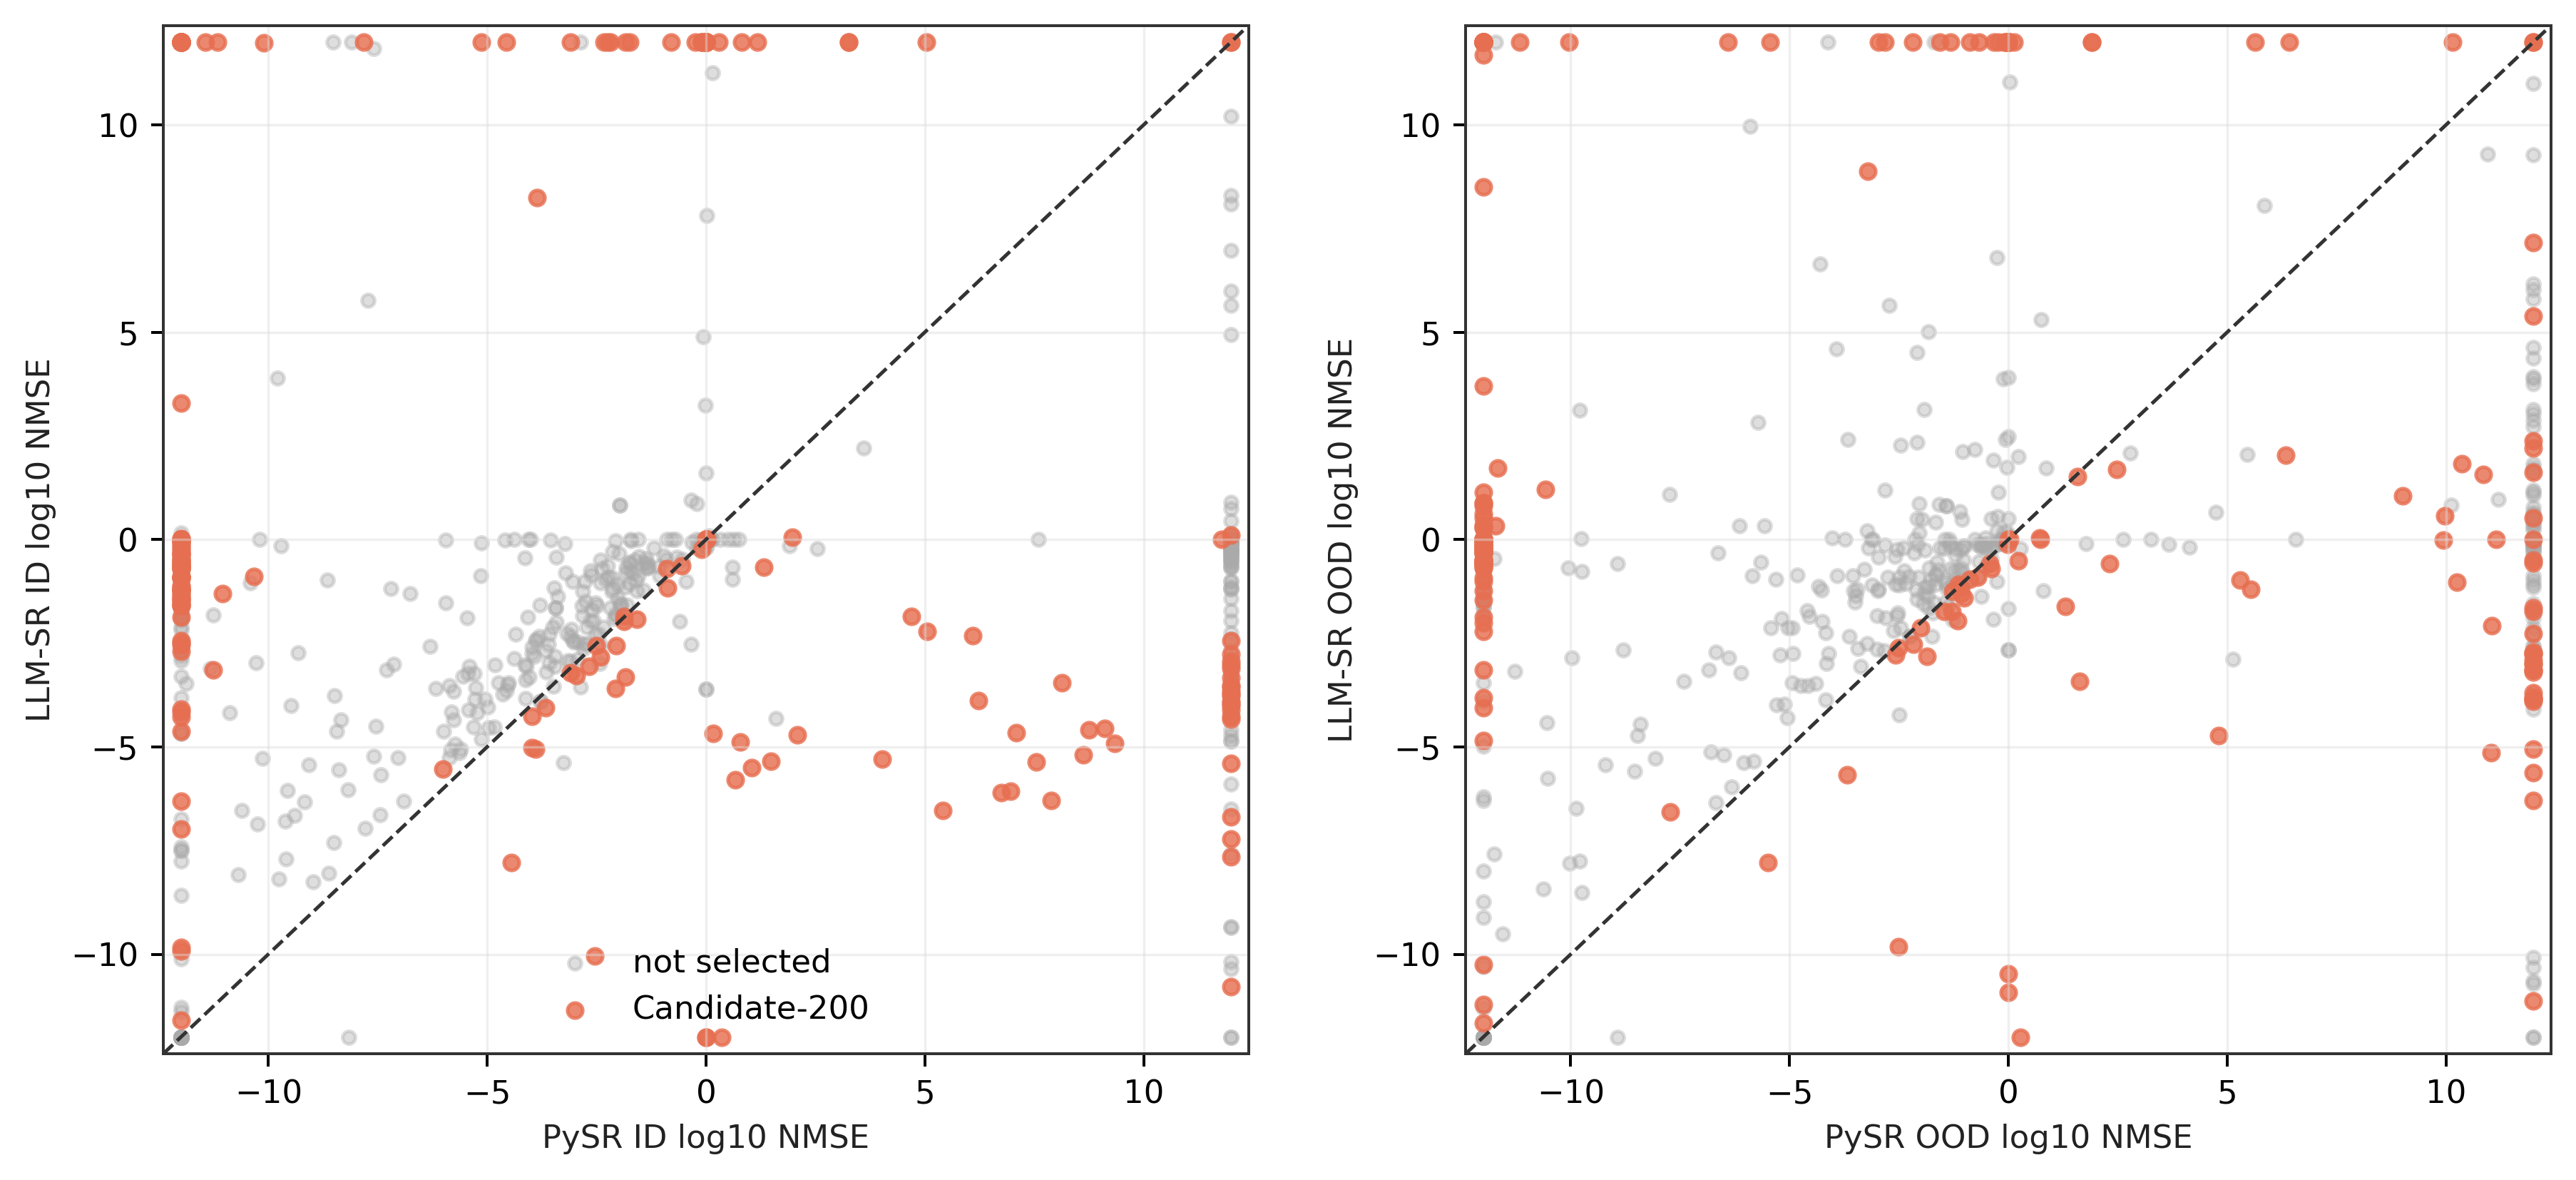
\includegraphics[width=\linewidth]{imgs/Appendix/figure03_dual_probe_scatter}
% \end{minipage}
% \hfill
% \begin{minipage}{0.49\linewidth}
% \centering
% 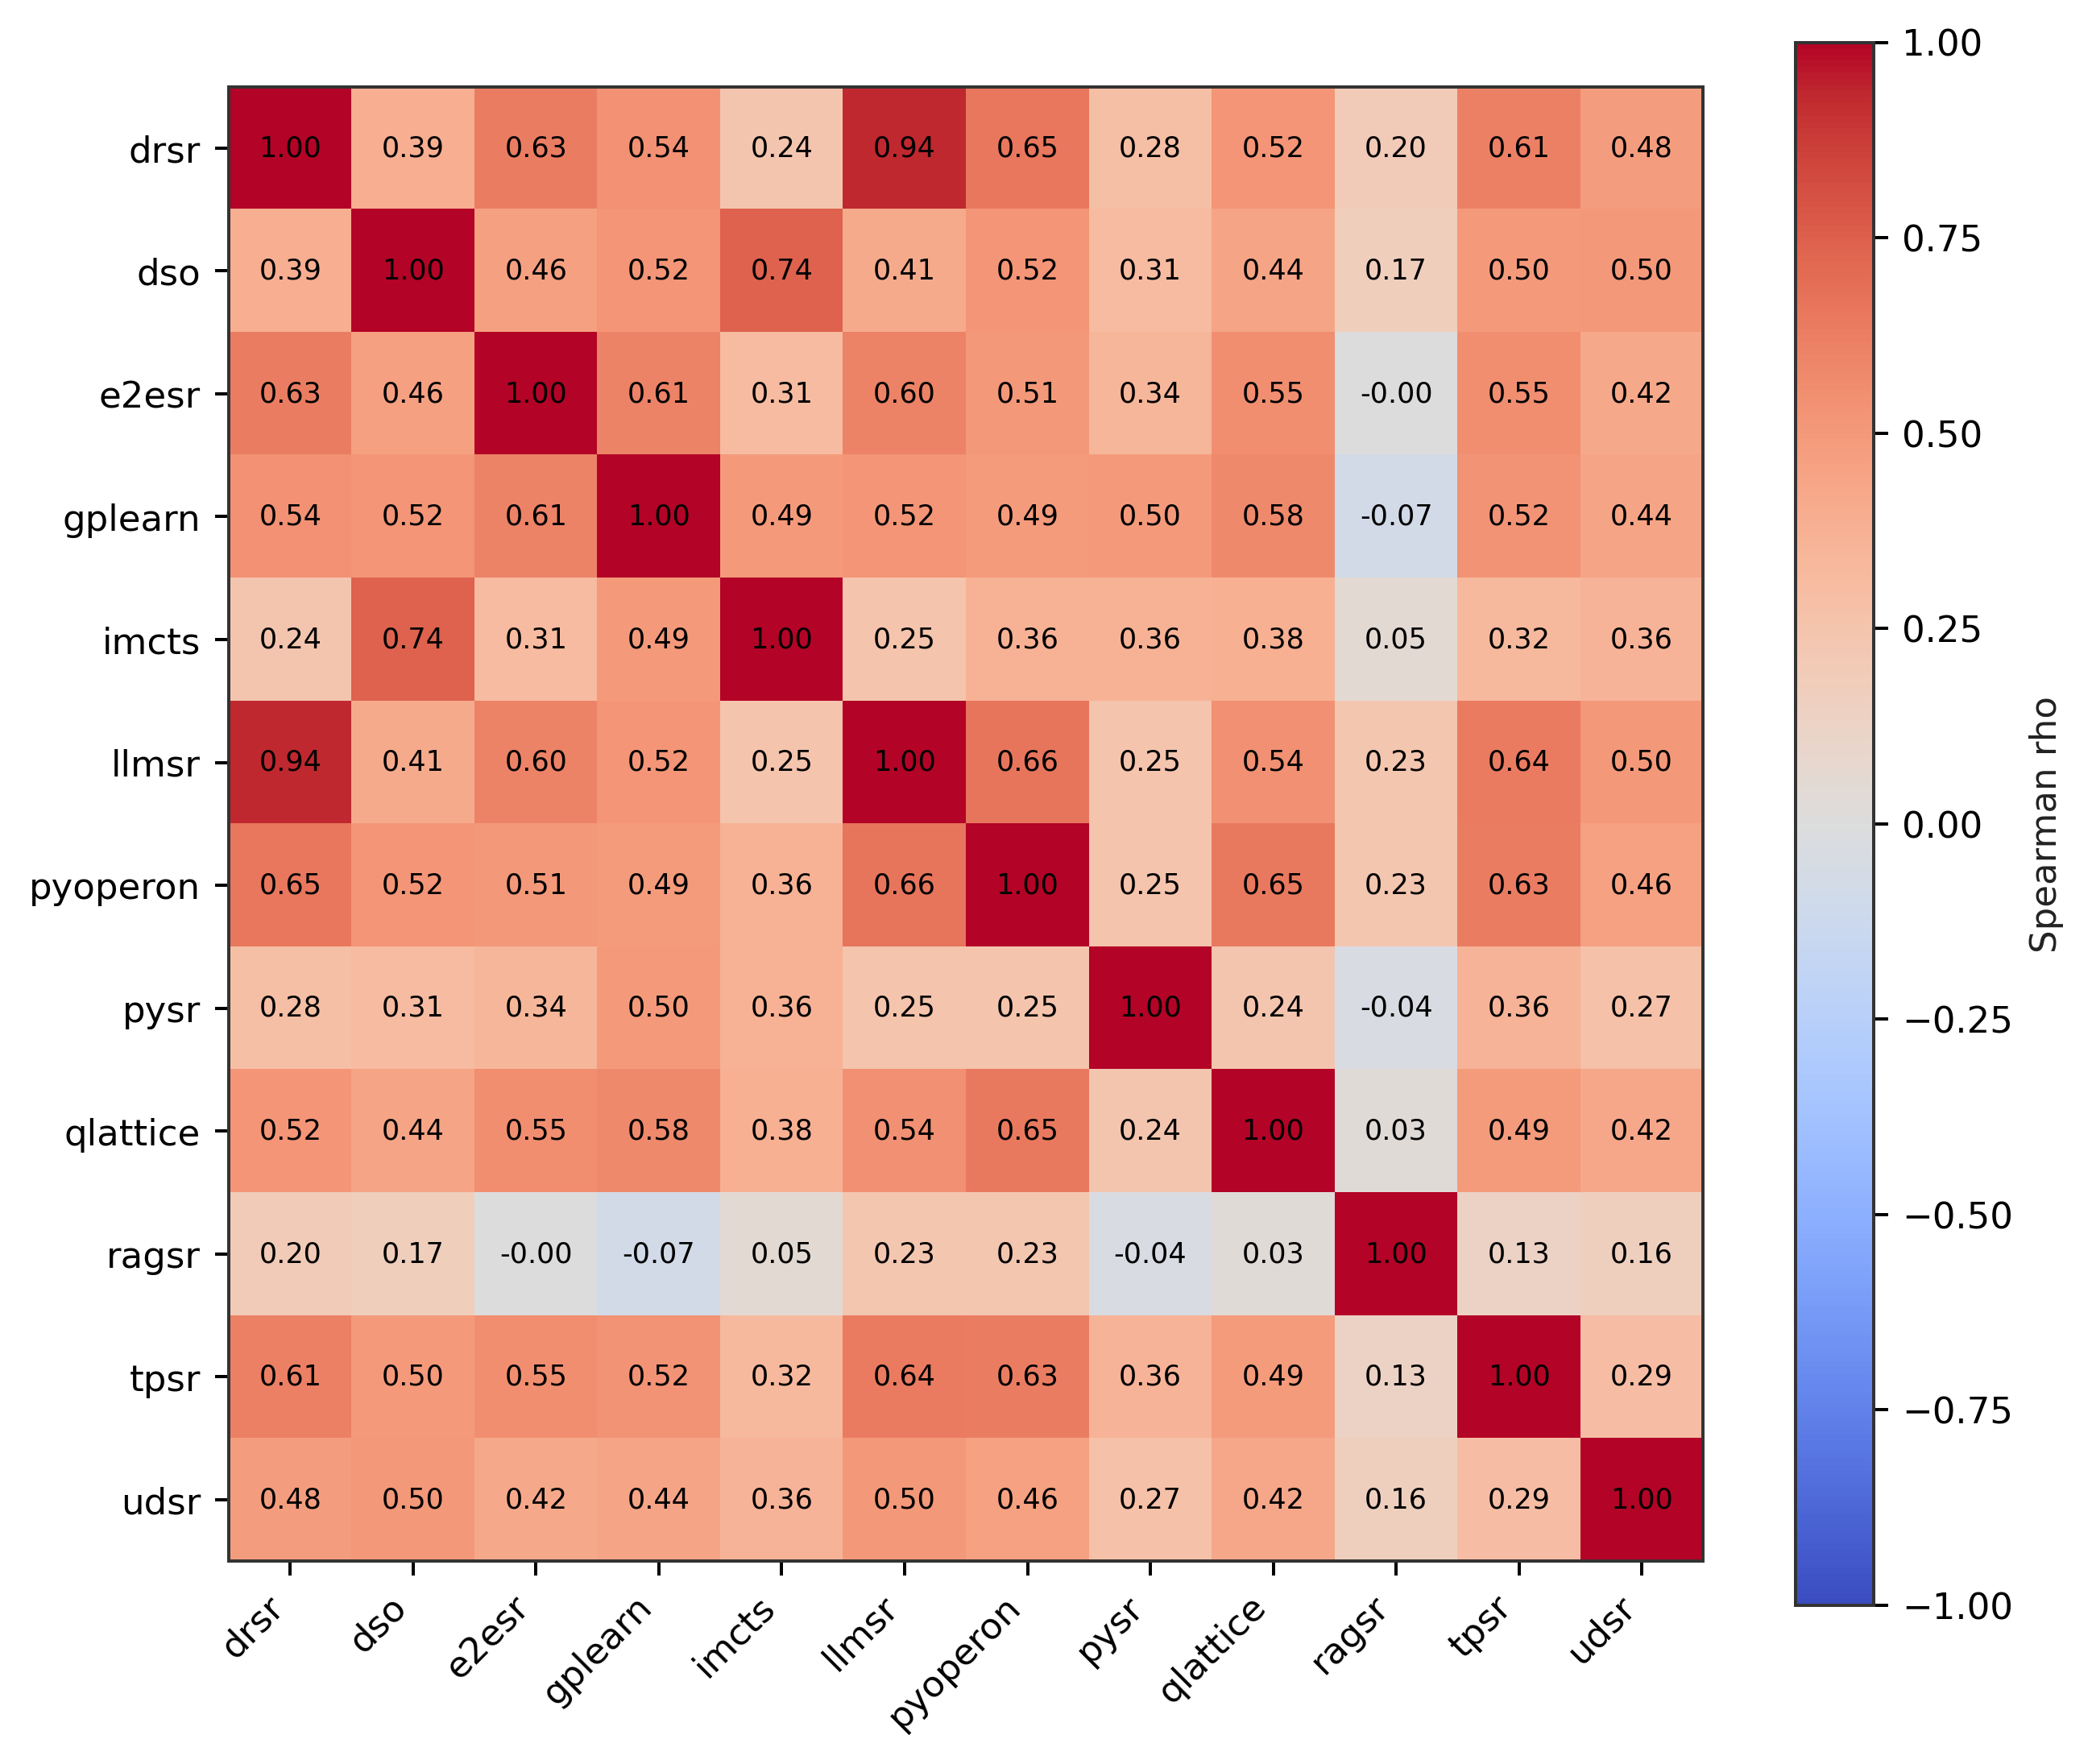
\includegraphics[width=\linewidth]{imgs/Article/figure07_algorithm_behavior_correlation}
% \end{minipage}
% \caption{Distillation diagnostics. Left: PySR/LLM-SR disagreement identifies high-information Candidate-200 regions without using physical background descriptions. Right: response correlation among the 12 calibrated algorithms prevents Probe-4 from collapsing into four redundant methods.}
% \label{fig:distillation-diagnostics}
% \end{figure}

% The final \probe{} is
% \[
% \{\mathrm{DSO}, \mathrm{PyOperon}, \mathrm{iMCTS}, \mathrm{uDSR}\}.
% \]
% This panel is not chosen because it has the highest NMSE-only score. It is chosen because it satisfies the health and taxonomy constraints while remaining a compact surrogate for broader algorithm-panel behavior. \Cref{app:core50-details} reports the top NMSE-only combinations and the final selected panel for auditability.

% \subsection{Probe4-Full response profiles}

% We run \probe{} on all 664 reservoir tasks with three seeds:
% \[
% 664 \times 4 \times 3 = 7968 \text{ runs}.
% \]
% Each run records status, validity, train/validation/ID/OOD metrics, runtime, expression, complexity, and failure reason. NMSE values are converted to clipped log space:
% \[
% \ell(\mathrm{NMSE})=\mathrm{clip}(\log_{10}(\max(\mathrm{NMSE},10^{-12})),-12,12).
% \]
% For each dataset--probe pair, seed-level results are aggregated into median ID/OOD log-NMSE, seed IQR, valid rate, runtime, and complexity. These response profiles are the only result-derived inputs used to score dataset informativeness.

% \subsection{\core{} objective and constraints}

% Each dataset has a structural profile and a Probe-4 response profile. The structural profile contains static metadata such as family, subgroup, semantic duplicate group, feature count, sample scale, formula complexity, operator type, OOD type, and dummy-variable status. The response profile contains Probe-4 median ID/OOD performance, ID-to-OOD degradation, valid-output pattern, winner probe, and seed-level stability.

% The main selection objective is:
% \[
% S^*=\arg\max_{S\subset D,\ |S|=50}
% \left[
% 0.45\,\mathrm{Coverage}(S)
% +0.35\,\mathrm{MeanInfo}(S)
% +0.20\,\mathrm{Balance}(S)
% \right].
% \]
% Here, $\mathrm{Coverage}$ preserves both structural and response-space coverage, $\mathrm{MeanInfo}$ rewards tasks that discriminate between probes while remaining seed-stable, and $\mathrm{Balance}$ penalizes distributional drift from the 664-task reservoir. Dataset information is summarized as
% \[
% \mathrm{Info}_i=\mathrm{Discrimination}_i \times \mathrm{Stability}_i.
% \]
% Intuitively, a high-information dataset is one where the probes behave differently for stable reasons, rather than because of random seeds, invalid outputs, or timeout artifacts.

% Hard constraints prevent the objective from collapsing into a pathological subset. They cap semantic duplicates, basename/source concentration, subgroup concentration, invalid-prone and one-sided cases, and extreme-difficulty cases, while preserving family and difficulty coverage. No source family receives a hand-written special rule: family quotas are derived from reservoir proportions with uniform smoothing. The released manifest also excludes result-derived columns such as probe gap, priority score, and selected advantage side; final benchmark materialization is audited using dataset identity and static metadata only. The detailed coverage map is provided in \cref{app:additional-figures}.

% \subsection{\core{} validation}

% After selection, we validate \core{} against the full reservoir using Probe4-Full results. The validation checks whether the 50-task subset preserves method ranking, pairwise preferences, aggregate scores, and distributional structure from the 664-task reservoir. It also compares \core{} against repeated random and family-stratified subsets, together with curated alternatives such as top-information, metadata-diverse, and difficulty-balanced subsets. The central validation claim is not that 50 tasks replace the full reservoir, but that \core{} is a high-information development benchmark whose conclusions remain aligned with the larger pool.

% \begin{table}[t]
% \centering
% \small
% \caption{\core{} validation against alternative 50-task selectors. Higher is better for all columns. The table complements the aggregate-error and rank-correlation checks in the experiments section.}
% \label{tab:core50-baseline-main}
% \resizebox{\linewidth}{!}{%
% \begin{tabular}{lrrrrrr}
% \toprule
% Subset & Coverage & Mean info & Rank fidelity & Stability & Non-red. & Diff. balance \\
% \midrule
% \core{} & 0.838 & 0.471 & 1.000 & 0.835 & 0.769 & 0.892 \\
% top-info-50 & 0.784 & 0.691 & 1.000 & 0.911 & 0.860 & 0.780 \\
% metadata-diverse-50 & 0.635 & 0.085 & 1.000 & 0.735 & 0.860 & 0.601 \\
% difficulty-balanced-50 & 0.817 & 0.637 & 1.000 & 0.883 & 0.920 & 0.999 \\
% random-50 avg & 0.835 & 0.187 & 0.983 & 0.705 & 0.970 & 0.908 \\
% family-stratified random-50 avg & 0.815 & 0.191 & 0.995 & 0.696 & 0.968 & 0.909 \\
% \bottomrule
% \end{tabular}
% }
% \end{table}

\section{\core{} Distillation}
\label{sec:core50-distillation}

\paragraph{Goal.}
The purpose of \core{} is not to create a small random subset of the reservoir, but to construct a compact benchmark that preserves the main structural coverage and algorithm-response conclusions of \reservoir{} while remaining cheap enough for repeated leaderboard evaluation. We therefore formulate subset construction as a cascaded distillation problem: an 800+ raw task pool is filtered into the 664-task \reservoir{}, mined into a 200-task calibration set, used to select a compact non-LLM probe panel, and finally distilled into the 50-task \core{} benchmark. Full formulas, quota derivations, implementation details, and audit tables are provided in \cref{app:core50-details}.

\paragraph{Candidate-200 mining.}
The first stage uses two complementary probes, PySR and LLM-SR, on all 664 ground-truth tasks, resulting in $664 \times 2 = 1328$ single-seed runs. Physical background descriptions are withheld, so the LLM-based probe cannot directly exploit semantic context. For each dataset, ID and OOD disagreement between the two probes is computed in clipped log-NMSE space. The 200-task \candidate{} set is not obtained by simply taking the top-200 disagreement cases. Instead, it combines high-disagreement tasks, one-sided evaluability cases, and mid-gap tasks under source, subgroup, basename, and advantage-side caps. The resulting pool contains 140 high-discrimination tasks, 20 one-sided evaluability tasks, and 40 mid-gap tasks. Its role is calibration: it exposes method differences and failure modes, but is not used as the final benchmark.

\paragraph{Probe-4 selection.}
We next run the 12 integrated algorithms on \candidate{} with one seed, producing $200 \times 12 = 2400$ calibration runs. The goal is not to choose the four strongest algorithms, but to choose a small non-LLM probe panel that is healthy enough to run at scale, behaviorally complementary, and faithful to the dataset-informativeness judgments of the broader 12-method panel. For a candidate four-method panel \(P\), the selection score is
\[
\mathrm{Score}(P)
=
0.20H(P)
+
0.40F(P)
+
0.25C(P)
+
0.15V(P),
\]
where \(H\) measures execution health, \(F\) measures fidelity to the 12-method panel, \(C\) measures behavioral complementarity, and \(V\) measures dataset coverage. Taxonomy constraints require at least three algorithmic paradigms, and construction-role constraints exclude methods whose behavior depends on LLM/RAG context or whose role is already used in dual-probe mining. The final \probe{} is selected as $\{\mathrm{DSO}, \mathrm{PyOperon}, \mathrm{iMCTS}, \mathrm{uDSR}\}$, yielding a compact surrogate that spans policy search, evolutionary GP, tree search, and neural-guided SR.

% \paragraph{Core-50 construction.}
% The selected \probe{} is evaluated on all 664 reservoir tasks with three seeds: $664 \times 4 \times 3 = 7968$ runs. These Probe4-Full runs define a response profile for each dataset, including median ID/OOD performance, ID-to-OOD degradation, valid-output patterns, and seed stability. Together with static structural metadata, these profiles are used to select \core{}:
% \[
% S^*
% =
% \arg\max_{S\subset D,\ |S|=50}
% \left[
% 0.45\,\mathrm{Coverage}(S)
% +
% 0.35\,\mathrm{MeanInfo}(S)
% +
% 0.20\,\mathrm{Balance}(S)
% \right].
% \]
% Here, \(\mathrm{Coverage}\) preserves both structural and response-space diversity, \(\mathrm{MeanInfo}\) rewards tasks that separate probes for stable reasons, and \(\mathrm{Balance}\) controls difficulty and failure-mode drift from the 664-task reservoir. Hard constraints cap semantic duplicates, basename concentration, subgroup concentration, invalid-prone tasks, one-sided cases, and extreme-difficulty cases. Family quotas are derived from reservoir proportions with uniform smoothing, so no source family receives a hand-written special rule. The constrained objective is optimized by greedy initialization, local swaps, and random restarts.

% Once validated, \core{} is frozen as the official development benchmark. The Probe4-Full results are used only for benchmark construction and are not reused as final leaderboard results. The formal leaderboard is recomputed independently by running all 12 algorithms on the frozen \core{} with five seeds: $12 \times 50 \times 5 = 3000$ formal evaluation runs.
\paragraph{Core-50 construction.}
The selected \probe{} is evaluated on all 664 reservoir tasks with three seeds, resulting in \(664 \times 4 \times 3 = 7968\) Probe4-Full runs. These runs, together with static dataset metadata, are used to select a 50-task subset by optimizing
\[
S^*
=
\arg\max_{S\subset D,\ |S|=50}
\left[
0.45\,\mathrm{Coverage}(S)
+
0.35\,\mathrm{MeanInfo}(S)
+
0.20\,\mathrm{Balance}(S)
\right].
\]
Here, \(\mathrm{Coverage}\) preserves structural and response-space diversity, \(\mathrm{MeanInfo}\) rewards stable probe-discriminative tasks, and \(\mathrm{Balance}\) controls difficulty and failure-mode drift. The optimization is performed under hard constraints on duplicates, family/subgroup concentration, invalid-prone cases, one-sided cases, and extreme-difficulty tasks; full definitions are given in \cref{app:core50-details}.

\paragraph{Validation.}
The selected \core{} is validated against the full 664-task reservoir and five subset-selection baselines: random-50, family-stratified random-50, metadata-diverse-50, top-information-50, and difficulty-balanced-50. The validation checks whether \core{} preserves reservoir-level method ordering, pairwise preferences, aggregate scores, structural distribution, difficulty balance, and failure-mode coverage. After validation, \core{} is frozen, and the final leaderboard is recomputed independently using all 12 algorithms with five seeds, yielding \(12 \times 50 \times 5 = 3000\) formal evaluation runs.

\section{Dynamic Leaderboard}

After \core{} is frozen, \arena{} constructs the formal leaderboard by running 12 algorithms on 50 datasets with five seeds:
\[
12 \times 50 \times 5 = 3000 \text{ clean runs}.
\]
Each run uses a one-hour time limit and saves the best-so-far expression every minute. This yields
\[
3000 \times 60 = 180000
\]
best-so-far expression snapshots.

\subsection{Unified execution}
All algorithms share the same dataset loader, split definitions, time limit, random seed interface, metric computation, expression parsing, canonicalization, result logging, and failure handling. This reduces engineering-related unfairness between methods.

\subsection{Snapshot logging}
Each final run stores algorithm, dataset, seed, status, validity, ID/OOD NMSE, raw expression, canonical expression, expression tree, complexity, and runtime. Each minute-level snapshot stores minute index, best expression, canonical expression, expression tree, ID/OOD NMSE, and complexity.

\subsection{Search-dynamics analysis}
Because \arena{} logs the search trajectory, it supports analysis of final performance, anytime performance, time-to-threshold, time-to-discovery, complexity-over-time, symbolic similarity-over-time, stagnation, and failure modes. This makes the leaderboard dynamic and diagnostic rather than merely rank-based.

\section{Hexagonal Evaluation Protocol}

\arena{} defines a fixed, absolute, 0--100 hexagonal metric protocol. Scores do not depend on the current set of algorithms and therefore do not drift when the leaderboard grows. Five axes are computed from the clean \core{} leaderboard: ID-Q, OOD-G, SYM-F, EFF, and STAB. The sixth axis, ROBU, is a standardized noisy-training extension track. When all algorithms have completed the noisy track, the full six-axis profile is reported; otherwise, the clean-track profile is reported with ROBU marked as pending rather than imputed.
The main text reports the resulting clean-track heatmap in \cref{fig:hexagon-heatmap}; per-algorithm small multiples and axis-correlation diagnostics are provided in \cref{app:additional-figures}.

All NMSE-based metrics use
\[
\phi(e)=1-\frac{\mathrm{clip}(\log_{10}(\max(e,10^{-12})),-12,2)+12}{14},
\]
so that $\phi(e)\in[0,1]$. Invalid, timeout, unparsable, NaN/Inf, wrong-signature, or unevaluable outputs are assigned $e=10^2$ and therefore $\phi(e)=0$.

\subsection{ID-Q: In-distribution quality}
\[
\mathrm{ID\text{-}Q}(a)=100\cdot\frac{1}{50}\sum_{d\in D}\phi\left(\mathrm{median}_s e^{id}_{a,d,s}\right).
\]

\subsection{OOD-G: Out-of-distribution generalization}
Let
\[
q^{ood}_{a,d}=\phi(\mathrm{median}_s e^{ood}_{a,d,s}).
\]
Define the ID-to-OOD retention as
\[
r^{ood}_{a,d}=1-\mathrm{clip}\left(\frac{\left[\log_{10}\frac{\tilde e^{ood}_{a,d}+\epsilon}{\tilde e^{id}_{a,d}+\epsilon}\right]_+}{4},0,1\right).
\]
Then
\[
\mathrm{OOD\text{-}G}(a)=100\cdot\frac{1}{50}\sum_{d\in D}(0.7q^{ood}_{a,d}+0.3r^{ood}_{a,d}).
\]

\subsection{SYM-F: Symbolic fidelity}
For each expression, compute CAS equivalence, dense-probe numeric equivalence, tree similarity, variable F1, and operator F1. The single-seed score is
\[
m^{sym}_{a,d,s}=\begin{cases}
1, & Eq_{a,d,s}=1,\\
0.3T_{a,d,s}+0.2SOF1_{a,d,s}, & Eq_{a,d,s}=0.
\end{cases}
\]
Then
\[
\mathrm{SYM\text{-}F}(a)=100\cdot\frac{1}{50}\sum_{d\in D}\frac{1}{5}\sum_{s=1}^{5}m^{sym}_{a,d,s}.
\]

\subsection{EFF: Efficiency}
Minute-level quality is
\[
q^{time}_{a,d,s}(t)=0.5\phi(e^{id,best}_{a,d,s}(t))+0.5\phi(e^{ood,best}_{a,d,s}(t)).
\]
The run-level AUC is
\[
AUC_{a,d,s}=\frac{1}{60}\sum_{t=1}^{60}q^{time}_{a,d,s}(t).
\]
Then
\[
\mathrm{EFF}(a)=100\cdot\frac{1}{50}\sum_{d\in D}\mathrm{median}_s AUC_{a,d,s}.
\]

\subsection{ROBU: Noise robustness}
ROBU uses noisy-training experiments with $\Sigma=\{0.01,0.05,0.10\}$. Training labels are perturbed by
\[
y'=y+\sigma\cdot\mathrm{std}(y)\cdot\epsilon,\quad \epsilon\sim\mathcal N(0,1),
\]
while ID/OOD tests remain clean. The noisy quality is
\[
q^{noise}_{a,d,\sigma}=0.5\phi(\tilde e^{id,noise}_{a,d,\sigma})+0.5\phi(\tilde e^{ood,noise}_{a,d,\sigma}).
\]
The retention score is
\[
ret_{a,d,\sigma}=\mathrm{clip}\left(\frac{q^{noise}_{a,d,\sigma}}{\max(q^{clean}_{a,d},0.25)},0,1\right).
\]
Then
\[
\mathrm{ROBU}(a)=100\cdot\frac{1}{50|\Sigma|}\sum_{d\in D}\sum_{\sigma\in\Sigma}(0.7q^{noise}_{a,d,\sigma}+0.3ret_{a,d,\sigma}).
\]
The noisy track adds $12\times 50\times 5\times 3=9000$ runs. Since ROBU requires additional experiments, it is never backfilled from clean-track runs.

\subsection{STAB: Effective stability}
STAB measures whether an algorithm stably produces valid and useful formulas, not merely whether it stably fails. Pure stability is
\[
PureStab_{a,d}=0.4N_{a,d}+0.3V_{a,d}+0.3C_{a,d},
\]
where $N$ is numerical IQR stability, $V$ is valid seed rate, and $C$ is structural consistency across seed pairs. A performance correction is
\[
q^{perf}_{a,d}=0.4q^{id}_{a,d}+0.3q^{oodG}_{a,d}+0.3q^{sym}_{a,d}.
\]
The final stability score is
\[
\mathrm{STAB}(a)=100\cdot\frac{1}{50}\sum_{d\in D} PureStab_{a,d}\sqrt{q^{perf}_{a,d}}.
\]

\subsection{Optional HexaScore}
We report the available axes separately and do not impute missing \rob{} values. For auxiliary ranking, a six-axis HexaScore is computed only after the noisy-training track has been completed:
\[
\mathrm{HexaScore}(a)=100\cdot\left(\prod_{k=1}^{6}\max\left(\frac{M_k(a)}{100},10^{-6}\right)\right)^{1/6}.
\]

\section{Experiments}

We evaluate \arena{} along three questions: whether \core{} preserves the probe-level conclusions of the 664-task reservoir, whether the 12-algorithm execution layer is healthy enough for leaderboard use, and whether the resulting leaderboard exposes meaningful algorithmic differences.

\subsection{Experimental setup}

The complete clean evaluation pipeline contains four stages. First, PySR and LLM-SR are run once on the 664-task reservoir, producing $664\times2=1328$ dual-probe runs. Second, 12 algorithms are run once on \candidate{}, producing $200\times12=2400$ calibration runs. Third, the selected \probe{} panel is run on the full reservoir with three seeds, producing $664\times4\times3=7968$ runs. Fourth, all 12 algorithms are run on \core{} with five seeds under a one-hour budget, producing $12\times50\times5=3000$ leaderboard runs.

The 12-method panel is designed to cover the main algorithmic paradigms used in modern SR rather than a single family of GP solvers. It includes classical and modern evolutionary methods (gplearn, PyOperon, PySR, QLattice, RAG-SR), reinforcement-learning and neural-guided methods (DSO, uDSR), tree-search and transformer/planning methods (iMCTS, E2ESR, TPSR), and LLM-assisted equation-discovery systems (LLM-SR, DRSR). \Cref{app:evaluated-baselines} gives the detailed baseline descriptions, including each method's search paradigm, integration contract, and interpretation caveats.

All reported NMSE values use clipped log space:
\[
\log_\mathrm{NMSE}=\mathrm{clip}(\log_{10}(\max(\mathrm{NMSE},10^{-12})),-12,12).
\]
For aggregate leaderboard tables, missing or unevaluable metrics are assigned the worst clipped value before averaging. This prevents invalid outputs from being silently removed.

\subsection{Probe4-Full health and readiness}

The \probe{} full-reservoir stage completed all expected $7968$ runs. Among them, $7616$ runs produced valid outputs. Completion was balanced across the three seeds, each with $2656$ finished runs. Method-level valid rates were $96.9\%$ for DSO, $98.5\%$ for iMCTS, $87.7\%$ for PyOperon, and $99.2\%$ for uDSR. The health gate used for selecting \probe{} is applied during the \candidate{} calibration stage; PyOperon's broader-reservoir valid rate drops below $90\%$, but it remains useful as an evolutionary-GP probe because invalid-prone datasets are explicitly handled by eligibility and limited-quota filters. The postprocessed dataset-level table marks all 664 datasets as complete, with 540 eligible datasets and 124 limited-quota datasets. This makes the Probe4-Full result suitable for \core{} selection.

\subsection{\core{} representativeness}

We compare \core{} against the full 664-task reservoir using the four Probe-4 methods. On the full reservoir, the OOD ranking is
\[
\mathrm{uDSR} \prec \mathrm{iMCTS} \prec \mathrm{DSO} \prec \mathrm{PyOperon},
\]
where lower median log OOD NMSE is better. The same ordering is obtained on \core{}: the paired full-reservoir/\core{} OOD scores are $-5.216/-5.431$ for uDSR, $-4.292/-4.248$ for iMCTS, $-2.305/-2.423$ for DSO, and $-0.410/-0.431$ for PyOperon. The Spearman and Kendall rank correlations between full-reservoir and \core{} Probe-4 aggregate OOD scores are both $1.0$, and all six pairwise method preferences agree.

We also compare \core{} with random and family-stratified random 50-task subsets, plus deterministic alternatives that select by information, metadata diversity, response-space K-medoids, or difficulty balance. \core{} has an aggregate-score MAE of $0.1388$ against the full-reservoir Probe-4 scores, compared with $0.4949$ for random-50 average, $0.5243$ for family-stratified random-50 average, $0.5060$ for metadata-diverse selection, $0.6044$ for response-space K-medoids, $1.0339$ for top-information, and $1.0430$ for difficulty-balanced selection. Thus \core{} reduces aggregate-score error by $72.0$--$86.7\%$ relative to these baselines. Top-information selection has a marginally higher objective score and the highest mean information, but its full-reservoir fidelity is substantially worse. \Cref{tab:core50-ablation-summary} summarizes the curated selector comparison; full definitions are in \cref{app:core50-details}.

\subsection{Leaderboard execution health}

The \core{} leaderboard stage produced all expected 3000 final result files, with no missing or ambiguous artifacts. The status distribution was 2982 \texttt{ok}, 9 \texttt{timed\_out}, and 9 \texttt{no\_valid\_output}. Every algorithm has exactly 250 runs. Ten of the twelve algorithms have 100\% valid-output rate; PyOperon and QLattice have 98.4\% and 98.0\%, respectively.

\begin{table}[t]
\centering
\small
\caption{\textbf{Clean \core{} leaderboard.} Methods are evaluated over 50 datasets and five seeds, ranked by penalized OOD log NMSE (lower is better), and reported with ID log NMSE plus symbolic-fidelity diagnostics. Exact is an SA-style exact-equivalence rate; TreeSim is the TED/NED-style tree-similarity component used by \symf{} (higher is better).}
\label{tab:clean-leaderboard-summary}
\resizebox{\linewidth}{!}{%
\begin{tabular}{rlrrrrrrr}
\toprule
\textbf{Rank} & \textbf{Algorithm} & \textbf{Valid} & \textbf{Metric} & \textbf{ID log} & \textbf{OOD log} & \textbf{\symf{}} & \textbf{Exact \%} & \textbf{TreeSim} \\
\midrule
1 & uDSR & 1.000 & 1.000 & $-6.920$ & $-5.646$ & 36.8 & 24.0 & 0.129 \\
2 & iMCTS & 1.000 & 0.968 & $-4.842$ & $-3.960$ & 41.5 & 30.8 & 0.185 \\
3 & PySR & 1.000 & 0.960 & $-3.848$ & $-3.055$ & 43.6 & 34.0 & 0.242 \\
4 & DSO & 1.000 & 0.972 & $-2.984$ & $-2.458$ & 31.3 & 18.0 & 0.183 \\
5 & DRSR & 1.000 & 1.000 & $-3.396$ & $-2.087$ & 26.8 & 12.0 & 0.098 \\
6 & LLM-SR & 1.000 & 0.992 & $-2.958$ & $-1.420$ & 27.3 & 12.8 & 0.102 \\
7 & gplearn & 1.000 & 1.000 & $-2.013$ & $-1.207$ & 20.0 & 8.0 & 0.085 \\
8 & QLattice & 0.980 & 0.972 & $-2.273$ & $-0.780$ & 17.8 & 4.8 & 0.029 \\
9 & TPSR & 1.000 & 0.996 & $0.200$ & $0.896$ & 15.2 & 0.4 & 0.035 \\
10 & PyOperon & 0.984 & 0.840 & $-0.070$ & $1.079$ & 11.3 & 0.0 & 0.026 \\
11 & E2ESR & 1.000 & 0.800 & $2.049$ & $2.891$ & 12.4 & 0.0 & 0.001 \\
12 & RAG-SR & 1.000 & 0.964 & $3.253$ & $3.788$ & 15.7 & 1.6 & 0.000 \\
\bottomrule
\end{tabular}
}
\end{table}

The expanded metric set follows prior SR benchmark practice: SRBench reports numerical quality together with symbolic-solution and cost indicators; SRSD adds normalized tree-edit distance for expression structure; LLM-SRBench reports ID/OOD NMSE and symbolic accuracy. Accordingly, \cref{tab:clean-leaderboard-summary} keeps the OOD ranking as the primary leaderboard key while exposing whether a method's numerical score is accompanied by symbolic recovery. These results are not intended as the final scientific conclusion of SR as a field. Instead, they demonstrate that SymbolicArena produces a complete, comparable, multi-algorithm evaluation substrate with explicit failure accounting.

\begin{figure}[t]
\centering
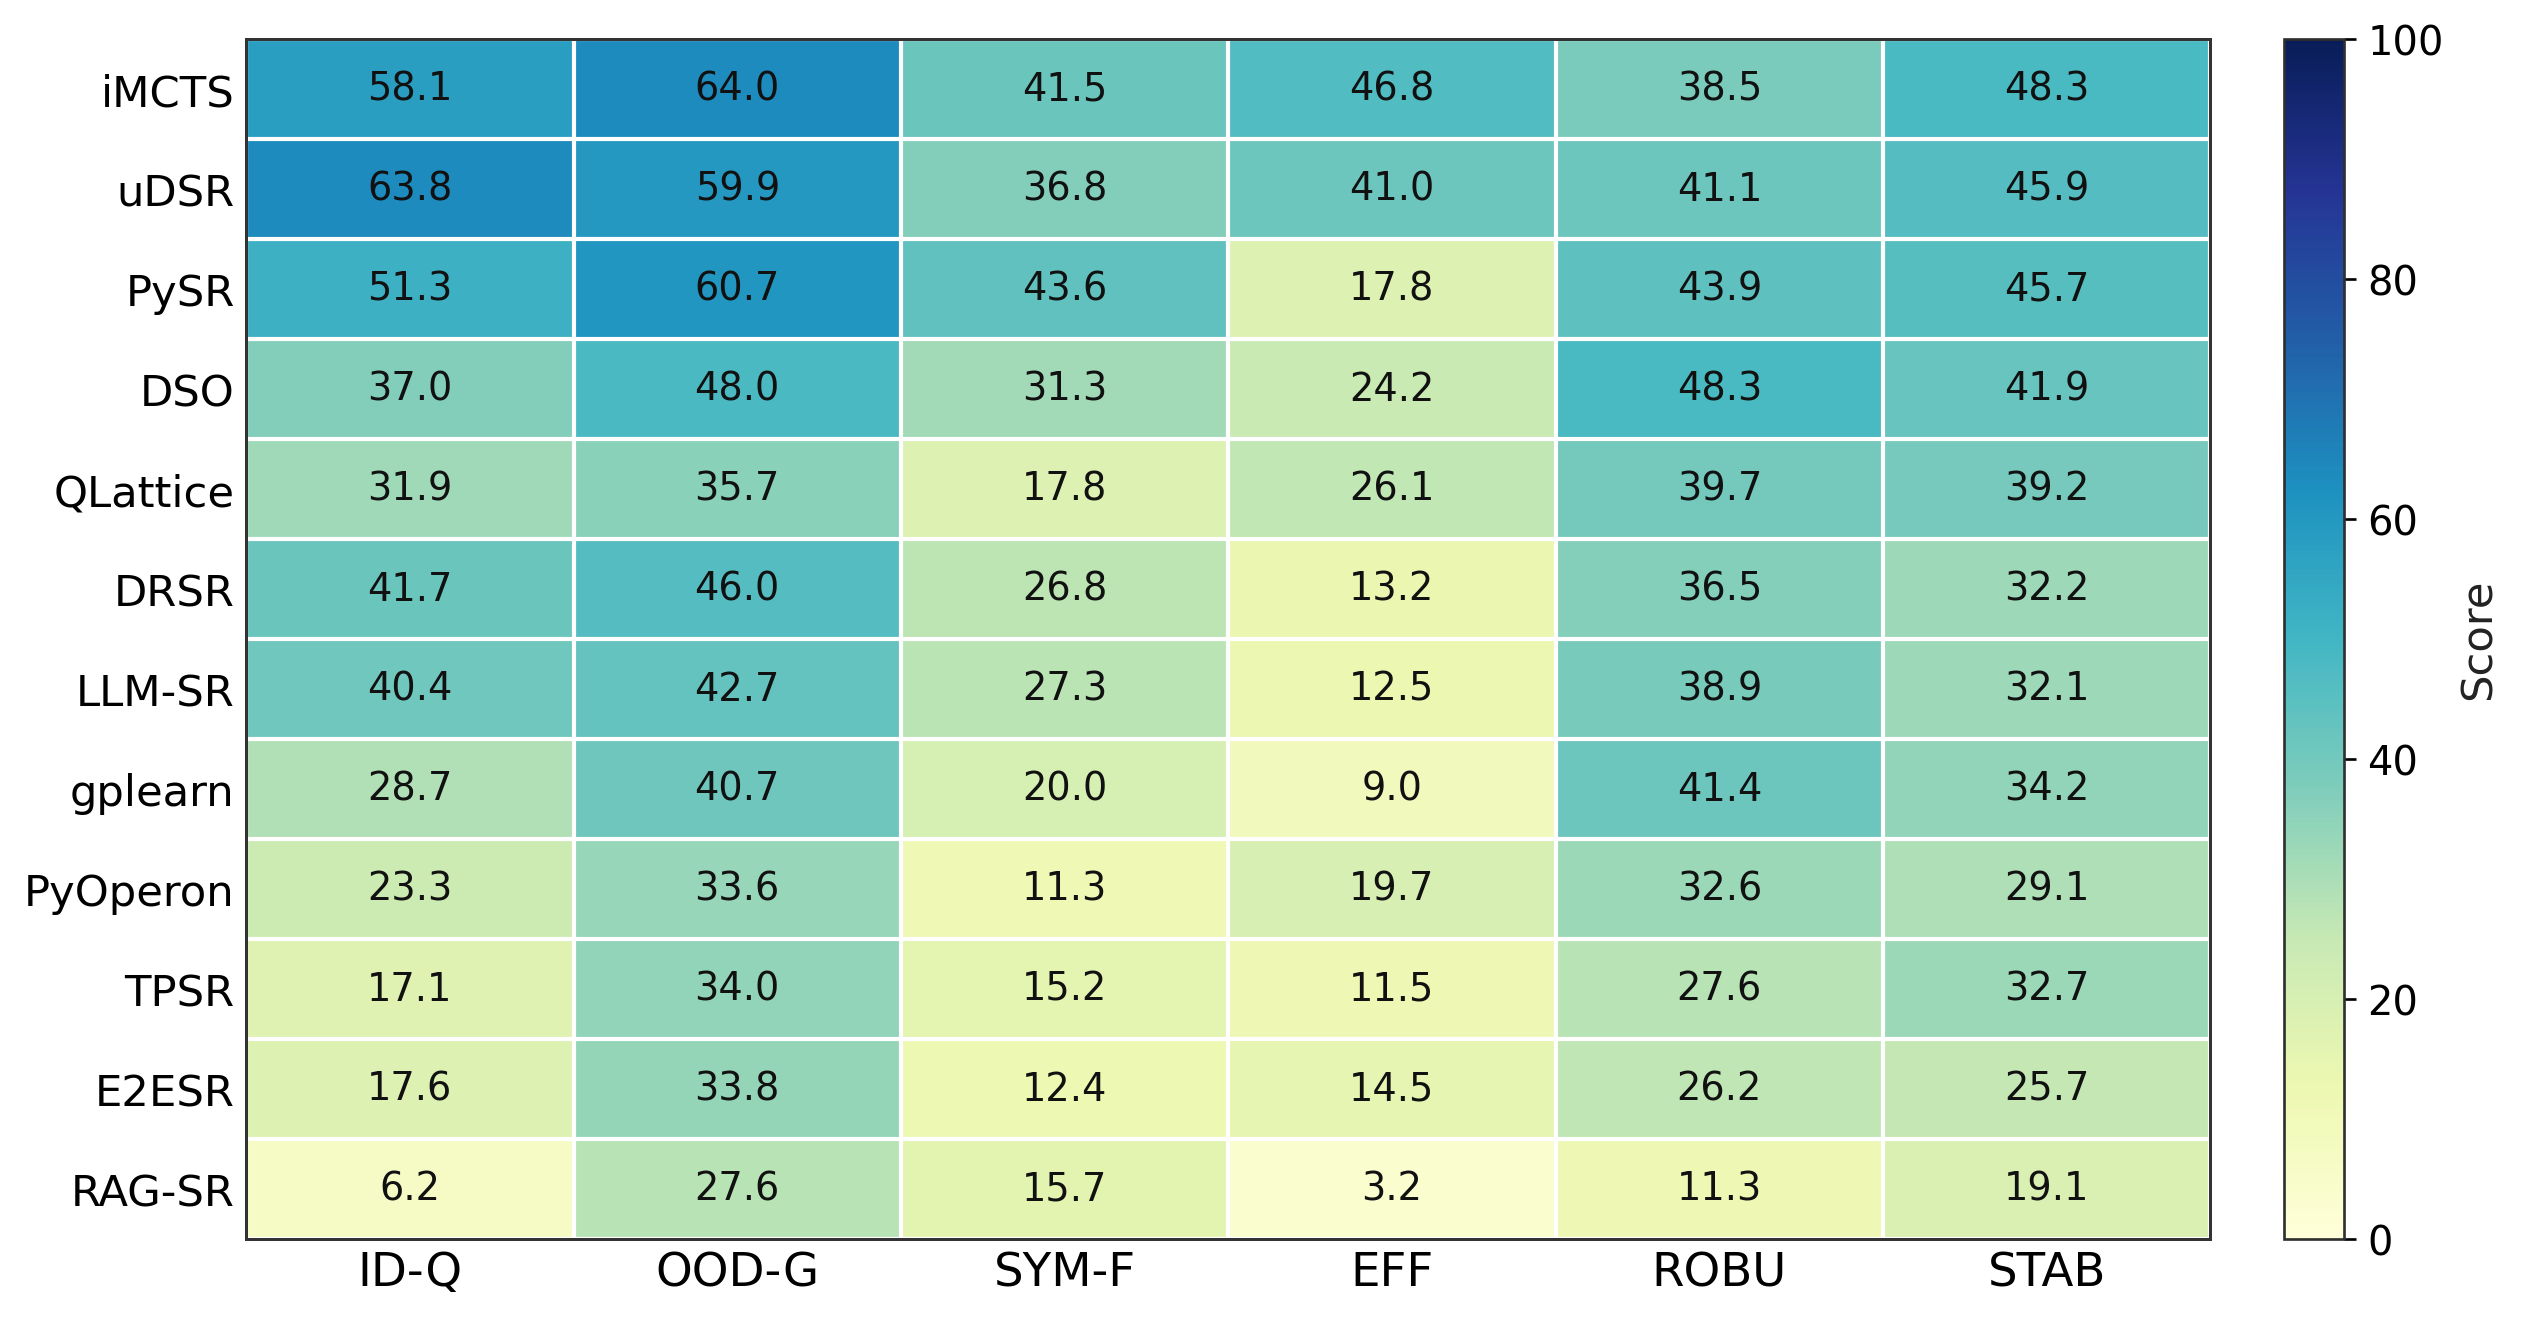
\includegraphics[width=0.90\linewidth]{imgs/Article/figure15_hexagon_heatmap_formal}
\caption{\textbf{Formal clean-track leaderboard heatmap on \core{}.} The heatmap reports \idq{}, \oodg{}, \symf{}, \eff{}, and \stab{}, while \rob{} is marked as a noisy-training extension. It shows that OOD ranking alone does not explain differences in symbolic fidelity, efficiency, and stability.}
\label{fig:hexagon-heatmap}
\end{figure}

\subsection{Dynamic traces and hexagonal evaluation}

The leaderboard protocol records best-so-far expressions every minute, yielding $3000\times60=180000$ search snapshots for the clean \core{} track. Because the trace archive is large, it is packaged as a separate compressed artifact rather than expanded in the paper repository. These traces support time-to-threshold, anytime AUC, complexity-over-time, stagnation, and symbolic-similarity analyses. The clean-track leaderboard reports \idq{}, \oodg{}, \symf{}, \eff{}, and \stab{}; \rob{} is reported only when the shared noisy-training protocol has been completed. The noisy-training robustness curves and heatmap are reported in \cref{app:additional-figures}, because \rob{} is an extension track rather than part of the completed clean-track leaderboard.

\section{Artifact, Documentation, and Reproducibility}

The \arena{} artifact is organized as an anonymized evaluation package rather than only a paper supplement. It includes the standardized dataset lists, algorithm execution assets, result schemas, postprocessing scripts, and reproducibility documentation needed to audit the benchmark construction and leaderboard.

\paragraph{Released components.}
The submission package contains the following components:
\begin{verbatim}
1. Core-50 dataset manifest and dataset files
2. GT-Reservoir-664 metadata
3. Candidate-200 metadata
4. Probe-2 and Probe-4 run summaries
5. Core-50 12-algorithm clean final results
6. Remote-collected minute-level snapshot archive
7. Expression canonicalization and replay utilities
8. Six-axis metric computation scripts
9. Reproduction scripts for Core-50 and leaderboard runs
10. Croissant metadata, dataset card, benchmark card, and license table
\end{verbatim}

The final-result summaries are kept in the main artifact tree. The 180,000 minute-level snapshots are released as a separate compressed trace archive because expanding every progress file substantially increases artifact size.

\paragraph{Result schemas.}
Each run-level artifact records the dataset identifier, algorithm, seed, status, failure reason, wall-clock time, final expression, expression complexity, and train/validation/ID/OOD metrics. Timeout with recovered output is distinguished from timeout without output, so budget exhaustion is not automatically treated as algorithm failure.

\paragraph{Reproduction commands.}
The benchmark is reproducible at three levels: dataset validation, single-run replay, and full-batch scheduling. The minimal reproduction path is:
\begin{verbatim}
python scripts/validate_datasets.py --manifest metadata/core50.csv
python scripts/run_one.py --algorithm pysr --dataset <dataset> --seed 0
python scripts/reproduce_leaderboard.py --manifest metadata/core50.csv
\end{verbatim}
The full cluster schedule used for the reported runs is included separately because the 12-algorithm leaderboard requires heterogeneous CPU and LLM-backed environments. Additional implementation and data-cleaning details are summarized in \cref{app:infra-cleaning}.

\paragraph{Metadata, licenses, and anonymity.}
We provide machine-readable Croissant metadata for the \core{} benchmark and reservoir manifests. For each source benchmark and algorithm wrapper, the artifact records the original source URL, license, and redistribution status. For double-blind review, the released archive removes author-identifying paths and repository names while preserving stable dataset and run identifiers.

\paragraph{Current limitations of the artifact.}
The clean \core{} final results, minute-level trace archive, Probe4-Full postprocessing, and formal symbolic-fidelity artifacts are present in the release package. The ROBU noisy-training track remains an extension: if the paper reports a completed six-axis leaderboard, the shared noisy-training protocol must be regenerated and released with the same result schema.

\section{Limitations}

First, \core{} is a distilled benchmark rather than a replacement for the full 664-task reservoir. It is intended for rapid comparison and development, while full-reservoir evaluation remains useful for final audits.

Second, probe-based selection depends on the selected probe algorithms. \arena{} mitigates this with panel fidelity and complementarity, but future algorithm paradigms may require updating the probe set.

Third, the ground-truth focus favors equation-discovery evaluation. Real-world black-box regression tasks without known formulas are not the primary focus of \arena{}.

Fourth, LLM-assisted methods may benefit from external priors. \arena{} partially controls this by separating no-context probe evaluation from context-enabled full evaluation, but contamination and memorization remain important concerns.

Fifth, ROBU requires additional noisy-training runs. The robustness axis is meaningful only when all submitted algorithms run the same noisy-training protocol.

Finally, symbolic equivalence is imperfect. CAS simplification and numeric equivalence checks can fail on pathological expressions, so thresholds, probe domains, and failure cases must be documented.

\section{Conclusion}

We introduced \arena{}, a unified infrastructure for symbolic regression evaluation. \arena{} addresses two practical bottlenecks in modern SR research: fragmentation of benchmarks and the computational cost of repeated evaluation during algorithm development. By distilling a 664-task ground-truth reservoir into \core{} through cascaded probe-based selection, \arena{} provides a compact benchmark that preserves structural diversity, algorithmic behavior diversity, discriminability, stability, and family coverage. By combining \core{} with unified algorithm execution, minute-level expression logging, canonical expression trees, and a fixed hexagonal metric protocol with clean-track axes and a robustness extension, \arena{} turns symbolic regression benchmarking into a dynamic, interpretable, and extensible evaluation process. We hope \arena{} will support faster iteration, fairer comparison, and deeper analysis of future SR systems across evolutionary, RL, tree-search, neural-guided, and LLM-assisted paradigms.


% Acknowledgments are hidden in anonymized submission mode by the NeurIPS style.
% \begin{ack}
% Acknowledgments and funding disclosures go here for the final version.
% \end{ack}

\bibliographystyle{plainnat}
\bibliography{references}

\newpage
\appendix
\setcounter{figure}{0}
\renewcommand{\thefigure}{A.\arabic{figure}}
\renewcommand{\theHfigure}{appendix.\arabic{figure}}
\section{Related Work}
\label{app:related-work}

\paragraph{Symbolic regression benchmarks.}
Existing SR benchmarks primarily focus on constructing static task collections and reporting final-performance comparisons under a fixed method set. SRBench established one of the first large-scale reproducible evaluation efforts for contemporary symbolic regression, comparing 14 SR methods and 7 machine-learning baselines across 252 regression problems \citep{lacava2021contemporary}. SRSD revisited formula-backed scientific discovery by reconstructing Feynman-style datasets, adding dummy-variable variants, and introducing normalized edit distance for structural expression comparison \citep{matsubara2024rethinking}. LLM-SRBench targets the emerging LLM-based equation-discovery setting with 239 tasks designed to reduce memorization effects and evaluate scientific reasoning beyond common formulas \citep{shojaee2025llmsrbench}. These resources provide important task pools and evaluation conventions. However, they are still largely static benchmark suites: they do not specify how to distill a large heterogeneous reservoir into a compact core benchmark, how to keep scores stable as new algorithms are added, or how to audit search dynamics through intermediate expressions. \arena{} builds on these benchmark resources, but shifts the focus from dataset collection to evaluation infrastructure.

\paragraph{Limitations of static SR evaluation.}
Most existing SR evaluations report final numerical metrics such as MSE, NMSE, or $R^2$ after a fixed search budget \citep{lacava2021contemporary,matsubara2024rethinking,shojaee2025llmsrbench}. This protocol is useful for one-time comparison, but it misses several properties that are central to modern SR systems. First, low numerical error does not necessarily imply symbolic correctness: a method can fit the test region with a non-equivalent shortcut expression. Second, final metrics hide search dynamics: two algorithms with the same final NMSE may differ substantially in time-to-discovery, early-stage quality, or complexity growth. Third, static benchmark tables do not provide stable scores under leaderboard growth if scores are rank-normalized or computed relative to the current method pool. Adjacent evaluation-infrastructure work has made similar criticisms of static benchmarking in NLP and data-centric AI \citep{kiela2021dynabench,ma2021dynaboard,mazumder2023dataperf}. \arena{} addresses these gaps for SR by logging minute-level best-so-far expressions, canonicalizing outputs into expression trees, and using fixed absolute metrics whose values do not drift when new algorithms are added.

\paragraph{Modern SR algorithms.}
The SR algorithmic landscape has diversified beyond classical genetic programming. Evolutionary and GP-style systems, including PySR, PyOperon, and gplearn, search over expression trees and often combine structure search with constant optimization \citep{cranmer2023pysr}. Physics-inspired systems such as AI Feynman exploit inductive biases including symmetry, separability, and compositional structure to decompose equation discovery into simpler subproblems \citep{udrescu2020aifeynman}. Reinforcement-learning and policy-search approaches, such as DSR, learn expression-generating policies using reward signals derived from numerical fit and expression quality \citep{petersen2021dsr}. Neural-guided and hybrid methods combine learned proposal mechanisms with symbolic search or genetic-programming components \citep{mundhenk2021dsoseeding}. Transformer-based and planning-based systems use pretraining or tree search to guide symbolic generation \citep{shojaee2023tpsr}. More recent LLM-assisted SR systems use language models to propose equation programs, scientific hypotheses, or context-aware symbolic structures \citep{shojaee2025llmsr}. Because these paradigms differ in prior usage, search trajectory, symbolic faithfulness, runtime cost, OOD behavior, and seed stability, a single final-error table is insufficient to characterize them. \arena{} is not a new SR algorithm; it is designed to evaluate this increasingly heterogeneous algorithmic space under one executable contract.

\paragraph{LLM-assisted equation discovery.}
LLM-assisted SR introduces a new evaluation challenge. Unlike traditional symbolic search, LLM-based methods can exploit natural-language descriptions, scientific priors, memorized formula patterns, or prompt-specific reasoning strategies \citep{shojaee2025llmsr,shojaee2025llmsrbench}. This makes direct comparison with non-LLM systems difficult unless the evaluation protocol explicitly controls what contextual information is provided. LLM-oriented benchmarks therefore emphasize anti-memorization design and scientific equation-discovery tasks \citep{shojaee2025llmsrbench}. \arena{} separates these concerns in two ways. First, PySR and LLM-SR are used as dual probes without physical background information during \candidate{} mining, so the initial high-information pool is not merely a test of language-context advantage. Second, LLM-assisted methods can still participate in the formal leaderboard, but their context usage and prompt contract are explicitly recorded. This separation allows \arena{} to use LLM systems as informative probes without letting LLM priors dominate the construction of the final \core{}.

\paragraph{Benchmark distillation and core-set selection.}
Large benchmark suites improve coverage, but their cost makes them difficult to use during iterative algorithm development. A common workaround is to evaluate on a smaller subset, but naive random sampling, family-stratified sampling, or difficulty-only selection can miss the behavioral conclusions induced by the full method panel. Recent work on efficient model evaluation and benchmark subset selection argues that smaller benchmarks should preserve more than item diversity: they should also preserve method ranking, item discrimination, and distributional coverage \citep{perlitz2024efficient,polo2024tinybenchmarks,vivek2024anchorpoints,saranathan2025sublime}. \arena{} treats subset construction as benchmark distillation rather than convenience sampling. Its \core{} objective jointly considers structural coverage, response-space coverage, method discriminability, redundancy control, difficulty and failure-mode balance, and seed-level stability. This differs from selecting the easiest, hardest, or largest-gap tasks. It also differs from metadata-only core-set selection because \arena{} uses probe-algorithm responses to preserve behavioral conclusions from the larger 664-task reservoir.

\paragraph{Probe-based evaluation and algorithm-panel fidelity.}
A key challenge in benchmark distillation is that the selected subset should represent not only the task distribution, but also the conclusions that a larger algorithm panel would induce. \arena{} addresses this through a cascaded probe design. First, PySR and LLM-SR are used as dual probes to mine a high-information \candidate{} pool, intentionally exposing differences between a strong traditional SR system and an LLM-assisted paradigm. Second, \arena{} evaluates 12 integrated algorithms on \candidate{} and selects four non-LLM probes through a health-gated exhaustive subset-selection procedure. The selected \probe{} is optimized for health, panel fidelity, behavioral complementarity, and dataset coverage rather than average performance alone. This probe-selection step is important because the final \core{} is not chosen to favor the strongest algorithms; it is chosen to approximate the dataset-informativeness judgments of a broader algorithm panel while remaining computationally tractable.

\paragraph{Expression-level evaluation.}
Several SR benchmarks recognize that numerical error alone is insufficient for scientific discovery. SRSD, for example, introduced normalized edit distance to compare predicted expressions with ground-truth formulas \citep{matsubara2024rethinking}. This is important because symbolic regression is often used not merely to predict values, but to recover interpretable mechanisms. \arena{} extends expression-level evaluation in two directions. First, all outputs are canonicalized into a common expression-tree representation, allowing equivalence testing, tree similarity, variable recovery, operator recovery, and seed-level structural consistency. Second, symbolic fidelity is integrated into the leaderboard as a first-class axis rather than treated as a post-hoc diagnostic. This makes it possible to distinguish low-NMSE equivalent formulas from low-NMSE but symbolically incorrect shortcuts.

\paragraph{OOD generalization and robustness in SR.}
OOD behavior is central to equation discovery because a formula that only interpolates the training domain may not reflect the underlying mechanism. Prior SR benchmarks have considered extrapolation or scientific-discovery splits to varying degrees \citep{lacava2021contemporary,matsubara2024rethinking,shojaee2025llmsrbench}. However, OOD evaluation is often reported as another final-error column, without explicitly separating absolute OOD quality from ID-to-OOD degradation. \arena{} defines \oodg{} as a combination of OOD quality and ID-to-OOD retention, preventing methods from being rewarded simply because they perform poorly both in and out of distribution. \arena{} further defines \rob{} as a noisy-training extension track, measuring whether algorithms trained on corrupted labels can still recover clean ID/OOD behavior. This separates clean-track evaluation from robustness evaluation while keeping both under a shared metric protocol.

\paragraph{Efficiency, anytime behavior, and search traces.}
SR methods can differ substantially in how quickly they discover useful expressions. Evolutionary systems may gradually improve over time, neural-guided systems may find strong candidates early, and LLM-assisted systems may generate high-quality initial structures but vary in refinement behavior. Existing SR benchmarks typically report final scores after a fixed budget, which hides these anytime differences. Dynamic benchmarking and evaluation-as-a-service work in other domains has argued for richer evaluation artifacts, stable infrastructure, and additional metrics beyond accuracy \citep{kiela2021dynabench,ma2021dynaboard}. \arena{} brings this idea to SR by recording best-so-far expressions every minute under a shared one-hour budget, enabling efficiency metrics based on quality-time AUC, time-to-threshold, stagnation analysis, and complexity-over-time. This turns the leaderboard from a final-score table into a diagnostic tool for understanding search behavior.

\paragraph{Evaluation infrastructure and dataset documentation.}
Recent evaluation practice increasingly emphasizes not only benchmark results, but also artifact documentation, dataset cards, model cards, data statements, metadata, and reproducibility pathways \citep{gebru2021datasheets,mitchell2019modelcards,bender2018datastatements,pushkarna2022datacards,akhtar2024croissant}. Data-centric evaluation efforts such as DataPerf also argue that benchmark infrastructures should support iterative development and long-term maintenance rather than one-off static comparisons \citep{mazumder2023dataperf}. \arena{} follows this direction by releasing dataset manifests, standardized result schemas, expression canonicalization tools, metric-computation scripts, license tables, and Croissant-style metadata. Its contribution is therefore not only the \core{} task set, but the infrastructure connecting task standardization, algorithm wrappers, result semantics, benchmark distillation, dynamic leaderboard updates, and expression-level diagnostics. In this sense, \arena{} aims to make SR benchmarking auditable and extensible rather than merely rank-based.


\clearpage
\setcounter{figure}{0}
\renewcommand{\thefigure}{B.\arabic{figure}}
\renewcommand{\theHfigure}{appendixB.\arabic{figure}}
% \section{\core{} Selection Details}
% \label{app:core50-details}

% This appendix gives the full selection definitions behind the simplified objective in the main text. The purpose is reproducibility: the main paper explains why the distillation path is reasonable, while this appendix specifies how the scoring terms, constraints, and audits are computed.

% \subsection{Candidate-200 selection audit}

% Candidate-200 is constructed as a calibration pool after the dual-probe stage. Let $\ell_{i,a}^{id}$ and $\ell_{i,a}^{ood}$ denote clipped log-NMSE for dataset $i$ and algorithm $a$. The two-probe disagreement features are
% \[
% g_i^{id}=\ell_{i,\mathrm{LLMSR}}^{id}-\ell_{i,\mathrm{PySR}}^{id},\qquad
% g_i^{ood}=\ell_{i,\mathrm{LLMSR}}^{ood}-\ell_{i,\mathrm{PySR}}^{ood},
% \]
% \[
% G_i=\frac{|g_i^{id}|+|g_i^{ood}|}{2}.
% \]
% Positive gaps indicate PySR advantage and negative gaps indicate LLM-SR advantage. Candidate-200 is selected from high-$G_i$ tasks, one-sided evaluability tasks, and mid-gap tasks under source-family, subgroup, basename, and advantage-side caps. \Cref{tab:candidate200-selection-audit} reports the realized selection modes.

% \begin{table}[ht]
% \centering
% \small
% \caption{Candidate-200 selection modes. The candidate pool is intentionally high-information rather than a random miniature of \reservoir{}.}
% \label{tab:candidate200-selection-audit}
% \begin{tabular}{llrr}
% \toprule
% Pool & Selection mode & \#Datasets & Mean gap \\
% \midrule
% A & strict high-disagreement & 126 & 31.302 \\
% A & relaxed high-disagreement & 14 & 0.259 \\
% B & one-sided evaluability & 20 & -- \\
% C & mid-gap & 40 & 14.331 \\
% \bottomrule
% \end{tabular}
% \end{table}

% \subsection{Probe-4 selection details}

% The 12-method Candidate-200 calibration stage is summarized at the method level by finite ID/OOD rate, explosion rate, operational stability, discrimination, and dataset coverage. Non-LLM probe candidates are first filtered by execution health, then all feasible four-method panels are scored by
% \[
% \mathrm{Score}(P)=0.20H(P)+0.40F(P)+0.25C(P)+0.15V(P).
% \]
% $H(P)$ averages execution health; $F(P)$ measures how well the panel preserves dataset-informativeness judgments from the larger method panel; $C(P)$ rewards response-space complementarity; and $V(P)$ rewards family/subgroup/difficulty coverage. The final decision also applies taxonomy constraints and excludes methods whose construction role is already used in dual-probe mining or whose behavior depends on LLM/RAG context. This is why the final selected panel is not the NMSE-only top-ranked set.

% \begin{table}[ht]
% \centering
% \small
% \caption{Candidate-200 algorithm health metrics used before Probe-4 subset selection.}
% \label{tab:probe4-health-audit}
% \begin{tabular}{llrrrr}
% \toprule
% Algorithm & Taxonomy & Finite rate & Explosion rate & Stability & Score \\
% \midrule
% PySR & evolutionary-GP & 0.985 & 0.205 & 0.973 & 0.600 \\
% iMCTS & MCTS & 0.990 & 0.055 & 0.990 & 0.481 \\
% uDSR & RL-hybrid & 0.990 & 0.015 & 0.990 & 0.469 \\
% gplearn & classic-GP & 1.000 & 0.140 & 1.000 & 0.449 \\
% TPSR & pretrained-neural & 0.975 & 0.250 & 0.975 & 0.448 \\
% DSO & RL-policy & 0.990 & 0.050 & 0.990 & 0.441 \\
% RAG-SR & RAG-hybrid & 0.885 & 0.585 & 0.885 & 0.415 \\
% PyOperon & evolutionary-GP & 0.975 & 0.035 & 0.967 & 0.369 \\
% E2ESR & pretrained-neural & 0.695 & 0.140 & 0.695 & 0.366 \\
% QLattice & graph-hybrid & 0.950 & 0.030 & 0.950 & 0.361 \\
% \bottomrule
% \end{tabular}
% \end{table}

% \begin{table}[ht]
% \centering
% \small
% \caption{Probe-4 subset audit. The final selected panel is reported alongside the NMSE-only high-scoring panels to make the taxonomy-aware decision explicit.}
% \label{tab:probe4-combination-audit}
% \begin{tabular}{rlrrl}
% \toprule
% NMSE-only rank & Probe combination & Score & Finite rate & Selection note \\
% \midrule
% 1 & iMCTS; PySR; RAG-SR; uDSR & 0.790 & 0.963 & NMSE-only high score \\
% 2 & iMCTS; PySR; RAG-SR; TPSR & 0.783 & 0.959 & NMSE-only high score \\
% 3 & PySR; RAG-SR; TPSR; uDSR & 0.781 & 0.959 & NMSE-only high score \\
% 4 & gplearn; iMCTS; PySR; RAG-SR & 0.773 & 0.965 & NMSE-only high score \\
% 5 & gplearn; PySR; RAG-SR; uDSR & 0.772 & 0.965 & NMSE-only high score \\
% 150 & DSO; iMCTS; PyOperon; uDSR & 0.667 & 0.986 & final selected \\
% \bottomrule
% \end{tabular}
% \end{table}

% \subsection{Run-level cleaning and aggregation}

% Unfinished runs are not treated as invalid runs. A run first receives an outcome class:
% \begin{gather*}
% \{\texttt{valid\_finite},\texttt{valid\_extreme},\texttt{partial},
% \texttt{timeout\_no\_output},\\
% \texttt{invalid},\texttt{system\_error},\texttt{not\_finished}\}.
% \end{gather*}
% Only finished runs with the correct dataset identity are evaluable. Valid extreme-error runs remain valid; their NMSE values are clipped rather than dropped.

% For every run, raw NMSE is mapped to clipped log space:
% \[
% \ell(x)=\mathrm{clip}\left(\log_{10}(\max(x,10^{-12})),-12,12\right).
% \]
% For dataset $i$, probe $p$, and seed set $\mathcal{S}$, the dataset--probe aggregates are:
% \[
% m_{i,p}^{id}=\mathrm{median}_{s\in\mathcal{S}_{valid}}\ell(\mathrm{NMSE}_{i,p,s}^{id}),\qquad
% m_{i,p}^{ood}=\mathrm{median}_{s\in\mathcal{S}_{valid}}\ell(\mathrm{NMSE}_{i,p,s}^{ood}),
% \]
% \[
% \begin{aligned}
% r_{i,p}&=\frac{|\mathcal{S}_{valid}|}{|\mathcal{S}_{evaluable}|},\\
% q_{i,p}^{id}&=\mathrm{IQR}_{s\in\mathcal{S}_{valid}}\ell(\mathrm{NMSE}_{i,p,s}^{id}),\\
% q_{i,p}^{ood}&=\mathrm{IQR}_{s\in\mathcal{S}_{valid}}\ell(\mathrm{NMSE}_{i,p,s}^{ood}).
% \end{aligned}
% \]
% If no valid seed is available for a dataset--probe pair, the pair is excluded from performance medians but contributes to invalid and timeout rates.

% \subsection{Robust normalization}

% All continuous selection features use robust min-max normalization:
% \[
% \mathrm{rmin}(x)=P_5(x),\qquad \mathrm{rmax}(x)=P_{95}(x),
% \]
% \[
% \mathrm{Norm}(x)=
% \mathrm{clip}\left(\frac{x-\mathrm{rmin}(x)}{\mathrm{rmax}(x)-\mathrm{rmin}(x)},0,1\right).
% \]
% If $\mathrm{rmax}(x)=\mathrm{rmin}(x)$, the normalized value is set to zero. Robust normalization prevents a small number of catastrophic NMSE explosions from dominating the selection score.

% \subsection{Dataset-level information score}

% For each dataset $i$, the Probe-4 response vector contains median ID/OOD quality, OOD-ID degradation, valid-output pattern, and seed variability. The discrimination score is
% \[
% \begin{aligned}
% \mathrm{Disc}_i={}&
% 0.35\,\mathrm{Norm}\!\left(\mathrm{Var}_{p}(m_{i,p}^{id})\right)
% +0.35\,\mathrm{Norm}\!\left(\mathrm{Var}_{p}(m_{i,p}^{ood})\right)\\
% &+0.15\,\mathrm{Norm}\!\left(\mathrm{Var}_{p}(m_{i,p}^{ood}-m_{i,p}^{id})\right)
% +0.10\,\mathrm{Norm}\!\left(\mathrm{Mean}_{p<q}|m_{i,p}^{ood}-m_{i,q}^{ood}|\right)\\
% &+0.05\,\mathrm{Norm}\!\left(H(\mathrm{valid\_pattern}_{i,:})\right).
% \end{aligned}
% \]
% The instability score is
% \[
% \begin{aligned}
% \mathrm{Instab}_i=
% {}&0.40\,\mathrm{Mean}_{p}(q_{i,p}^{ood})
% +0.20\,\mathrm{Mean}_{p}(q_{i,p}^{id})
% +0.20\,\mathrm{Max}_{p}(q_{i,p}^{ood})\\
% &+0.10\,\mathrm{invalid\_rate}_i
% +0.10\,\mathrm{timeout\_rate}_i.
% \end{aligned}
% \]
% The stability and information scores are
% \[
% \mathrm{Stab}_i=1-\mathrm{Norm}(\mathrm{Instab}_i),\qquad
% \mathrm{Info}_i=\mathrm{Disc}_i\cdot \mathrm{Stab}_i.
% \]
% Thus, a dataset receives high information only when it separates probes and the separation is not primarily caused by seed noise, invalid outputs, or timeout artifacts.

% \subsection{Difficulty, failure mode, and eligibility}

% Dataset difficulty is computed from the mean ID/OOD quality across valid probes:
% \[
% \mathrm{Difficulty}_i=
% \mathrm{Mean}_{p}\left[\frac{m_{i,p}^{id}+m_{i,p}^{ood}}{2}\right].
% \]
% Datasets are binned into easy, medium, hard, and extreme by robust quantiles, with high invalid or timeout rates allowed to override the bin to extreme. Failure modes are assigned in priority order: incomplete, invalid-prone, one-sided, unstable, OOD-failure, all-struggle, one-method-wins, and all-good. Eligibility is then one of eligible, limited-quota, excluded, or incomplete. Limited-quota datasets are not discarded; they are allowed to enter \core{} only under caps.

% \subsection{Coverage and balance terms}

% For a categorical attribute $a$, let $\mathcal{C}_a(D)$ be the set of categories observed in the full reservoir and $\mathcal{C}_a(S)$ those observed in a subset. Category coverage is
% \[
% \mathrm{Cov}_a(S)=\frac{|\mathcal{C}_a(S)|}{|\mathcal{C}_a(D)|}.
% \]
% Structural coverage averages coverage over family, subgroup, operator group, feature-count bin, sample-count bin, formula-complexity bin, OOD type, and dummy-variable status. Response coverage averages coverage over difficulty bin, failure mode, winner probe, and valid-output pattern:
% \[
% \mathrm{Coverage}(S)=0.6\,\mathrm{StructuralCoverage}(S)+0.4\,\mathrm{ResponseCoverage}(S).
% \]
% Balance measures distributional similarity to the full reservoir. For categorical attribute $a$, let $p_a^S$ and $p_a^D$ be empirical distributions in the subset and the full reservoir. We use total-variation similarity:
% \[
% \mathrm{Sim}_a(S,D)=1-\frac{1}{2}\sum_{c}|p_a^S(c)-p_a^D(c)|.
% \]
% The balance term is a weighted average of $\mathrm{Sim}_a$ over the same structural and response-derived bins.

% \subsection{Full subset objective and hard constraints}

% The full subset score is
% \[
% J(S)=0.45\,\mathrm{Coverage}(S)+0.35\,\frac{1}{|S|}\sum_{i\in S}\mathrm{Info}_i+0.20\,\mathrm{Balance}(S),
% \]
% subject to:
% \[
% |S|=50.
% \]
% The objective is optimized only over feasible subsets. The main hard constraints are:
% \begin{itemize}[leftmargin=*]
%     \item semantic duplicate cap: each semantic duplicate group appears at most once;
%     \item basename cap: no repeated basename in the released \core{} manifest;
%     \item family quota: each family $f$ receives a smoothed quota derived from reservoir frequency,
%     \[
%     t_f=0.6\frac{n_f}{664}+0.4\frac{1}{F},\qquad
%     q_f^{target}=50t_f,
%     \]
%     \[
%     q_f^{min}=\max(1,\lfloor q_f^{target}-1\rfloor),\qquad
%     q_f^{max}=\lceil q_f^{target}+2\rceil;
%     \]
%     \item subgroup concentration cap: no subgroup can dominate the selected subset;
%     \item difficulty quota: easy, medium, hard, and extreme tasks must all be represented;
%     \item limited-quota caps: invalid-prone, one-sided, unstable, and extreme cases are allowed but capped;
%     \item materialization audit: result-derived columns are removed from the released manifest.
% \end{itemize}
% The realized \core{} family counts are 16 LLM-SRBench, 15 SRSD, 9 SRBench 1.0, 3 Nguyen, 2 SRBench2025, 2 Korns, 2 Keijzer, and 1 Vladislavleva. Each selected basename appears once.

% \subsection{Search procedure}

% Selection is implemented as constrained local search:
% \begin{enumerate}[leftmargin=*]
%     \item construct an initial feasible subset using family quotas and high-information eligible datasets;
%     \item repair hard-constraint violations, especially duplicates and over-concentrated subgroups;
%     \item evaluate $J(S)$ for the feasible subset;
%     \item repeatedly propose one-for-one swaps that preserve feasibility;
%     \item accept swaps that improve $J(S)$;
%     \item run multiple random restarts and retain the highest-scoring feasible subset;
%     \item export the frozen manifest and a selection audit report.
% \end{enumerate}
% This procedure is deliberately auditable rather than opaque: the released artifact records the input dataset-level table, selection scores, selected manifest, and post-selection balance report.

% \subsection{Baseline subset definitions}

% We compare \core{} with several 50-task alternatives:
% \begin{itemize}[leftmargin=*]
%     \item \textbf{random-50}: uniformly sampled 50-task subsets;
%     \item \textbf{family-stratified random-50}: random subsets sampled approximately proportional to family sizes;
%     \item \textbf{top-info-50}: top 50 datasets by $\mathrm{Info}_i$;
%     \item \textbf{metadata-diverse-50}: metadata-only diverse subset using feature count, formula complexity, sample count, and family coverage;
%     \item \textbf{difficulty-balanced-50}: quota-balanced subset over difficulty bins, with high-information tie-breaks.
% \end{itemize}
% \Cref{tab:core50-baseline-quality-audit} reports the subset-quality summary used for the radar plot in the main text. Some columns are quality scores where higher is better; the rank-fidelity comparison additionally reports $1-\mathrm{aggregate\ error}$ in the generated figure.

% \begin{table}[ht]
% \centering
% \small
% \caption{Subset-quality summary for \core{} and alternative 50-task selectors. Higher is better for all columns shown here.}
% \label{tab:core50-baseline-quality-audit}
% \resizebox{\linewidth}{!}{%
% \begin{tabular}{lrrrrrr}
% \toprule
% Subset & Coverage & Mean info & Rank fidelity & Stability & Non-red. & Diff. balance \\
% \midrule
% \core{} & 0.838 & 0.471 & 1.000 & 0.835 & 0.769 & 0.892 \\
% top-info-50 & 0.784 & 0.691 & 1.000 & 0.911 & 0.860 & 0.780 \\
% metadata-diverse-50 & 0.635 & 0.085 & 1.000 & 0.735 & 0.860 & 0.601 \\
% difficulty-balanced-50 & 0.817 & 0.637 & 1.000 & 0.883 & 0.920 & 0.999 \\
% random-50 avg & 0.835 & 0.187 & 0.983 & 0.705 & 0.970 & 0.908 \\
% family-stratified random-50 avg & 0.815 & 0.191 & 0.995 & 0.696 & 0.968 & 0.909 \\
% \bottomrule
% \end{tabular}
% }
% \end{table}
\section{\core{} Distillation Details}
\label{app:core50-details}

This appendix provides the full selection definitions behind the simplified \core{} distillation procedure in the main text. The purpose of this appendix is reproducibility and auditability: the main paper explains the rationale of the cascaded distillation path, while this appendix specifies how the scoring terms, constraints, subset baselines, and construction audits are computed.

\subsection{Candidate-200 Selection Audit}
\label{app:candidate200-audit}

Candidate-200 is constructed as a high-information calibration pool after the dual-probe mining stage. The two probes are PySR and LLM-SR, each run once on all 664 ground-truth datasets:$664 \times 2 = 1328.$
%Physical background descriptions are withheld during this stage, so the LLM-based probe cannot directly exploit semantic context.

Let \(\ell_{i,a}^{id}\) and \(\ell_{i,a}^{ood}\) denote clipped log-NMSE for dataset \(i\) and algorithm \(a\) on the ID and OOD test splits. The two-probe disagreement features are
\[
g_i^{id}
=
\ell_{i,\mathrm{LLMSR}}^{id}
-
\ell_{i,\mathrm{PySR}}^{id},
\qquad
g_i^{ood}
=
\ell_{i,\mathrm{LLMSR}}^{ood}
-
\ell_{i,\mathrm{PySR}}^{ood},
\]
and the overall disagreement score is
\[
G_i
=
\frac{
|g_i^{id}|
+
|g_i^{ood}|
}{2},
\]
 here positive gaps indicate PySR advantage, while negative gaps indicate LLM-SR advantage.

Candidate-200 combines high-disagreement tasks, one-sided evaluability cases, and mid-gap tasks under source-family, subgroup, basename, and advantage-side caps. The resulting pool is therefore a calibration set designed to expose method differences and failure modes rather than a random miniature of \reservoir{}.

\begin{table}[ht]
\centering
\small
\caption{\textbf{Candidate-200 selection modes.}}
\label{tab:candidate200-selection-audit}
\begin{tabular}{llrr}
\toprule
\textbf{Pool} & \textbf{Selection mode} & \textbf{\#Datasets} & \textbf{Mean gap} \\
\midrule
A & strict high-disagreement & 126 & 31.302 \\
A & relaxed high-disagreement & 14 & 0.259 \\
B & one-sided evaluability & 20 & -- \\
C & mid-gap & 40 & 14.331 \\
\bottomrule
\end{tabular}
\end{table}

As shown in \Cref{tab:candidate200-selection-audit}, the realized label distribution is 126\ $\mathrm{strict}$,
14\ $\mathrm{relaxed}$,
20\ $\mathrm{one\mbox{-}sided}$,
40\ $\mathrm{mid\mbox{-}gap}$.
The realized family distribution is:
\[
70\ \mathrm{SRSD},
\quad
70\ \mathrm{LLM\mbox{-}SRBench},
\quad
33\ \mathrm{SRBench1.0},
\]
\[
9\ \mathrm{Korns},
\quad
6\ \mathrm{Keijzer},
\quad
6\ \mathrm{Nguyen},
\quad
6\ \mathrm{SRBench2025}.
\]
\Cref{fig:dual-probe-scatter} shows PySR/LLM-SR disagreement on ID and OOD splits. Selected Candidate-200 tasks are concentrated in off-diagonal or asymmetric regions, indicating that the dual-probe stage captures datasets with informative method differences rather than simply sampling the reservoir at random.
\begin{figure}[ht]
\centering
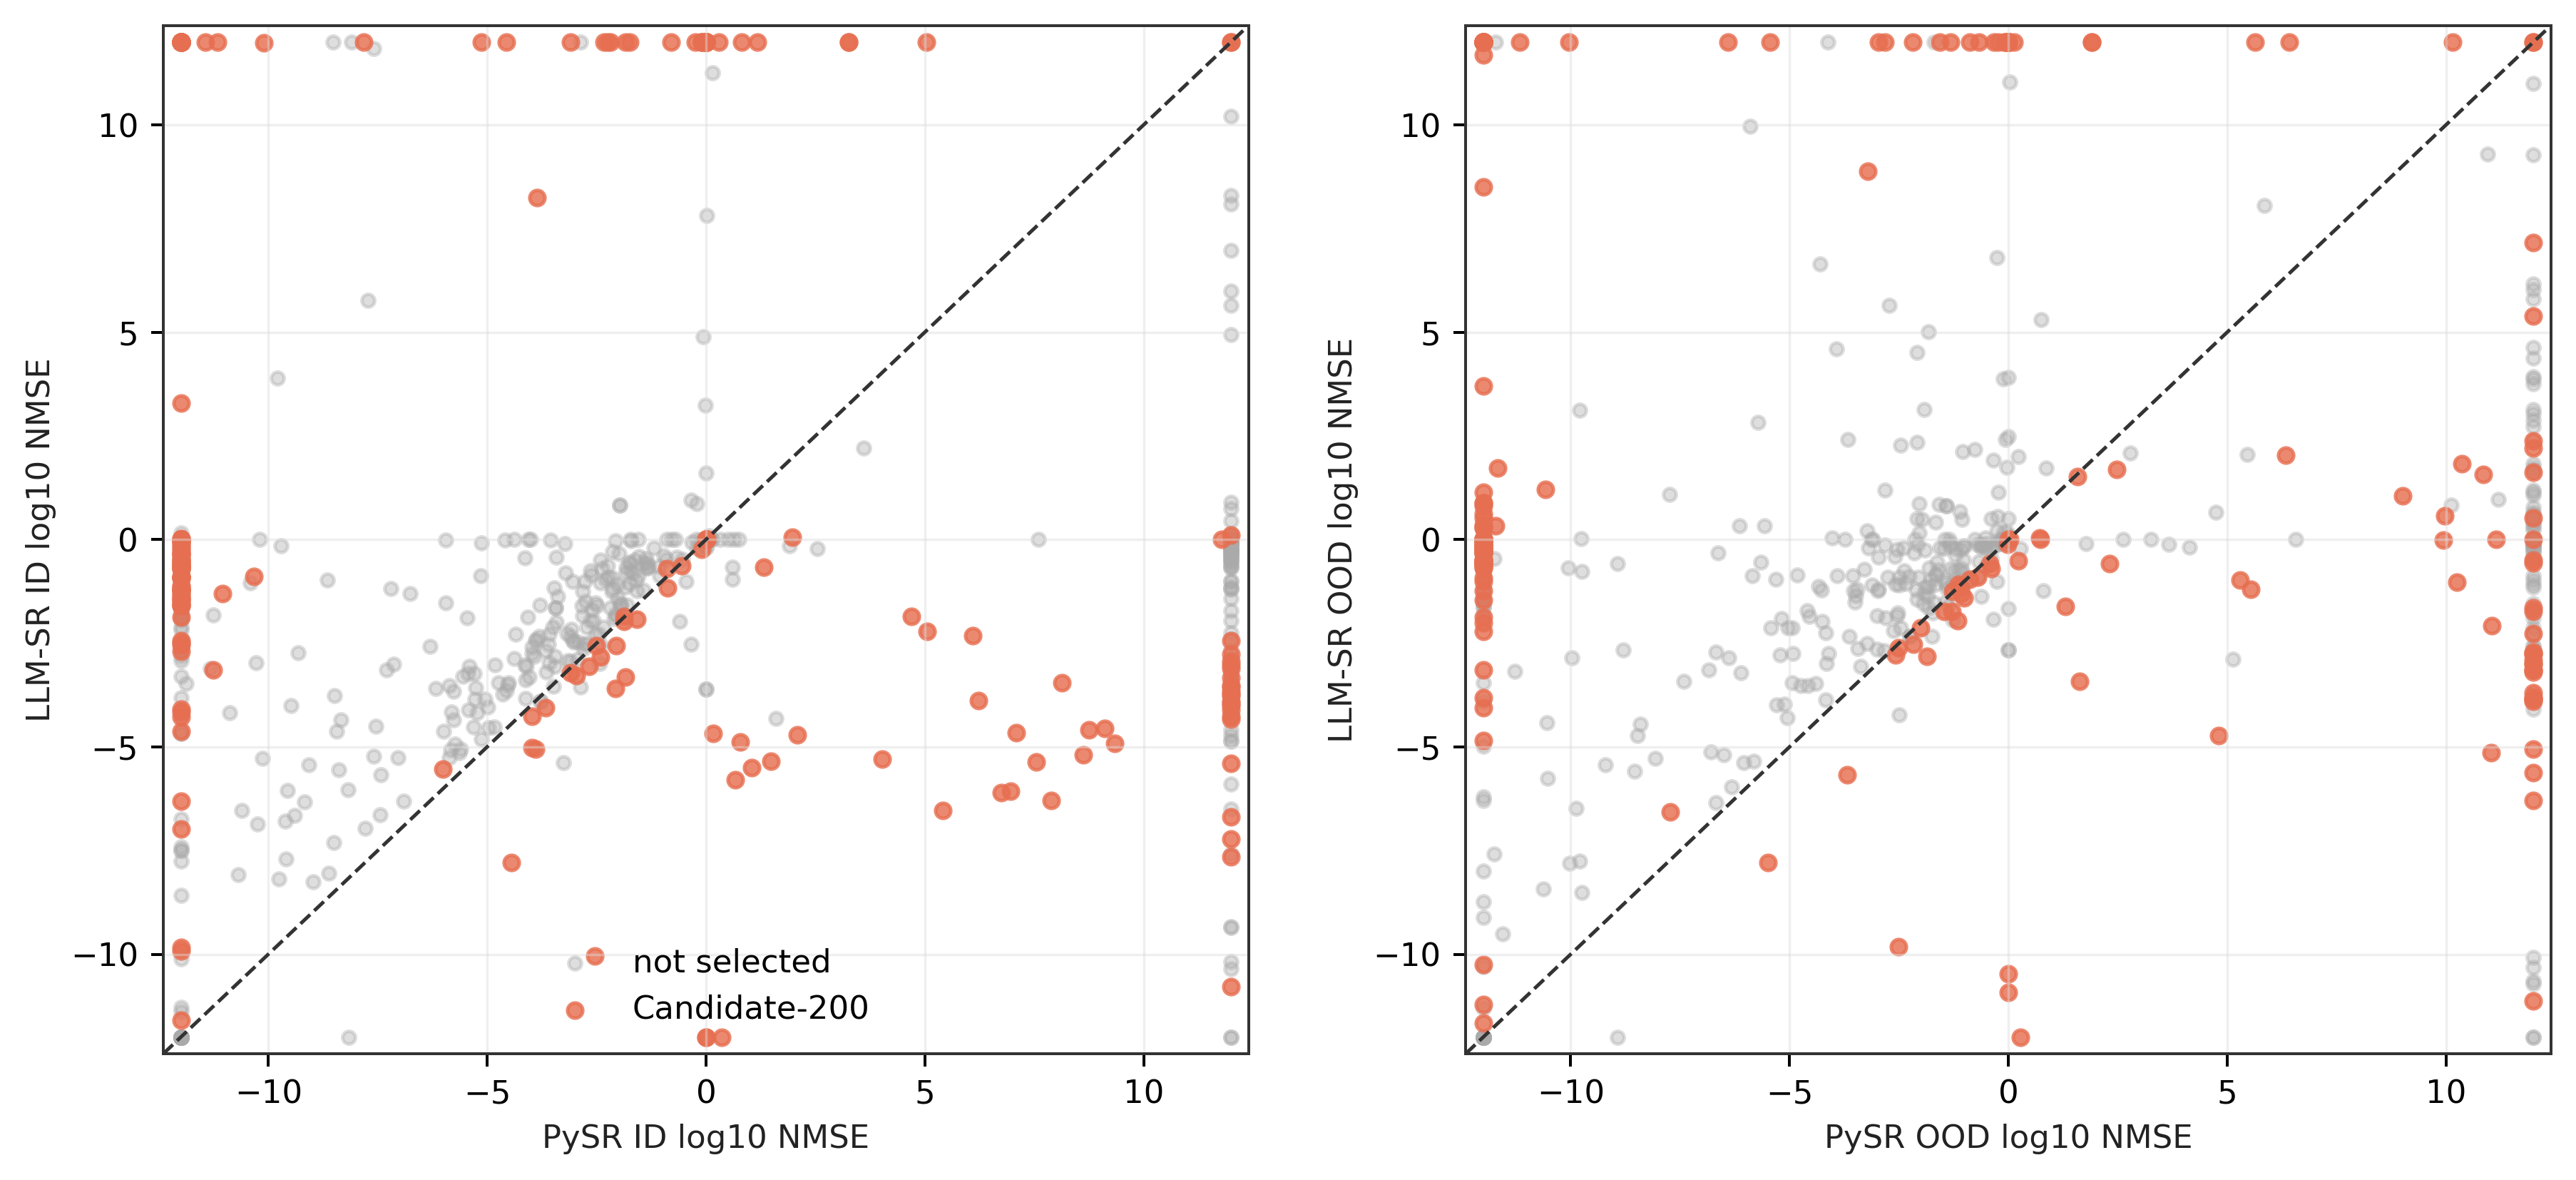
\includegraphics[width=0.68\linewidth]{imgs/Appendix/figure03_dual_probe_scatter}
\caption{\textbf{Dual-probe mining diagnostic.} Each point is a dataset, with PySR and LLM-SR log-NMSE shown on the two axes. Off-diagonal points indicate strong probe disagreement; selected Candidate-200 tasks cover these informative regions on both ID and OOD splits.}
\label{fig:dual-probe-scatter}
\end{figure}


\subsection{Probe-4 Selection Details}
\label{app:probe4-selection}

The Probe-4 selection stage uses the 12-method calibration results on Candidate-200.%: $200 \times 12 = 2400$ single-seed runs. 
Each run provides train, ID, and OOD NMSE values, together with validity and failure status.

\paragraph{Health gate.}
An algorithm \(a\) enters the probe candidate pool only if it satisfies:
\[
\mathrm{finite}(a)\ge 0.90,
\qquad
\mathrm{explode}(a)\le 0.25,
\]
The finite-result rate is
\[
\mathrm{finite}(a)
=
\frac{
\#\{d:\mathrm{train},\mathrm{ID},\mathrm{OOD}\ \mathrm{NMSE\ are\ finite}\}
}{
|D_{\mathrm{cand}}|
},
\]
and the explosion rate is
\[
\mathrm{explode}(a)
=
\frac{
\#\{d:\max(e^{id}_{a,d},e^{ood}_{a,d})>10^2\}
}{
|D_{\mathrm{cand}}|
}.
\]
%Valid extreme-error runs remain valid and are clipped.

\begin{table}[ht]
\centering
\small
\caption{\textbf{Candidate-200 health-gate audit.} This audit is used before Probe-4 subset scoring. The gate is identity-agnostic: LLM-assisted methods are not manually removed, but they fail because their explosion rates exceed the threshold.}
\label{tab:probe4-health-audit}
\begin{tabular}{lrrl}
\toprule
\textbf{Algorithm} & \textbf{Finite rate} & \textbf{Explosion rate} & \textbf{Gate result} \\
\midrule
DSO & 0.990 & 0.050 & pass \\
PyOperon & 0.975 & 0.035 & pass \\
iMCTS & 0.990 & 0.055 & pass \\
uDSR & 0.990 & 0.015 & pass \\
PySR & 0.985 & 0.205 & pass \\
QLattice & 0.950 & 0.030 & pass \\
TPSR & 0.975 & 0.250 & pass \\
gplearn & 1.000 & 0.140 & pass \\
LLM-SR & 1.000 & 0.365 & fail: explosion \\
DRSR & 1.000 & 0.355 & fail: explosion \\
E2ESR & 0.695 & 0.140 & fail: finite \\
RAG-SR & 0.885 & 0.585 & fail: finite/explosion \\
\bottomrule
\end{tabular}
\end{table}

After health filtering, all feasible four-method subsets are enumerated:
\[
P\subset A_{\mathrm{probe}},
\qquad
|P|=4.
\]
The selection also enforces taxonomy diversity:
\[
|\{\mathrm{taxonomy}(a):a\in P\}|\ge 3,
\]
and prevents a single taxonomy from dominating the probe set:
\[
\max_c \#\{a\in P:\mathrm{taxonomy}(a)=c\}\le 2.
\]

\paragraph{Probe-panel score.}
Each feasible panel \(P\) is scored by
\[
\mathrm{Score}(P)
=
0.20H(P)
+
0.40F(P)
+
0.25C(P)
+
0.15V(P).
\]
Here \(H(P)\) is execution health, \(F(P)\) is panel fidelity, \(C(P)\) is behavioral complementarity, and \(V(P)\) is dataset coverage.

Health is defined as
\[
H(P)
=
\frac{1}{|P|}
\sum_{a\in P}
\frac{
\mathrm{finite}(a)+1-\mathrm{explode}(a)
}{2}.
\]

To compute panel fidelity, NMSE values are first transformed into clipped log space:
\[
e^{id}_{i,a}
=
\mathrm{clip}
\left(
\log_{10}(\max(\mathrm{id\_nmse}_{i,a},10^{-12})),
-12,
12
\right),
\]
\[
e^{ood}_{i,a}
=
\mathrm{clip}
\left(
\log_{10}(\max(\mathrm{ood\_nmse}_{i,a},10^{-12})),
-12,
12
\right).
\]
Within each dataset, algorithms are rank-normalized:
\[
s^{id}_{i,a}
=
1-\frac{r^{id}_{i,a}-1}{|A|-1},
\qquad
s^{ood}_{i,a}
=
1-\frac{r^{ood}_{i,a}-1}{|A|-1},
\]
where rank \(1\) is best. The ID-to-OOD behavior change is
\[
g_{i,a}=s^{ood}_{i,a}-s^{id}_{i,a}.
\]

The full-panel dataset informativeness is
\[
I^{12}(d_i)
=
\mathrm{Var}_{a\in A}(s^{id}_{i,a})
+
\mathrm{Var}_{a\in A}(s^{ood}_{i,a}),
\]
and the informativeness induced by panel \(P\) is
\[
I^P(d_i)
=
\mathrm{Var}_{a\in P}(s^{id}_{i,a})
+
\mathrm{Var}_{a\in P}(s^{ood}_{i,a}).
\]
Panel fidelity is
\[
F(P)
=
\frac{1+\rho_{\mathrm{Spearman}}(I^P,I^{12})}{2}.
\]

Behavioral complementarity is computed from the algorithm behavior vector
\[
z_a=
[
s^{id}_{1,a},\ldots,s^{id}_{200,a},
s^{ood}_{1,a},\ldots,s^{ood}_{200,a},
g_{1,a},\ldots,g_{200,a}
].
\]
The pairwise behavior distance is
\[
D(a,b)
=
\frac{1-\rho_{\mathrm{Spearman}}(z_a,z_b)}{2},
\]
and the complementarity score is
\[
C(P)
=
\frac{2}{|P|(|P|-1)}
\sum_{a<b,\ a,b\in P}D(a,b).
\]

Dataset coverage is computed from the Top-50 datasets ranked by \(I^P\):
\[
T^P_{50}
=
\mathrm{Top50}_{d_i} I^P(d_i).
\]
It combines family and subgroup coverage:
\[
V(P)
=
0.5V_{\mathrm{family}}(P)
+
0.5V_{\mathrm{subgroup}}(P),
\]
with the hard constraint
\[
\max_f
\frac{
\#\{d_i\in T^P_{50}:\mathrm{family}(d_i)=f\}
}{50}
\le 0.40.
\]

\begin{table}[ht]
\centering
\small
\caption{\textbf{Probe-4 candidate-panel audit.} The first five rows are comparable health-gated panels. Finite-only and no-health-gate rows are included to show that LLM panels are not top choices under finite-only relaxation, and that removing the health gate lets missing-output and explosion artifacts dominate.}
\label{tab:probe4-combination-audit}
\resizebox{\linewidth}{!}{%
\begin{tabular}{llrl}
\toprule
\textbf{Audit setting} & \textbf{Probe panel} & \textbf{Score} & \textbf{Decision} \\
\midrule
Health-gated rank 1 & DSO; PyOperon; QLattice; uDSR & 0.6570 & strict score optimum \\
\textbf{Health-gated rank 2} & \textbf{DSO; iMCTS; PyOperon; uDSR} & \textbf{0.6512} & \textbf{selected: near tie; adds MCTS/tree search} \\
Health-gated rank 3 & DSO; gplearn; iMCTS; uDSR & 0.6482 & close, but weaker evolutionary-GP coverage \\
Health-gated rank 4 & DSO; gplearn; PySR; TPSR & 0.6454 & high score, but no explicit MCTS probe \\
Health-gated rank 5 & DSO; gplearn; iMCTS; PySR & 0.6407 & lower panel fidelity than selected panel \\
Finite-only rank 7 & DRSR; gplearn; PySR; TPSR & 0.6374 & LLM-assisted panel enters only after Top-5 \\
Finite-only rank 9 & gplearn; LLM-SR; PySR; TPSR & 0.6191 & LLM-SR remains below health-gated alternatives \\
No health gate & E2ESR; PySR; QLattice; RAG-SR & 0.6817 & rejected: missing/explosion artifacts dominate \\
\bottomrule
\end{tabular}
}
\end{table}

As shown in \Cref{tab:probe4-combination-audit}, the final selected panel is
\[
P^*
=
\{
\mathrm{DSO},
\mathrm{PyOperon},
\mathrm{iMCTS},
\mathrm{uDSR}
\}.
\]
It spans RL/policy search, evolutionary GP, MCTS/tree search, and neural-guided SR, serving as a compact surrogate selected under health, taxonomy, and construction-role constraints.

\begin{figure}[ht]
\centering
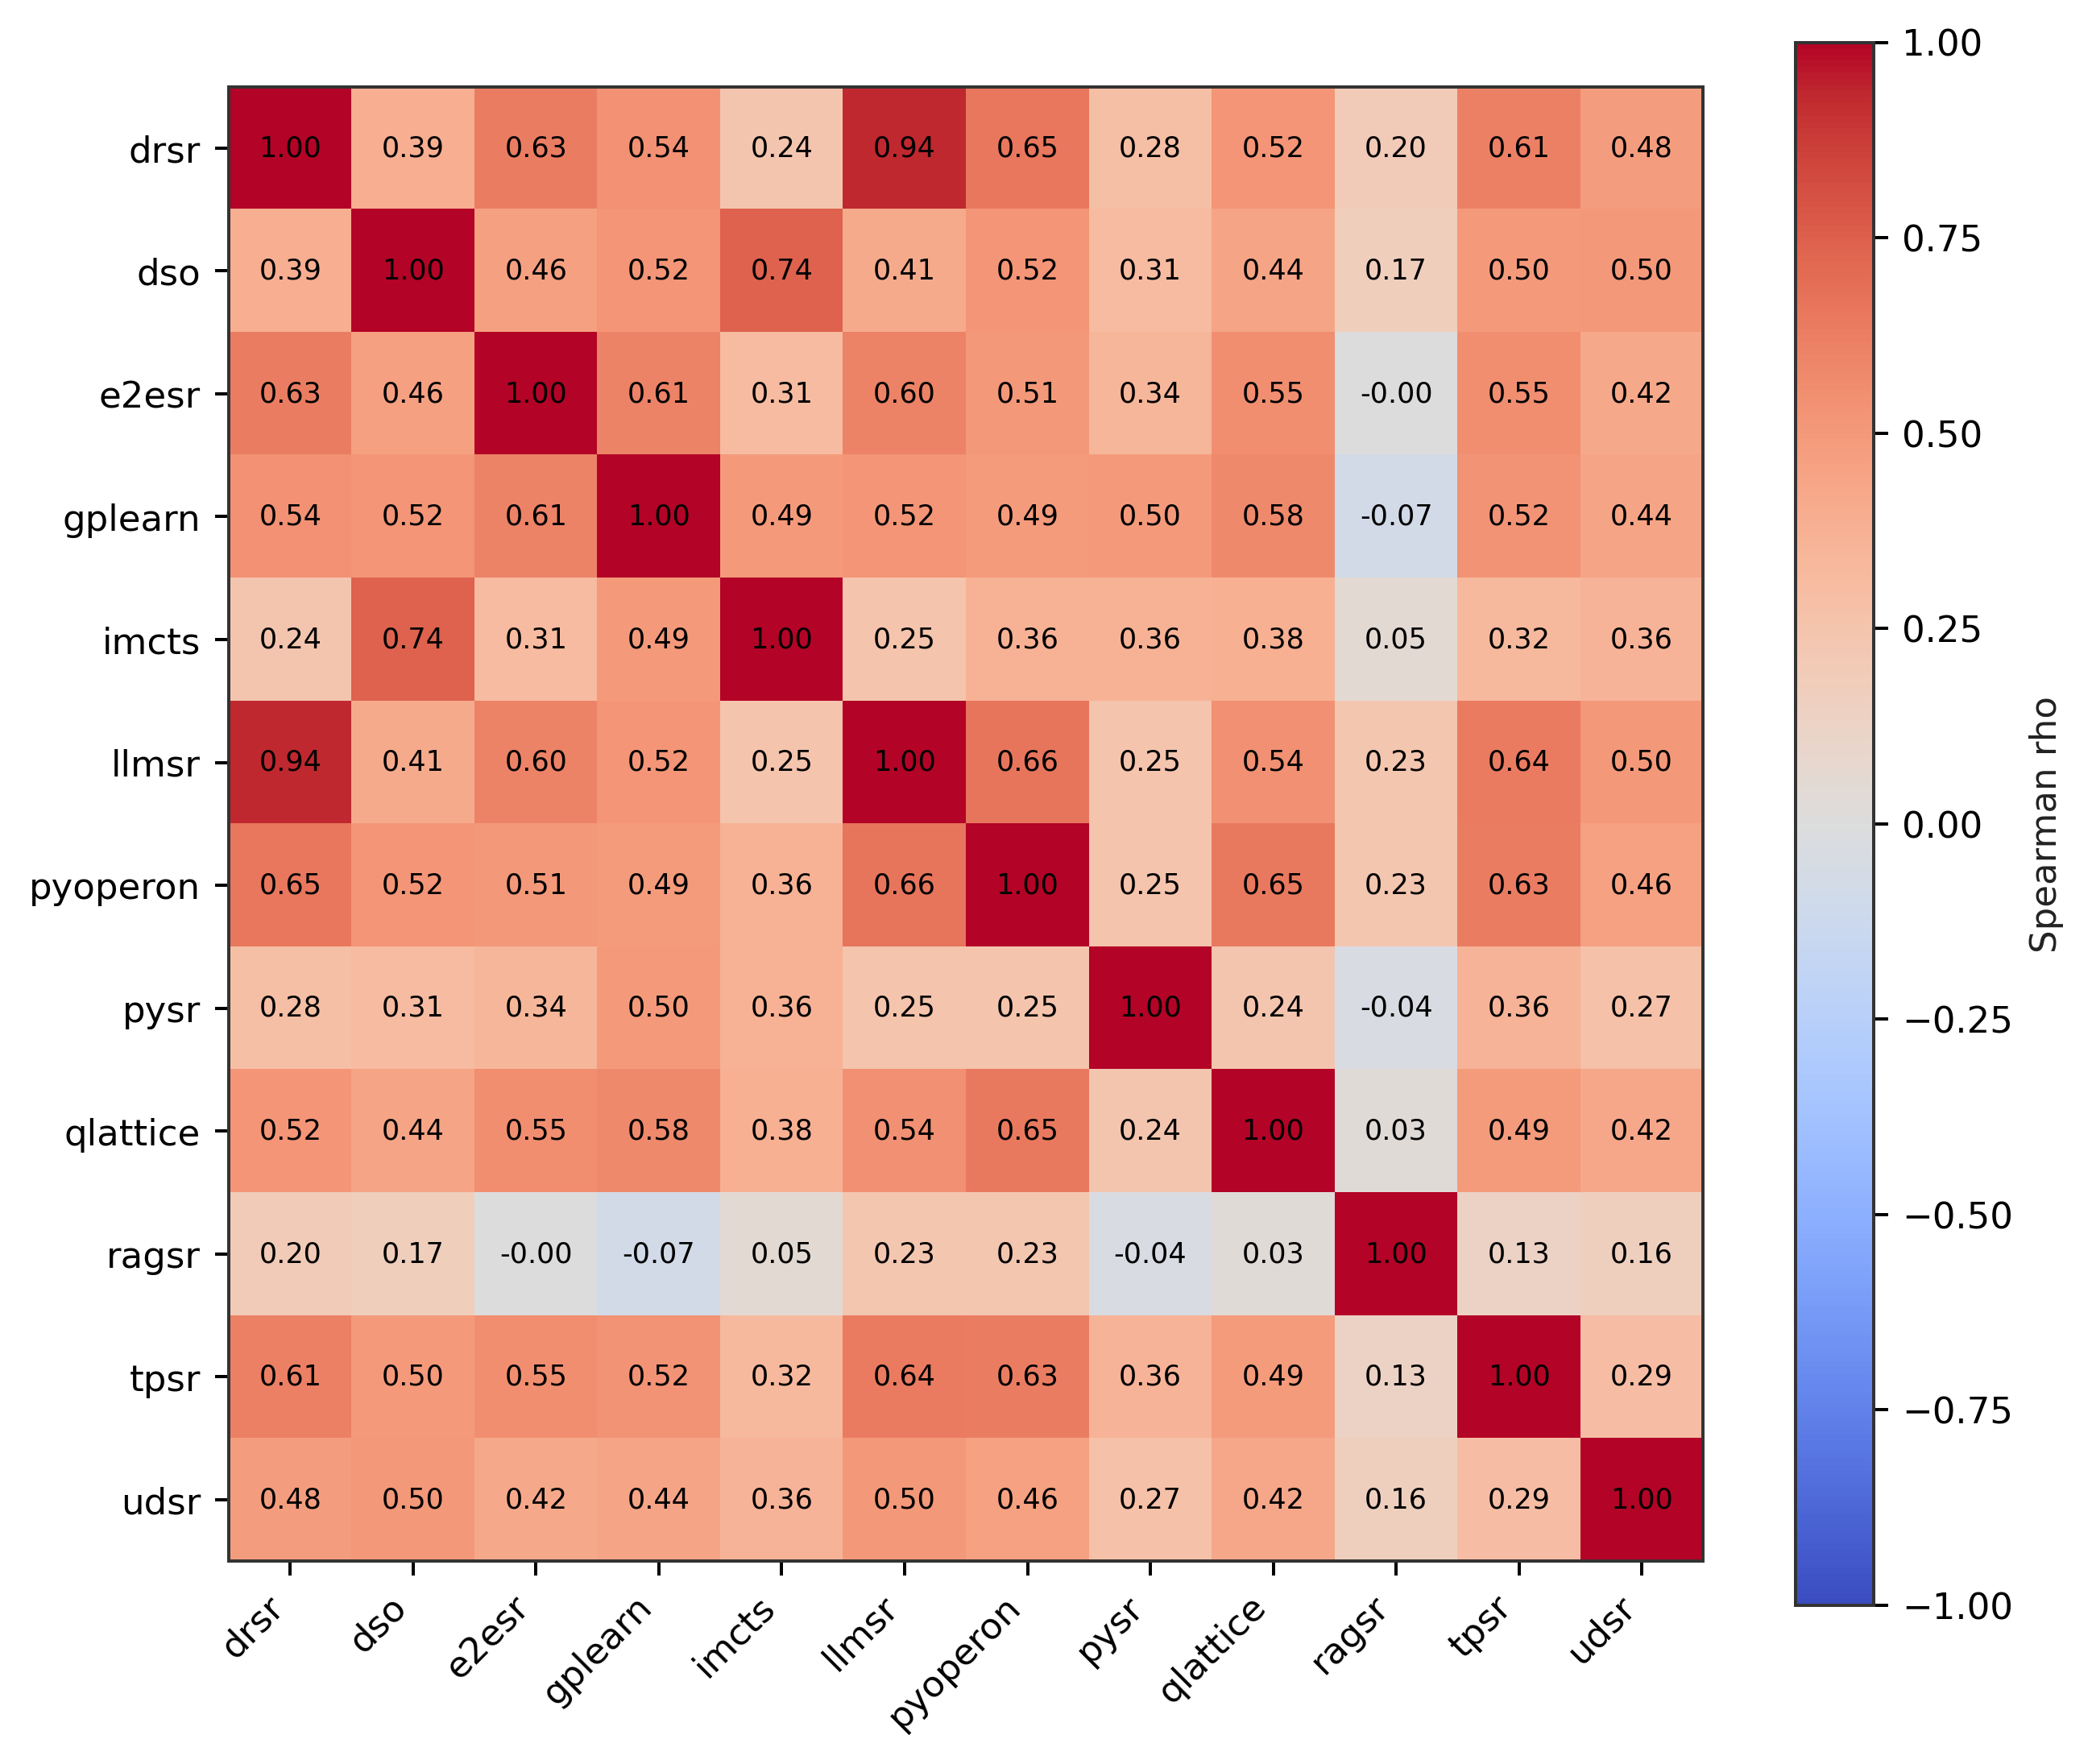
\includegraphics[width=0.68\linewidth]{imgs/Article/figure07_algorithm_behavior_correlation}
\caption{\textbf{Algorithm behavior correlation on Candidate-200.} The correlation structure is used to avoid selecting redundant probes.}
\label{fig:algorithm-behavior-correlation}
\end{figure}


\subsection{Probe4-Full Run Cleaning and Aggregation}
\label{app:probe4-run-cleaning}

The selected Probe-4 is evaluated on all 664 reservoir tasks with three seeds:
\[
664 \times 4 \times 3 = 7968.
\]
Each run records:
\[
\mathrm{dataset\_id},\ 
\mathrm{algorithm},\ 
\mathrm{seed},\ 
\mathrm{status},\ 
\mathrm{valid\_output},
\]
\[
e^{id},\ 
e^{ood},\ 
\mathrm{runtime},\ 
\mathrm{expression},\ 
\mathrm{complexity},\ 
\mathrm{failure\_reason}.
\]

Unfinished runs are not automatically treated as invalid runs. Each run first receives an outcome class:
\[
\{
\texttt{valid\_finite},
\texttt{valid\_extreme},
\texttt{partial},
\texttt{timeout\_no\_output},
\]
\[
\texttt{invalid},
\texttt{system\_error},
\texttt{not\_finished}
\}.
\]
Only finished runs with the correct dataset identity are evaluable. Valid extreme-error runs remain valid, and their NMSE values are clipped rather than dropped.

For every run, raw NMSE is mapped to clipped log space:
\[
\ell(x)
=
\mathrm{clip}
\left(
\log_{10}(\max(x,10^{-12})),
-12,
12
\right).
\]
For dataset \(i\), probe \(p\), and seed set \(\mathcal{S}\), the dataset--probe aggregates are:
\[
m_{i,p}^{id}
=
\mathrm{median}_{s\in\mathcal{S}_{valid}}
\ell(\mathrm{NMSE}_{i,p,s}^{id}),
\]
\[
m_{i,p}^{ood}
=
\mathrm{median}_{s\in\mathcal{S}_{valid}}
\ell(\mathrm{NMSE}_{i,p,s}^{ood}),
\]
\[
r_{i,p}
=
\frac{|\mathcal{S}_{valid}|}{|\mathcal{S}_{evaluable}|},
\]
\[
q_{i,p}^{id}
=
\mathrm{IQR}_{s\in\mathcal{S}_{valid}}
\ell(\mathrm{NMSE}_{i,p,s}^{id}),
\]
\[
q_{i,p}^{ood}
=
\mathrm{IQR}_{s\in\mathcal{S}_{valid}}
\ell(\mathrm{NMSE}_{i,p,s}^{ood}).
\]
If no valid seed is available for a dataset--probe pair, the pair is excluded from performance medians but contributes to invalid and timeout rates.


\subsection{Robust Normalization}
\label{app:robust-normalization}

All continuous selection features use robust min-max normalization:
\[
\mathrm{rmin}(x)=P_5(x),
\qquad
\mathrm{rmax}(x)=P_{95}(x),
\]
\[
\mathrm{Norm}(x)
=
\mathrm{clip}
\left(
\frac{x-\mathrm{rmin}(x)}
{\mathrm{rmax}(x)-\mathrm{rmin}(x)},
0,
1
\right).
\]
If \(\mathrm{rmax}(x)=\mathrm{rmin}(x)\), the normalized value is set to zero. Robust normalization prevents a small number of catastrophic NMSE explosions from dominating the selection score.


\subsection{Dataset-Level Information Score}
\label{app:dataset-information-score}

For each dataset \(i\), the Probe-4 response vector contains median ID/OOD quality, OOD-ID degradation, valid-output pattern, and seed variability. The discrimination score is
\[
\begin{aligned}
\mathrm{Disc}_i
={}&
0.35\,\mathrm{Norm}\!\left(\mathrm{Var}_{p}(m_{i,p}^{id})\right)
+
0.35\,\mathrm{Norm}\!\left(\mathrm{Var}_{p}(m_{i,p}^{ood})\right)\\
&+
0.15\,\mathrm{Norm}\!\left(\mathrm{Var}_{p}(m_{i,p}^{ood}-m_{i,p}^{id})\right)
+
0.10\,\mathrm{Norm}\!\left(\mathrm{Mean}_{p<q}|m_{i,p}^{ood}-m_{i,q}^{ood}|\right)\\
&+
0.05\,\mathrm{Norm}\!\left(H(\mathrm{valid\_pattern}_{i,:})\right).
\end{aligned}
\]
The instability score is
\[
\begin{aligned}
\mathrm{Instab}_i
={}&
0.40\,\mathrm{Mean}_{p}(q_{i,p}^{ood})
+
0.20\,\mathrm{Mean}_{p}(q_{i,p}^{id})
+
0.20\,\mathrm{Max}_{p}(q_{i,p}^{ood})\\
&+
0.10\,\mathrm{invalid\_rate}_i
+
0.10\,\mathrm{timeout\_rate}_i.
\end{aligned}
\]
The stability and information scores are
\[
\mathrm{Stab}_i
=
1-\mathrm{Norm}(\mathrm{Instab}_i),
\qquad
\mathrm{Info}_i
=
\mathrm{Disc}_i\cdot \mathrm{Stab}_i.
\]
Thus, a dataset receives high information only when it separates probes and the separation is not primarily caused by seed noise, invalid outputs, or timeout artifacts.


\subsection{Difficulty, Failure Mode, and Eligibility}
\label{app:difficulty-failure-eligibility}

Dataset difficulty is computed from the mean ID/OOD response across valid probes:
\[
\mathrm{Difficulty}_i
=
\mathrm{Mean}_{p}
\left[
\frac{
m_{i,p}^{id}
+
m_{i,p}^{ood}
}{2}
\right].
\]
Datasets are binned into easy, medium, hard, and extreme by robust quantiles. High invalid or timeout rates are allowed to override the bin to extreme.

Failure modes are assigned in priority order:
\[
\mathrm{incomplete},
\quad
\mathrm{invalid\mbox{-}prone},
\quad
\mathrm{one\mbox{-}sided},
\quad
\mathrm{unstable},
\]
\[
\mathrm{OOD\mbox{-}failure},
\quad
\mathrm{all\mbox{-}struggle},
\quad
\mathrm{one\mbox{-}method\mbox{-}wins},
\quad
\mathrm{all\mbox{-}good}.
\]
Eligibility is one of:
\[
\mathrm{eligible},
\quad
\mathrm{limited\mbox{-}quota},
\quad
\mathrm{excluded},
\quad
\mathrm{incomplete}.
\]
Limited-quota datasets are not discarded; they are allowed to enter \core{} only under explicit caps.


\subsection{Coverage and Balance Terms}
\label{app:coverage-balance}

For a categorical attribute \(a\), let \(\mathcal{C}_a(D)\) be the set of categories observed in the full reservoir and \(\mathcal{C}_a(S)\) those observed in a subset. Category coverage is
\[
\mathrm{Cov}_a(S)
=
\frac{
|\mathcal{C}_a(S)|
}{
|\mathcal{C}_a(D)|
}.
\]
Structural coverage averages coverage over family, subgroup, operator group, feature-count bin, sample-count bin, formula-complexity bin, OOD type, and dummy-variable status. Response coverage averages coverage over difficulty bin, failure mode, winner probe, and valid-output pattern:
\[
\mathrm{Coverage}(S)
=
0.6\,\mathrm{StructuralCoverage}(S)
+
0.4\,\mathrm{ResponseCoverage}(S).
\]

Balance measures distributional similarity to the full reservoir. For categorical attribute \(a\), let \(p_a^S\) and \(p_a^D\) be empirical distributions in the subset and the full reservoir. Total-variation similarity is
\[
\mathrm{Sim}_a(S,D)
=
1
-
\frac{1}{2}
\sum_c
|p_a^S(c)-p_a^D(c)|.
\]
The balance term is a weighted average of \(\mathrm{Sim}_a\) over structural and response-derived bins.


\subsection{Full Subset Objective and Hard Constraints}
\label{app:core50-objective-constraints}

The full subset score is
\[
J(S)
=
0.45\,\mathrm{Coverage}(S)
+
0.35\,\frac{1}{|S|}
\sum_{i\in S}\mathrm{Info}_i
+
0.20\,\mathrm{Balance}(S),
\]
subject to
\[
|S|=50.
\]
The objective is optimized only over feasible subsets. The main hard constraints are:
\begin{itemize}[leftmargin=*]
    \item semantic duplicate cap: each semantic duplicate group appears at most once;
    \item basename cap: no repeated basename in the released \core{} manifest;
    \item family quota: each family \(f\) receives a smoothed quota derived from reservoir frequency;
    \item subgroup concentration cap: no subgroup can dominate the selected subset;
    \item difficulty quota: easy, medium, hard, and extreme tasks must all be represented;
    \item limited-quota caps: invalid-prone, one-sided, unstable, and extreme cases are allowed but capped;
    \item materialization audit: result-derived columns are removed from the released manifest.
\end{itemize}

No source family receives a hand-written special rule. Let \(n_f\) be the number of reservoir tasks in family \(f\), and let \(F\) be the number of families. The smoothed target mass is
\[
t_f
=
0.6\frac{n_f}{664}
+
0.4\frac{1}{F}.
\]
The target count is
\[
q_f^{target}
=
50t_f,
\]
and the lower and upper quota bounds are
\[
q_f^{min}
=
\max(1,\lfloor q_f^{target}-1\rfloor),
\qquad
q_f^{max}
=
\lceil q_f^{target}+2\rceil.
\]
This allocation gives larger families more capacity, prevents smaller families from disappearing, and avoids domination by any single source family.

The realized \core{} family counts are:
\[
16\ \mathrm{LLM\mbox{-}SRBench},
\quad
15\ \mathrm{SRSD},
\quad
9\ \mathrm{SRBench1.0},
\]
\[
3\ \mathrm{Nguyen},
\quad
2\ \mathrm{SRBench2025},
\quad
2\ \mathrm{Korns},
\quad
2\ \mathrm{Keijzer},
\quad
1\ \mathrm{Vladislavleva}.
\]
Each selected basename appears once.


\subsection{Search Procedure}
\label{app:core50-search}

Selection is implemented as constrained local search:
\begin{enumerate}[leftmargin=*]
    \item construct an initial feasible subset using family quotas and high-information eligible datasets;
    \item repair hard-constraint violations, especially duplicates and over-concentrated subgroups;
    \item evaluate \(J(S)\) for the feasible subset;
    \item repeatedly propose one-for-one swaps that preserve feasibility;
    \item accept swaps that improve \(J(S)\);
    \item run multiple random restarts and retain the highest-scoring feasible subset;
    \item export the frozen manifest and a selection audit report.
\end{enumerate}

This procedure is deliberately auditable rather than opaque. The released artifact records the input dataset-level table, selection scores, selected manifest, and post-selection balance report.


\subsection{Baseline Subset Definitions}
\label{app:baseline-selectors}

\core{} is compared with several 50-task alternatives:
\begin{itemize}[leftmargin=*]
    \item \textbf{random-50}: uniformly sampled 50-task subsets;
    \item \textbf{family-stratified random-50}: random subsets sampled approximately proportional to family sizes;
    \item \textbf{top-info-50}: top 50 datasets by \(\mathrm{Info}_i\);
    \item \textbf{metadata-diverse-50}: metadata-only diverse subset using feature count, formula complexity, sample count, and family coverage;
    \item \textbf{response-medoids-50}: response-space medoids in the four-probe ID/OOD/validity/stability feature space;
    \item \textbf{difficulty-balanced-50}: quota-balanced subset over difficulty bins, with high-information tie-breaks.
\end{itemize}


\subsection{Validation Diagnostics}
\label{app:core50-validation-diagnostics}

The validation compares \core{} and alternative 50-task selectors using:
\[
\mathrm{Coverage},
\quad
\mathrm{MeanInfo},
\quad
\mathrm{RankFidelity},
\quad
\mathrm{Stability},
\quad
\mathrm{NonRedundancy},
\quad
\mathrm{DifficultyBalance}.
\]
These columns are diagnostic criteria rather than independent optimization targets. \core{} is selected for their constrained trade-off together with hard feasibility constraints.

\begin{table}[ht]
\centering
\small
\caption{\textbf{Subset-quality summary for \core{} and alternative 50-task selectors.} Higher is better within each diagnostic column, but \core{} is selected for a constrained trade-off rather than for optimizing any single column.}
\label{tab:core50-baseline-quality-audit}
\resizebox{\linewidth}{!}{%
\begin{tabular}{lrrrrrr}
\toprule
Subset & Coverage & Mean info & Rank fidelity & Stability & Non-red. & Diff. balance \\
\midrule
\core{} & 0.838 & 0.471 & 1.000 & 0.835 & 0.769 & 0.892 \\
top-info-50 & 0.784 & 0.691 & 1.000 & 0.911 & 0.860 & 0.780 \\
metadata-diverse-50 & 0.635 & 0.085 & 1.000 & 0.735 & 0.860 & 0.601 \\
difficulty-balanced-50 & 0.817 & 0.637 & 1.000 & 0.883 & 0.920 & 0.999 \\
random-50 avg & 0.835 & 0.187 & 0.983 & 0.705 & 0.970 & 0.908 \\
family-stratified random-50 avg & 0.815 & 0.191 & 0.995 & 0.696 & 0.968 & 0.909 \\
\bottomrule
\end{tabular}
}
\end{table}

\subsection{Release and Leakage Control}
\label{app:core50-release-leakage}

After validation, \core{} is frozen as the official benchmark subset. Probe4-Full results are used only for benchmark construction. The final leaderboard is recomputed independently by running all 12 algorithms on frozen \core{} with five seeds:$12\times 50\times 5 = 3000.$

The released \core{} manifest contains dataset identity and static metadata needed for benchmark materialization. It excludes result-derived columns such as probe gap, priority score, selected advantage side, Probe-4 informativeness score, and selection rank. This prevents downstream methods from directly exploiting construction signals.

The frozen benchmark release includes:
\[
\mathrm{core50\_v1.json},
\qquad
\mathrm{core50\_metadata.csv},
\qquad
\mathrm{core50\_selection\_report.pdf}.
\]

\Cref{tab:core50-ablation-summary} reports the subset-quality summary used for the main-text validation table. The composite objective summarizes the coverage--information--stability trade-off, while aggregate-score MAE measures fidelity to the full 664-task reservoir. The important empirical pattern is that single-axis selectors can improve one summary dimension, but they lose substantially more full-reservoir fidelity than \core{}.

\begin{table}[t]
\centering
\small
\caption{\textbf{Core-50 ablation against deterministic and random 50-task selectors.} Higher is better for objective score, coverage, mean information, and mean stability; lower is better for aggregate-score MAE.}
\label{tab:core50-ablation-summary}
\resizebox{\linewidth}{!}{%
\begin{tabular}{lrrrrr}
\toprule
\textbf{Selector} & \textbf{Objective} & \textbf{Coverage} & \textbf{Mean info} & \textbf{Mean stability} & \textbf{Agg. MAE} \\
\midrule
Random avg & 0.6157 & \textbf{0.7804} & 0.1949 & 0.7070 & 0.4949 \\
Family-random avg & 0.6105 & 0.7772 & 0.1910 & 0.6912 & 0.5243 \\
Metadata-diverse & 0.6744 & 0.7712 & 0.3738 & 0.8340 & 0.5060 \\
Response-space K-medoids & 0.6342 & 0.7660 & 0.2726 & 0.6258 & 0.6044 \\
Top-information & \textbf{0.7305} & 0.7216 & \textbf{0.6049} & 0.8931 & 1.0339 \\
Difficulty-balanced & 0.6957 & 0.7122 & 0.5145 & 0.8375 & 1.0430 \\
\core{} & 0.7284 & 0.7736 & 0.5308 & \textbf{0.8997} & \textbf{0.1388} \\
\bottomrule
\end{tabular}
}
\end{table}



\clearpage
\setcounter{figure}{0}
\renewcommand{\thefigure}{C.\arabic{figure}}
\renewcommand{\theHfigure}{appendixC.\arabic{figure}}
\section{Infrastructure and Data-Cleaning Details}
\label{app:infra-cleaning}

This appendix documents the engineering substrate used to produce the reported benchmark results. The goal is not to prescribe one implementation stack, but to make clear which parts of \arena{} are part of the benchmark contract and which parts are deployment choices. We describe the implementation paths that matter for reproducibility: how a run is launched, how wrappers are constrained, how intermediate results are recovered, and how the dataset pool is cleaned before benchmark distillation.

\subsection{Layered execution architecture}

\arena{} separates algorithm integration from benchmark execution through four layers.

\begin{center}
\small
\begin{tabular}{p{0.20\linewidth}p{0.31\linewidth}p{0.39\linewidth}}
\toprule
\textbf{Layer} & \textbf{Main artifact} & \textbf{Responsibility} \\
\midrule
Configuration & \texttt{toolbox\_config.json}, \texttt{envs\_config.json} & Map each tool to a wrapper class and environment \\
Front-end API & \texttt{SymbolicRegressor} & Expose \texttt{fit}, \texttt{predict}, equation extraction, and artifact export \\
Isolation runner & \texttt{subprocess\_runner.py} & Execute wrapper commands in the configured environment \\
Benchmark runner & \texttt{benchmarks/runner.py} & Load data, inject contracts, evaluate metrics, and write artifacts \\
\bottomrule
\end{tabular}
\end{center}

The benchmark never calls an upstream algorithm repository directly. Instead, a run is issued as a JSON command containing the action, data array, seed, budget, and framework parameters. The subprocess runner imports the appropriate wrapper module, executes the action, serializes the fitted wrapper state, and returns a JSON response. This design lets the benchmark keep a stable interface even when the underlying algorithms expose incompatible APIs.

\subsection{Wrapper contract}

Each algorithm wrapper implements a minimal estimator interface:
\begin{verbatim}
fit(X, y)
predict(X)
get_optimal_equation()
get_total_equations()
export_canonical_symbolic_program()
\end{verbatim}
The first four methods are the execution interface. The last method is the symbolic-artifact interface: it exports a \texttt{CanonicalSymbolicProgram} containing the raw equation, normalized expression, variables, fitted constants when available, operator set, AST size, tree depth, and validation notes. When a wrapper cannot directly provide a complete canonical artifact, the result layer applies tool-specific normalizers to translate outputs such as PySR expressions, gplearn prefix trees, DSO/uDSR expressions, PyOperon strings, TPSR/E2ESR candidates, iMCTS outputs, and LLM-generated Python functions into the shared representation.

The benchmark runner also injects an explicit data contract into every wrapper:
\begin{verbatim}
n_features
feature_names
target_name
seed
timeout_in_seconds
exp_path
exp_name
\end{verbatim}
Wrappers validate that the declared feature count and names match the actual training matrix. This avoids a common SR-integration failure mode: a method silently using the wrong number of input variables or emitting an out-of-range variable token. For LLM-based methods, \arena{} separates the real data contract from the prompt contract. The runner can expose canonical prompt variables while preserving original feature names, target names, metadata-derived background, and optional anonymization switches.

\subsection{Environment isolation and why Docker is not the primary boundary}

\arena{} uses per-tool conda environments plus subprocess isolation as the canonical evaluation boundary. The current 12-method panel requires incompatible Python and package stacks: for example, the base GP/PySR/PyOperon environment uses Python 3.10, DSO/uDSR and E2ESR use Python 3.7, TPSR uses Python 3.9, and LLM-backed methods use a separate LLM environment. Some methods also require external assets such as pretrained weights, Julia/PySR caches, GPU libraries, or API-backed LLM configuration.

Docker is useful for lightweight demonstration and single-environment deployment, but it is not used as the primary benchmark boundary for three practical reasons. First, a single container that includes all 12 algorithms would be large, slow to rebuild, and brittle because it would have to mix mutually incompatible Python and native dependencies. Second, the reported experiments run on heterogeneous CPU/GPU cluster nodes where user-level conda environments, mounted datasets, local model weights, Julia caches, and private LLM configuration files are easier to manage than privileged container builds. Third, the benchmark requires fine-grained process supervision: per-run timeout recovery, stdout/stderr forwarding, result-file recovery, and minute-level progress extraction are naturally handled by the subprocess runner. The artifact therefore records environment specifications and wrapper versions, while Docker remains an optional packaging layer rather than the source of evaluation semantics.

\subsection{Result, timeout, and progress semantics}

Every run writes a canonical \texttt{result.json} containing the tool name, dataset identity, seed, sanitized parameters, status, termination reason, final expression, canonical symbolic artifact, train/validation/ID/OOD metrics, runtime, and experiment directory. Sensitive keys such as API keys or tokens are removed from saved parameter dictionaries.

\arena{} distinguishes engineering failure from algorithmic failure. A run can be:
\begin{itemize}[leftmargin=*]
    \item \texttt{ok}: completed or budget-exhausted with a recovered, evaluable best-so-far expression;
    \item \texttt{timed\_out}: budget exhausted without a recoverable evaluable expression;
    \item \texttt{no\_valid\_output}: the method ran but produced no expression that can be evaluated on the required splits;
    \item \texttt{error}: wrapper, environment, data-loading, or execution error.
\end{itemize}
For snapshot-capable tools, the runner polls the algorithm's current-best state every 60 seconds and writes a minute-level JSON file under \texttt{progress/}. If the final expression is numerically unstable or a timeout occurs, the runner can recover the latest evaluable snapshot and mark the run as budget-exhausted with output instead of discarding the run.

\subsection{Dataset sources and acquisition}

The dataset repository is maintained separately from the paper source and the algorithm code. In the released artifact, datasets are accessed through stable manifest entries rather than copied into the experiment directory. Each manifest row stores the dataset identity, source family, subgroup, relative data path, split files, metadata file, and ground-truth formula file when available. This keeps the benchmark reproducible while avoiding multiple drifting copies of the same raw data.

The canonical data root is organized as
\begin{verbatim}
sim-datasets-data/<family>/<subgroup>/<dataset>/
\end{verbatim}
or, for compact classical families,
\begin{verbatim}
sim-datasets-data/<family>/<dataset>/
\end{verbatim}
The same layout is used locally, on the compute cluster, and in the public dataset package. The dataset package can be obtained either as a Git-LFS backed repository from Hugging Face or ModelScope, or through the lightweight \texttt{sim-datasets} Python package. During cluster execution, run manifests resolve paths such as \texttt{sim-datasets-data/...} against the configured dataset root, not against a partial checkout inside the code repository.

\begin{center}
\small
\begin{tabular}{p{0.22\linewidth}p{0.28\linewidth}p{0.40\linewidth}}
\toprule
\textbf{Source family} & \textbf{Role in the reservoir} & \textbf{Normalization notes} \\
\midrule
SRSD & Formula-backed scientific discovery tasks with Feynman-style equations and dummy-variable variants & Preserve SRSD subgroup labels, dummy-variable status, source citations, and \texttt{formula.py}; normalize Feynman identifiers for duplicate detection \\
LLM-SRBench & Physics, chemistry, materials, biological growth, and transformed equation-discovery tasks & Preserve semantic feature/target descriptions for prompt-controlled LLM evaluation while also supporting anonymized-variable runs \\
SRBench 1.0 & Feynman and Strogatz-style benchmark tasks used in prior SR evaluation & Convert source naming into the shared family/subgroup/basename scheme and audit cross-source Feynman duplicates \\
SRBench2025 first-principles & Compact first-principles tasks with small sample counts and explicit scientific formulas & Preserve original descriptions, units when available, and source-derived or table-derived OOD splits \\
Nguyen, Keijzer, Korns, Vladislavleva & Classical synthetic SR families used as controlled baselines & Generate deterministic train/validation/ID/OOD splits from formula specifications and record the generation rule in metadata \\
\bottomrule
\end{tabular}
\end{center}

The resulting \reservoir{} is therefore not a single upstream benchmark. It is a normalized union of formula-backed tasks from SRSD, LLM-SRBench, SRBench 1.0, SRBench2025 first-principles tasks, and classical synthetic families. Source family and subgroup are retained as first-class metadata fields so later selection stages can control coverage rather than treating the reservoir as an anonymous pool.

\subsection{Dataset format and validation}

All datasets are normalized into one executable directory format:
\begin{verbatim}
train.csv
valid.csv
id_test.csv
ood_test.csv        # optional but required for OOD analysis
metadata.yaml
formula.py          # required for ground-truth reservoir tasks
\end{verbatim}
The CSV files contain only numeric columns. The target column is not inferred from position during evaluation; it is read from \texttt{metadata.yaml}. The ordered feature list in metadata is the authoritative input signature and must match the non-target CSV columns. This matters for SR because variable order is part of the equation semantics: a valid expression over the wrong feature ordering is treated as an integration error rather than an algorithmic result.

The metadata records dataset name, source family, subgroup, split files and sample counts, ordered feature names, target name, feature and target descriptions when available, train/OOD ranges, license/source information, upstream resources, and the ground-truth formula file. When a source benchmark provides physical or semantic feature descriptions, \arena{} preserves them in metadata. LLM-based methods can then be evaluated either with semantic background enabled or with anonymized variables, while non-LLM methods receive the same numeric arrays and data contract.

Split construction follows a deterministic policy. If the upstream source already provides train, validation, ID-test, or OOD-test splits, those splits are preserved after header and type normalization. If a source provides only a single formula-backed table, \arena{} uses a fixed random seed to produce train/validation/ID splits and, when a reliable formula and feature domain are available, synthesizes an OOD split by sampling outside the training support and replaying the ground-truth formula. If no reliable OOD definition is available, the pipeline does not fabricate an OOD split; the gap is recorded in metadata and the dataset is excluded from OOD-dependent analyses.

For ground-truth tasks, \texttt{formula.py} is part of the benchmark contract. It exposes a deterministic callable evaluated using the metadata feature order. The validation script checks that required splits exist, files are not Git-LFS pointer stubs, CSV headers agree across splits, target columns exist, declared sample counts match row counts, all feature and target columns are numeric, \texttt{metadata.yaml} agrees with the CSV schema, and \texttt{formula.py} reproduces split targets within numeric tolerance. It also verifies that formula replay produces finite values on the declared OOD split; otherwise the dataset is marked for repair or manual review before it can enter reservoir selection.

\subsection{Cleaning and audit pipeline}

The data-cleaning pipeline is deliberately split into mechanical repairs and human-review gaps. Mechanically derivable fields are filled only when they can be computed from local files: missing \texttt{ground\_truth\_formula.file} is filled when \texttt{formula.py} exists, split ratios are computed from sample counts, formula NMSE is computed by replaying \texttt{formula.py} on split CSVs, and target OOD ranges are computed from \texttt{ood\_test.csv}. Fields requiring semantic judgment, such as citation text or feature descriptions for black-box variables, are not hallucinated; they are emitted into a manual-gap report.

\arena{} also audits common dataset-packaging failures before selection. Git-LFS pointer files are detected before interpreting CSV headers. All selected manifests are resolved against the real dataset root rather than a partial repository mirror. Dataset identity fields are normalized so that local paths, remote paths, and \texttt{sim-datasets-data/...} relative paths map to the same identity. This prevents false missing-file reports and avoids accidentally evaluating a result on the wrong dataset.

\subsection{Semantic duplicate removal and final materialization}

Before constructing the final benchmark, \arena{} performs semantic duplicate detection on the internal 100-task clean pool used during development. For Feynman-style tasks, names are normalized into a canonical Feynman identifier. For general formula-backed tasks, \texttt{formula.py} is parsed, function arguments are normalized to \texttt{x0}, \texttt{x1}, \ldots, and a symbolic expression hash is computed from the simplified expression tree. If multiple tasks share a semantic key, the pipeline retains the highest-priority representative and fills the removed slot from \textsc{Candidate-200} using nearest-neighbor replacement under family, subgroup, selection-mode, advantage-side, feature-count, sample-count, and formula-complexity similarity.

The final materialization step intentionally excludes result-derived columns such as priority score, probe gap, quality score, stability score, selected advantage side, and selection mode. It uses only static attributes: family, subgroup, dummy-variable flag, feature count, sample scale, and formula complexity. A randomized search and audit report family/subgroup balance and static numeric summaries. Finally, selected datasets are materialized through manifest files and stable links, so the benchmark is auditable without duplicating raw data directories.


\clearpage
\setcounter{figure}{0}
\renewcommand{\thefigure}{D.\arabic{figure}}
\renewcommand{\theHfigure}{appendixC1.\arabic{figure}}
\section{Reservoir Construction Details}
\label{app:reservoir}

\subsection{Ground-truth filtering criteria}

The initial candidate pool contains more than 800 symbolic regression tasks collected from heterogeneous benchmark families and equation-discovery sources. A task is retained in the ground-truth reservoir only if it satisfies the following evaluation-readiness criteria:
\begin{itemize}
    \item a ground-truth formula is available;
    \item the formula is parsable into a symbolic expression tree;
    \item all variables, constants, and operators are resolvable;
    \item the expression can be executed as a numerical program;
    \item fixed train, ID test, and OOD test splits are available or can be deterministically generated;
    \item target values are finite on all official splits;
    \item the expression variable signature matches the dataset columns;
    \item metadata is sufficient for provenance, structural auditing, and duplicate control.
\end{itemize}

Tasks are removed if they have missing or ambiguous ground-truth formulas, unparsable expressions, unresolved variables, invalid operators, non-finite targets, inconsistent stored targets, missing official splits, or insufficient metadata. After filtering, the ground-truth reservoir contains $|D_{\mathrm{GT}}| = 664$ tasks.

\subsection{Reservoir composition}

After applying the ground-truth filtering criteria, the retained tasks are audited to verify that the reservoir has not collapsed into a narrow subset of formulas or source families. This audit summarizes the 664-task \reservoir{} from both provenance and structural perspectives, including source family, operator usage, formula complexity, and probe-derived difficulty bins.

\begin{figure}[p]
\centering
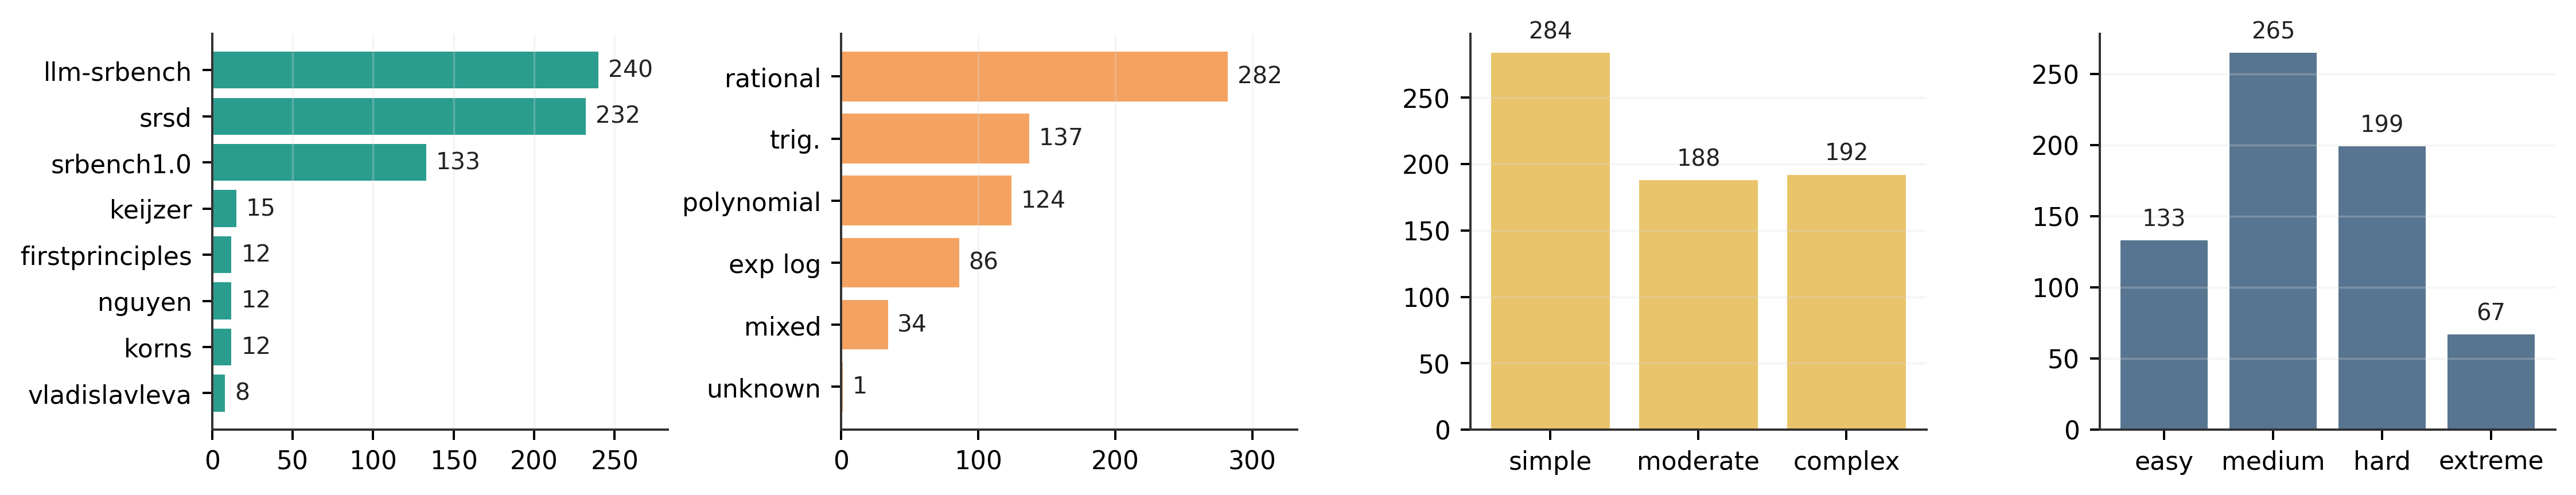
\includegraphics[width=0.88\linewidth]{imgs/Article/figure02_reservoir_composition}
\caption{\textbf{\reservoir{} composition after ground-truth filtering.} The 664-task reservoir retains heterogeneous source families, operator profiles, formula complexities, and probe-derived difficulty bins.}
\label{fig:appendix-reservoir-composition}
\end{figure}

As shown in \cref{fig:appendix-reservoir-composition}, the filtered reservoir remains heterogeneous across dataset provenance, symbolic structure, and empirical difficulty. These composition statistics are used to document the parent task population represented by \core{}, while the actual core-set selection procedure is described separately in the main text.


\subsection{Unified task schema}

Each retained task is stored with a unified schema. The core fields are summarized in \cref{tab:reservoir-schema}.

\begin{table}[t]
\centering
\caption{\textbf{Core fields stored for each task in the ground-truth reservoir.}}
\label{tab:reservoir-schema}
\begin{tabular}{ll}
\toprule
Field & Description \\
\midrule
\texttt{dataset\_id} & Unique task identifier \\
\texttt{family} & Source family or benchmark family \\
\texttt{subgroup} & Sub-family, variant, or task group \\
\texttt{basename} & Original equation or task name \\
\texttt{source\_benchmark} & Original source benchmark \\
\texttt{ground\_truth\_formula} & Raw ground-truth expression \\
\texttt{canonical\_formula} & Canonicalized expression \\
\texttt{train\_split} & Training samples \\
\texttt{id\_test\_split} & In-distribution test samples \\
\texttt{ood\_test\_split} & Out-of-distribution test samples \\
\texttt{n\_features} & Number of input variables \\
\texttt{sample\_count} & Number of samples in each split \\
\texttt{formula\_complexity} & Expression complexity score \\
\texttt{operator\_types} & Operators appearing in the formula \\
\texttt{ood\_type} & Type of OOD split \\
\texttt{dummy\_variable\_flag} & Whether dummy variables are present \\
\texttt{semantic\_duplicate\_group} & Duplicate-control group identifier \\
\bottomrule
\end{tabular}
\end{table}

\subsection{Expression canonicalization}

All ground-truth formulas are converted into a unified symbolic representation. The canonicalization procedure standardizes variable names, operator names, constant formatting, commutative ordering, and expression-tree serialization. For each formula, the following representations are stored:
\begin{itemize}
    \item canonical expression string;
    \item prefix and postfix forms;
    \item expression tree;
    \item operator-normalized form;
    \item constant-normalized form;
    \item Newick-like tree serialization;
    \item canonical skeleton for duplicate and structural-consistency analysis.
\end{itemize}

The raw source expression is also retained to preserve provenance. The canonical representation is used for symbolic equivalence testing, expression-tree comparison, operator and variable recovery, duplicate detection, and seed-level structural consistency in the leaderboard evaluation.

\subsection{Train, ID, and OOD splits}

Each retained task contains fixed train, ID test, and OOD test splits. The training split is used by algorithms during expression search. The ID test split evaluates same-distribution generalization, while the OOD test split evaluates whether the discovered expression extrapolates beyond the training distribution.

If a source benchmark provides compatible official splits, those splits are preserved. Otherwise, splits are deterministically generated from the executable ground-truth program and recorded in the task metadata. Official numerical scores are computed only on the fixed ID and OOD test splits.

\subsection{Quality-control checks}

The following checks are applied before a task enters the reservoir:
\begin{itemize}
    \item expression parsing succeeds;
    \item executable ground-truth program produces finite values on all official splits;
    \item stored targets match executable ground-truth outputs within numerical tolerance;
    \item variable signatures match dataset columns;
    \item canonicalization is deterministic;
    \item required metadata fields are present;
    \item duplicate identifiers and ambiguous records are resolved.
\end{itemize}

These checks ensure that the 664-task reservoir is not merely a collection of regression tables, but a standardized and executable substrate for numerical evaluation, symbolic comparison, and later leaderboard analysis.


\clearpage
\setcounter{figure}{0}
\renewcommand{\thefigure}{D.\arabic{figure}}
\renewcommand{\theHfigure}{appendixD.\arabic{figure}}
\section{Additional Empirical Figures}
\label{app:additional-figures}

The main text keeps only the figures needed for the core narrative. This appendix retains supporting diagnostics that are useful for auditability but would distract from the main flow.

% \begin{figure}[p]
% \centering
% 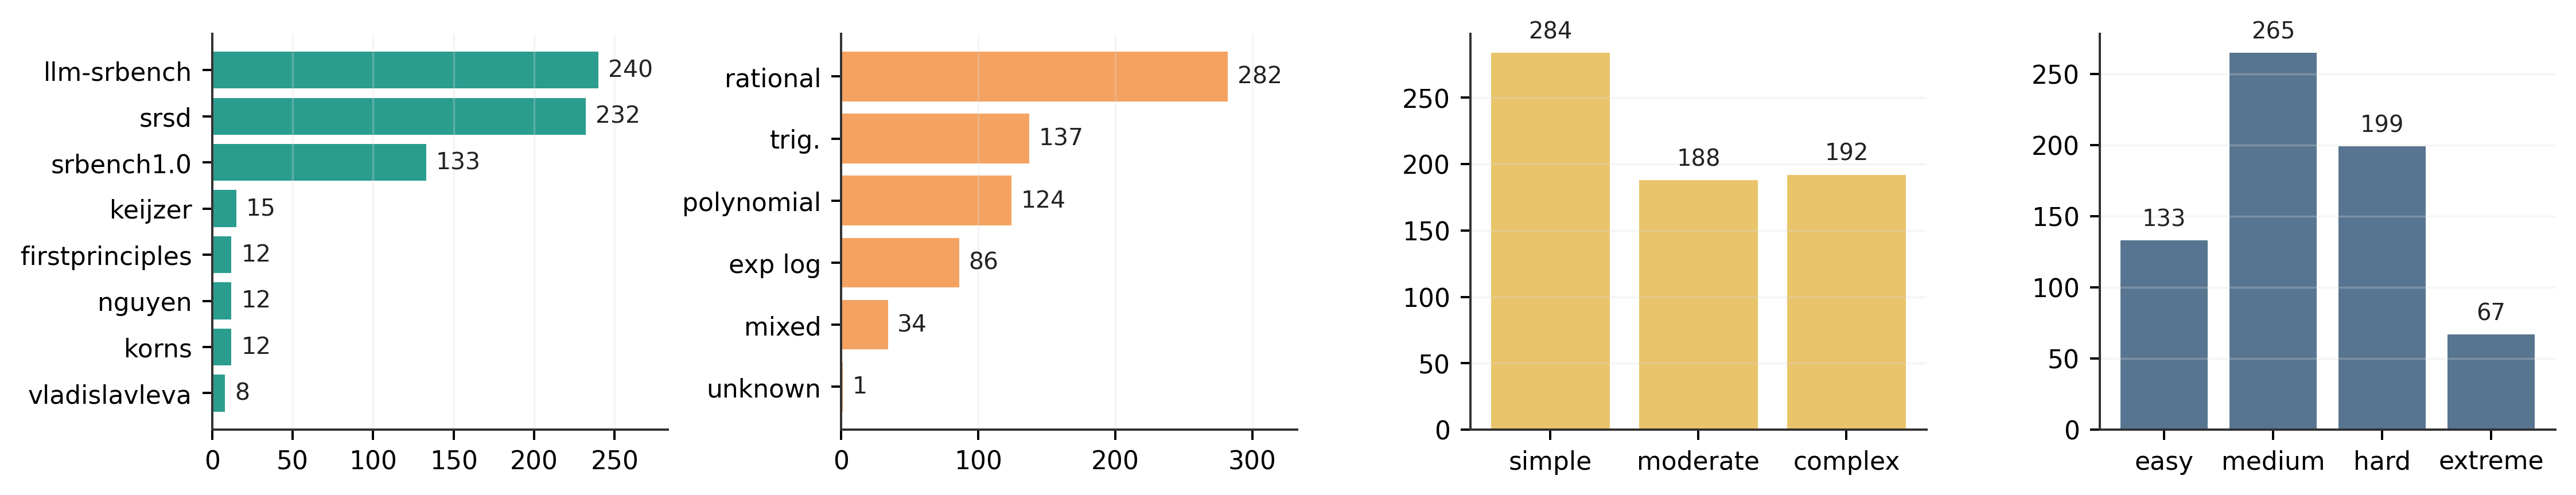
\includegraphics[width=0.88\linewidth]{imgs/Article/figure02_reservoir_composition}
% \caption{\reservoir{} composition after ground-truth filtering. The reservoir retains heterogeneous source families, operator profiles, formula complexities, and probe-derived difficulty bins; this is why later selection must control both static metadata and response-derived behavior.}
% \label{fig:appendix-reservoir-composition}
% \end{figure}

\begin{figure}[p]
\centering
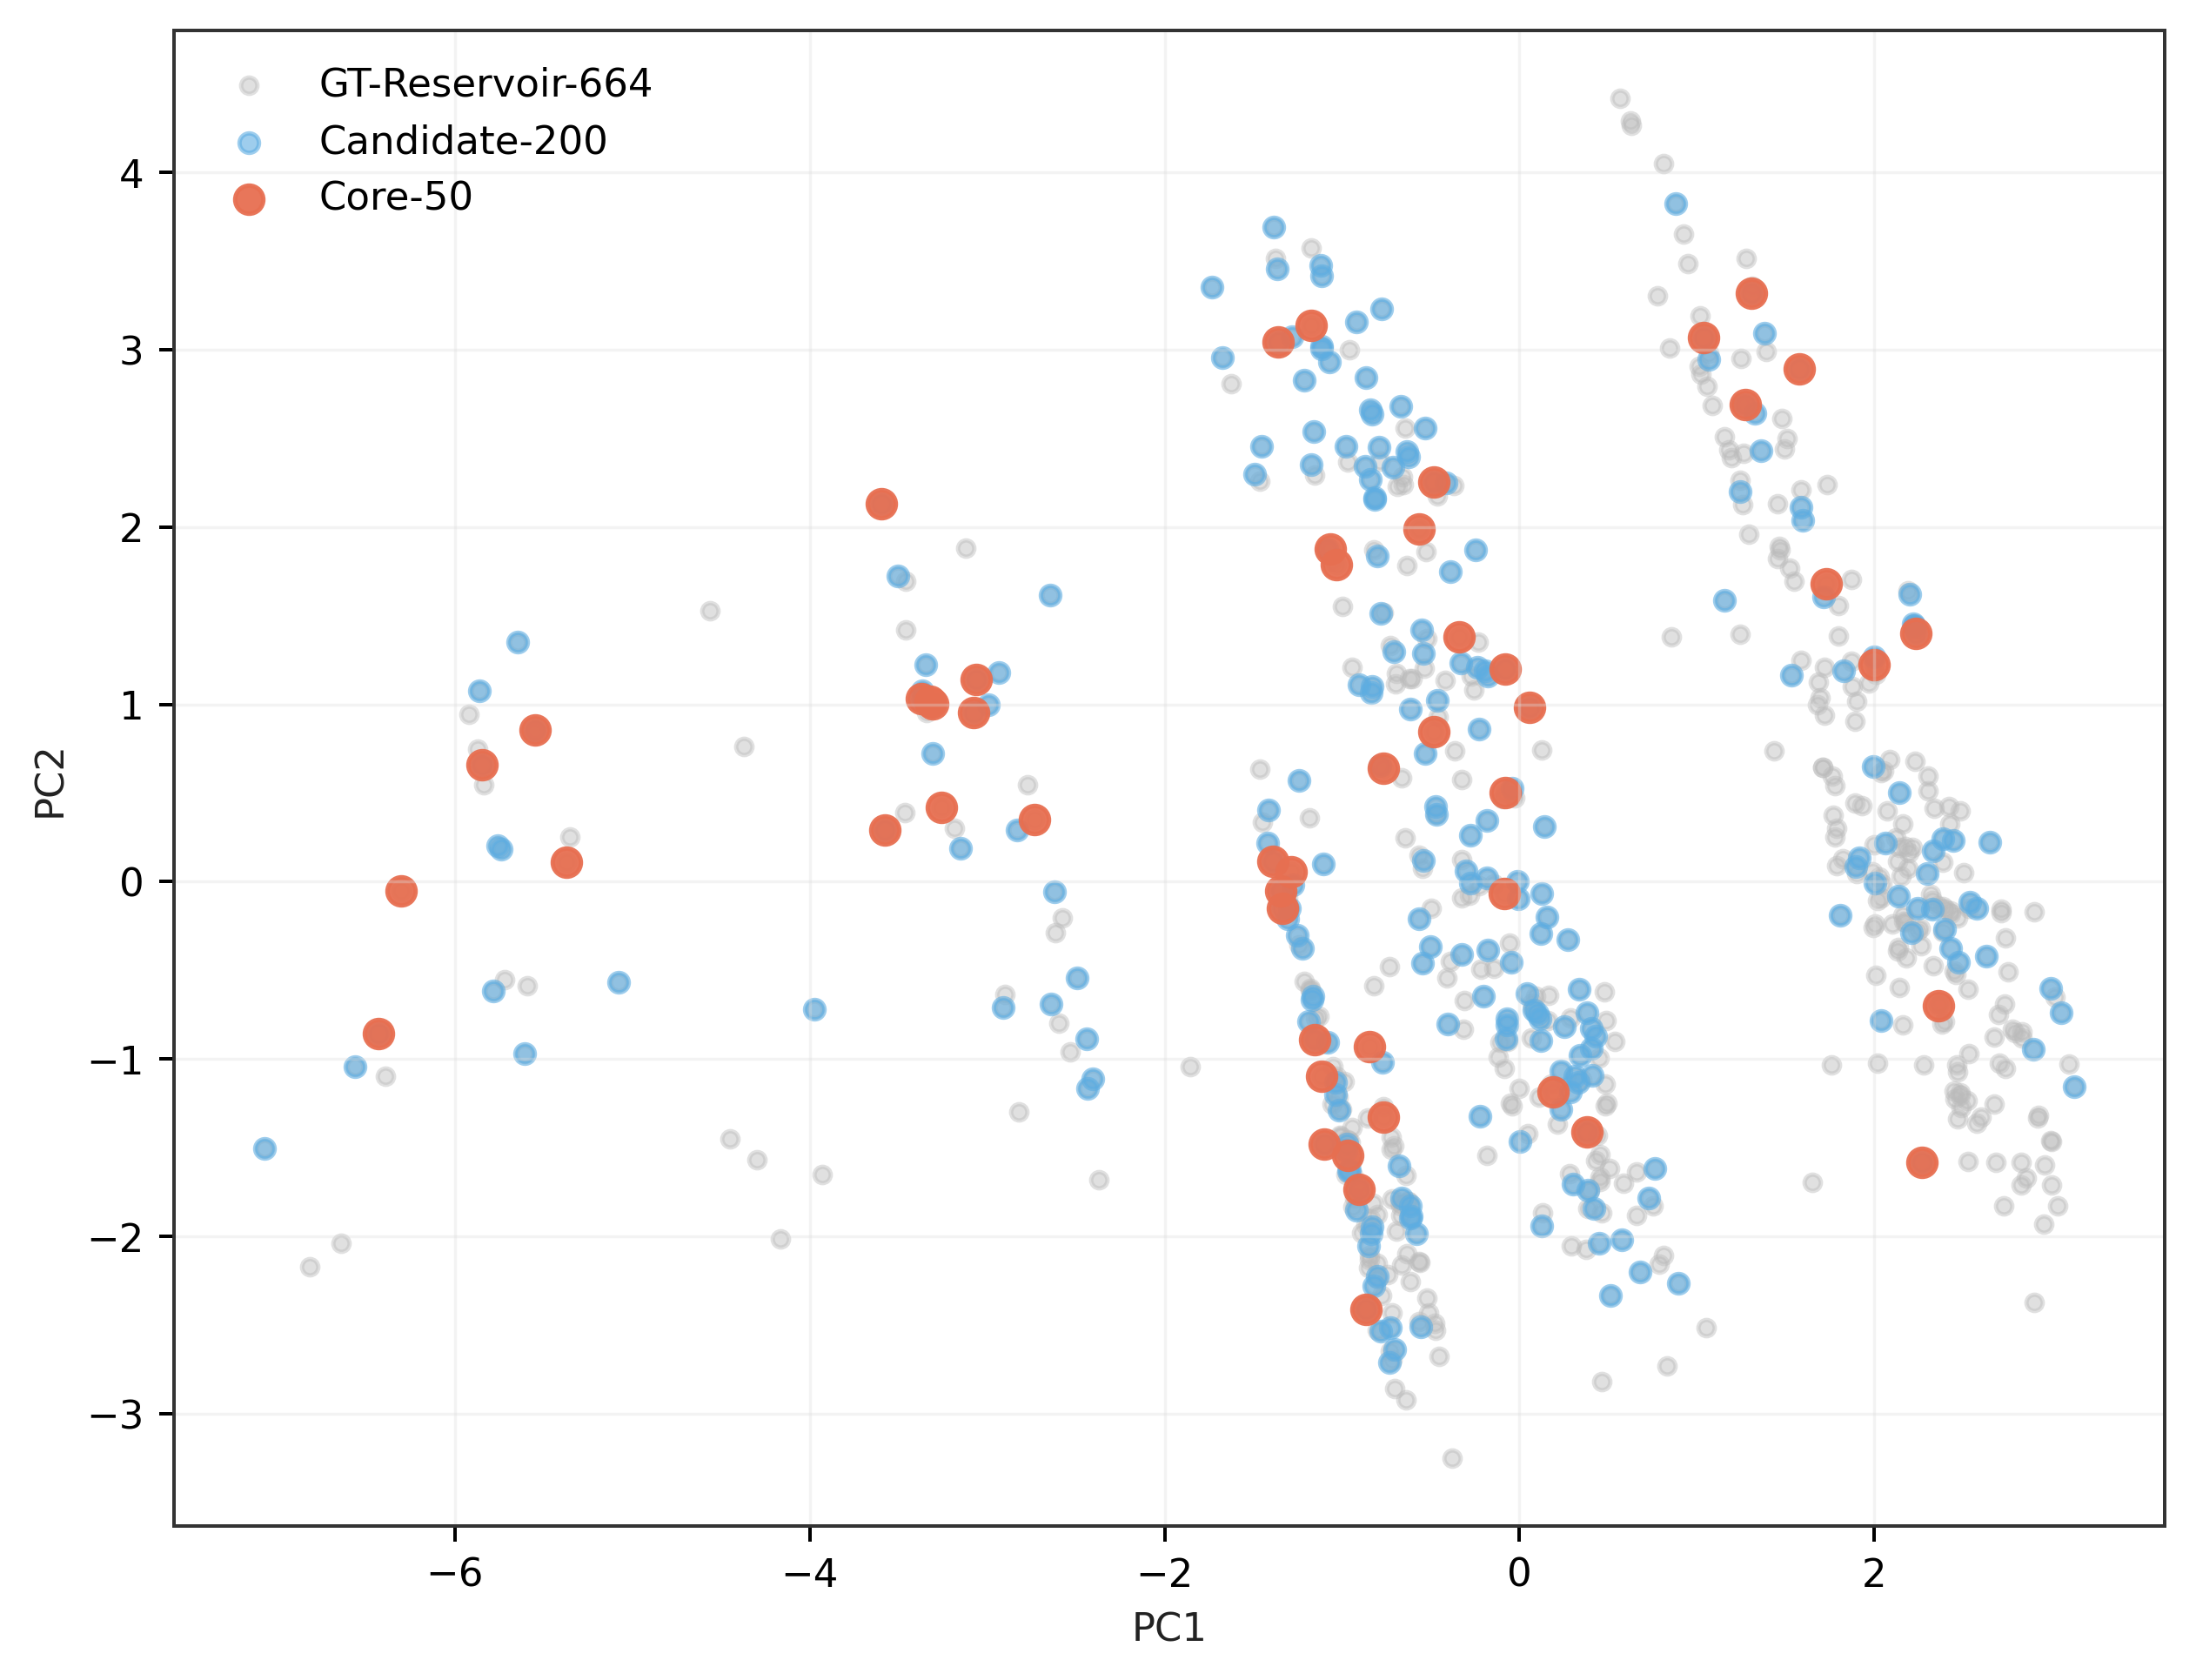
\includegraphics[width=0.82\linewidth]{imgs/Article/figure10_core50_coverage_map}
\caption{\textbf{\core{} coverage over \reservoir{}.} \core{} coverage over the reservoir-derived structural and Probe-4 response profile. The selected subset remains compact, but it covers the main family, difficulty, failure-mode, and response-pattern regions rather than collapsing into a single high-gap corner.}
\label{fig:appendix-core50-coverage-map}
\end{figure}

\begin{figure}[p]
\centering
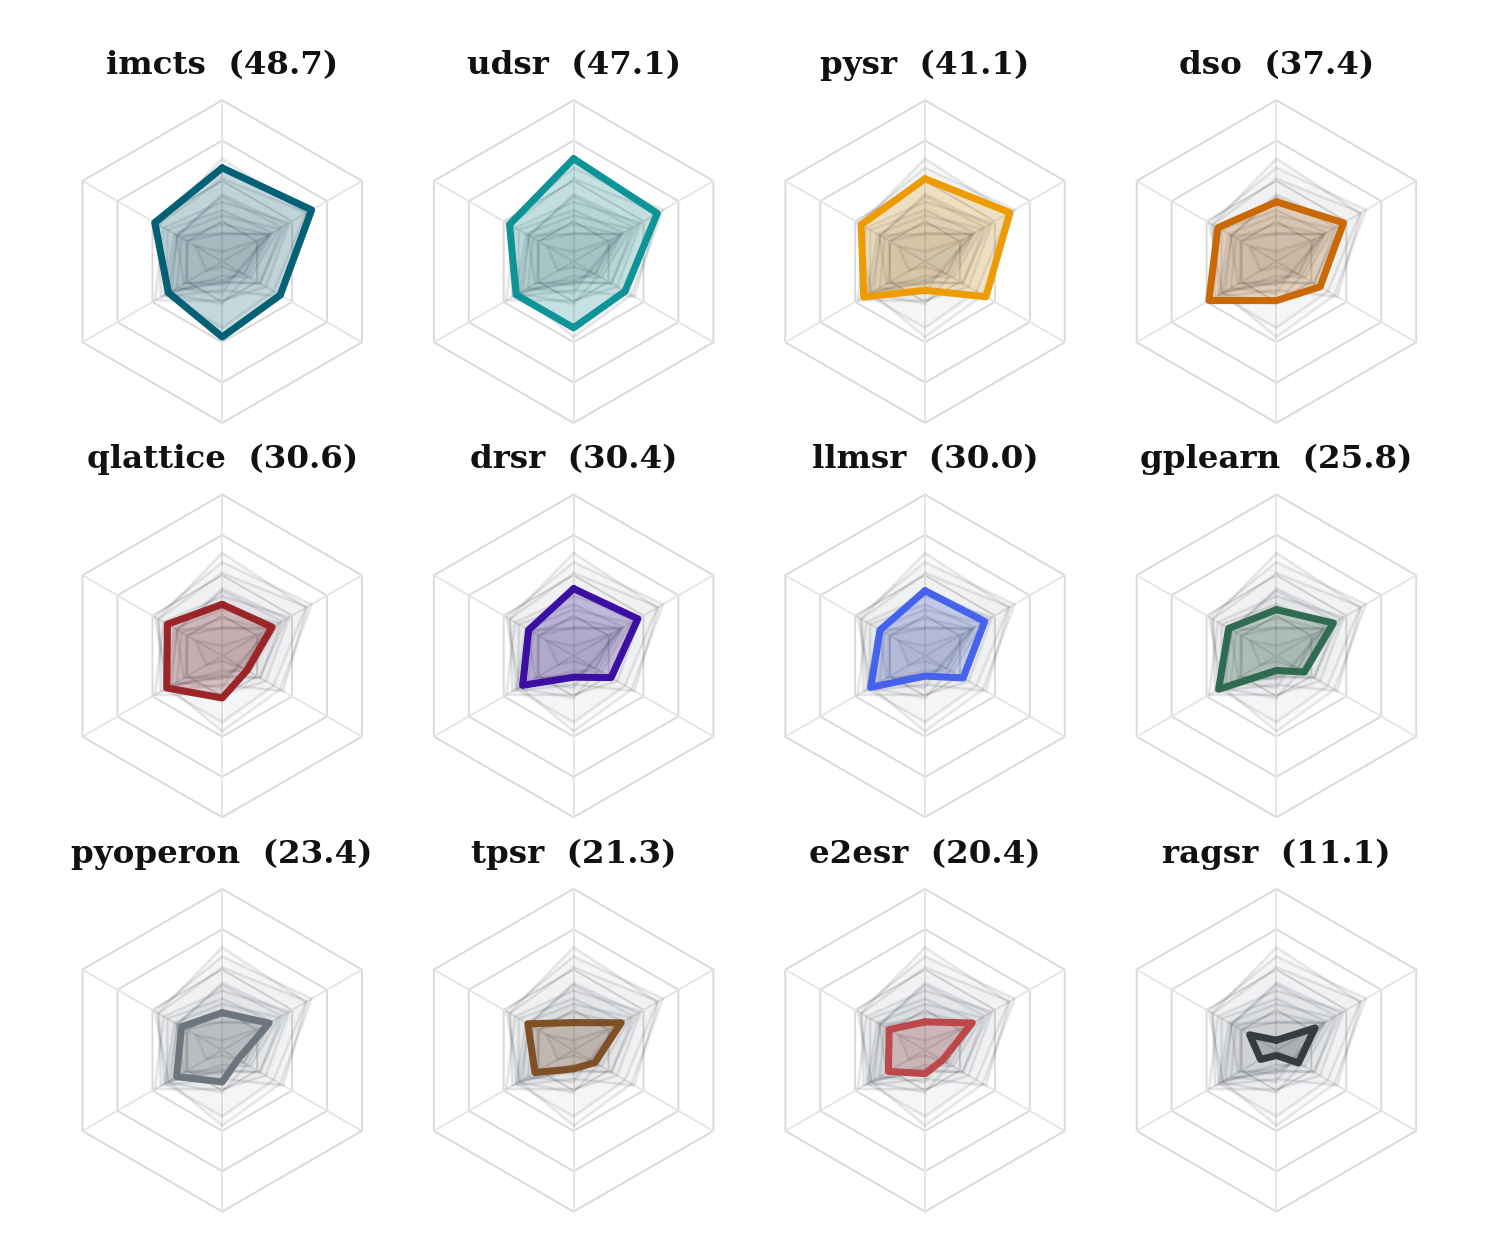
\includegraphics[width=0.86\linewidth]{imgs/Article/fig_hexagon_small_multiples_neurips}
\caption{\textbf{Per-algorithm clean-track profiles.} The small multiples make the same point as the main heatmap at algorithm level: similar OOD rankings can still hide differences in symbolic fidelity, efficiency, and effective stability.}
\label{fig:appendix-hexagon-small-multiples}
\end{figure}

\begin{figure}[p]
\centering
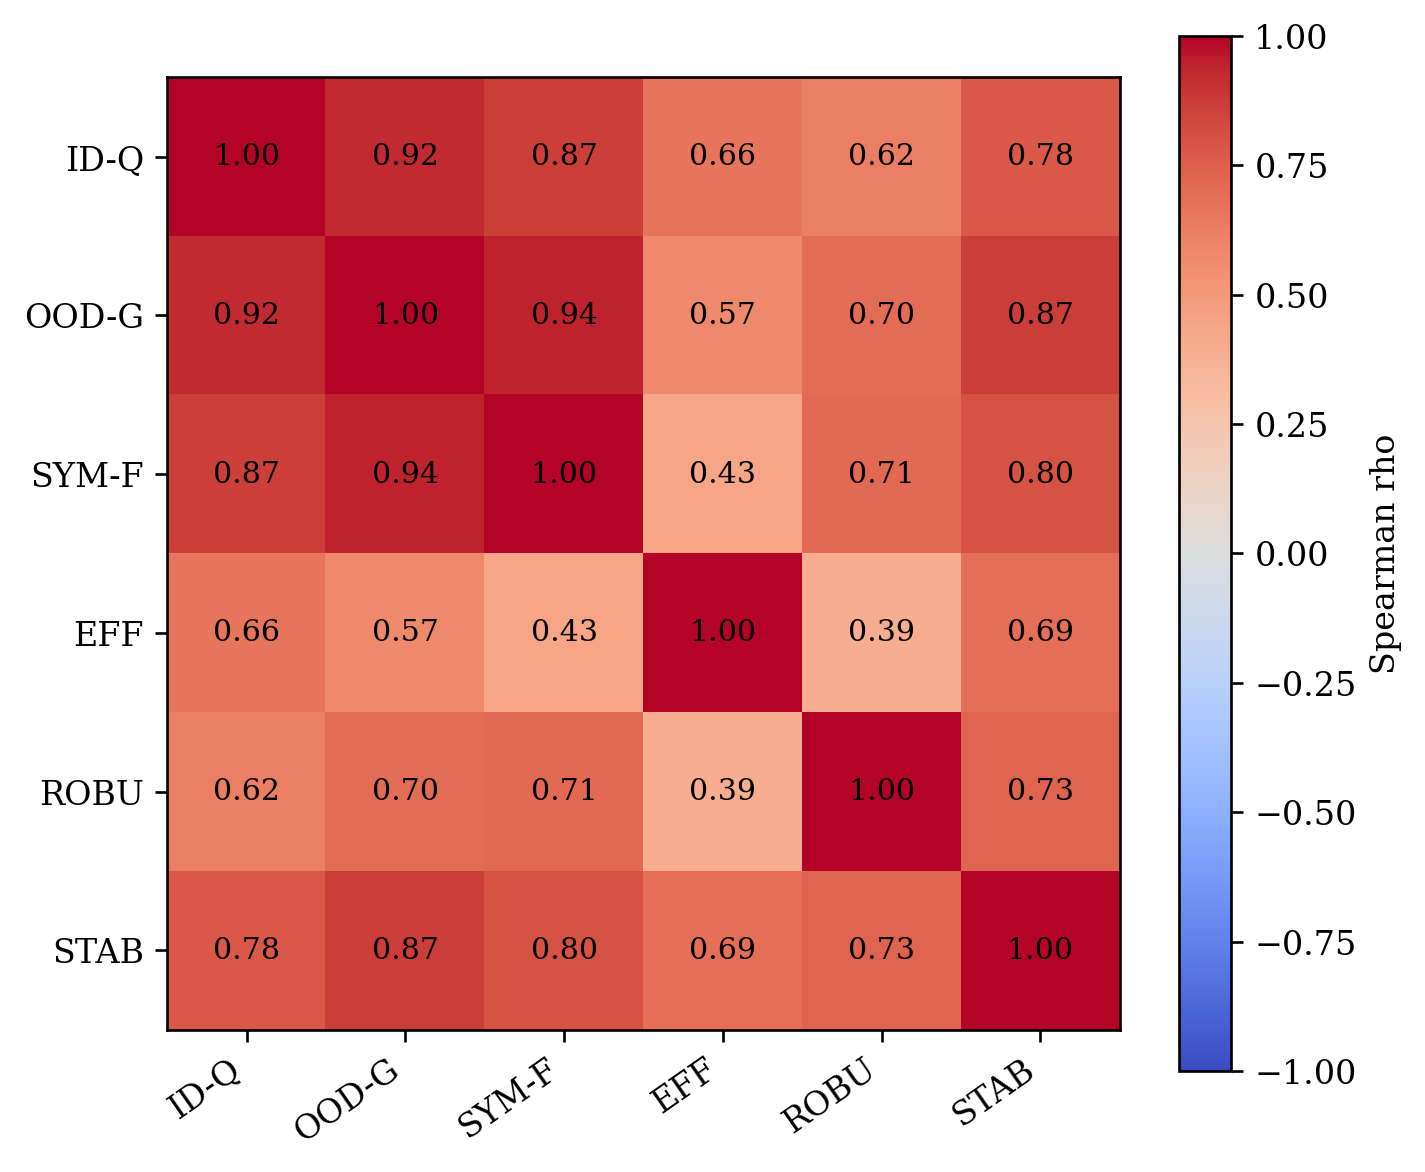
\includegraphics[width=0.76\linewidth]{imgs/Article/figure29_axis_correlation_matrix}
\caption{\textbf{Clean-track axis correlation structure.} The axes and robustness extension are related, but they do not collapse into a single numerical-error score, motivating separate reporting rather than one opaque aggregate.}
\label{fig:appendix-axis-correlation}
\end{figure}

\begin{figure}[p]
\centering
\begin{minipage}{0.48\linewidth}
\centering
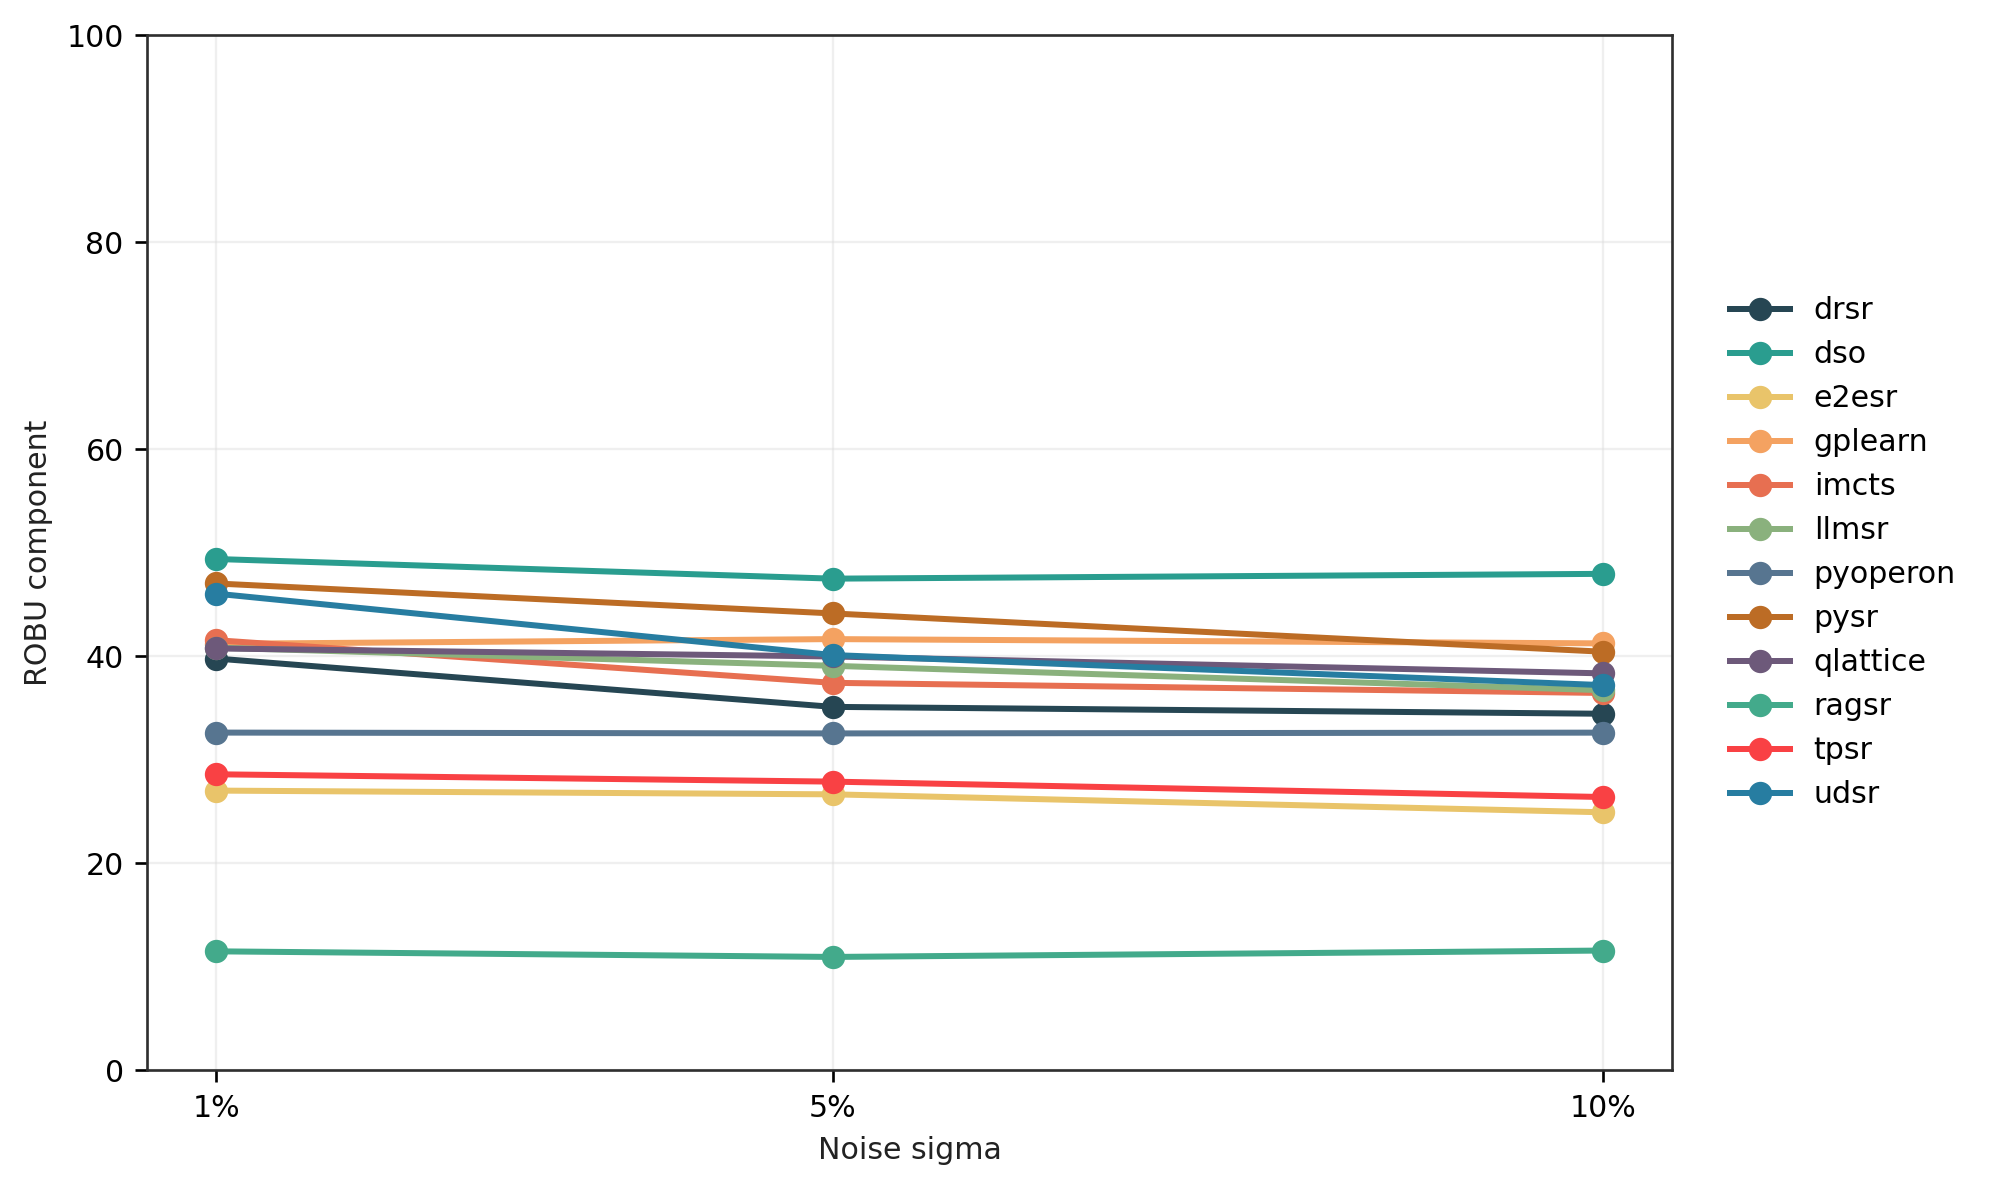
\includegraphics[width=\linewidth]{imgs/Article/figure25_noise_robustness_curve}
\end{minipage}
\hfill
\begin{minipage}{0.48\linewidth}
\centering
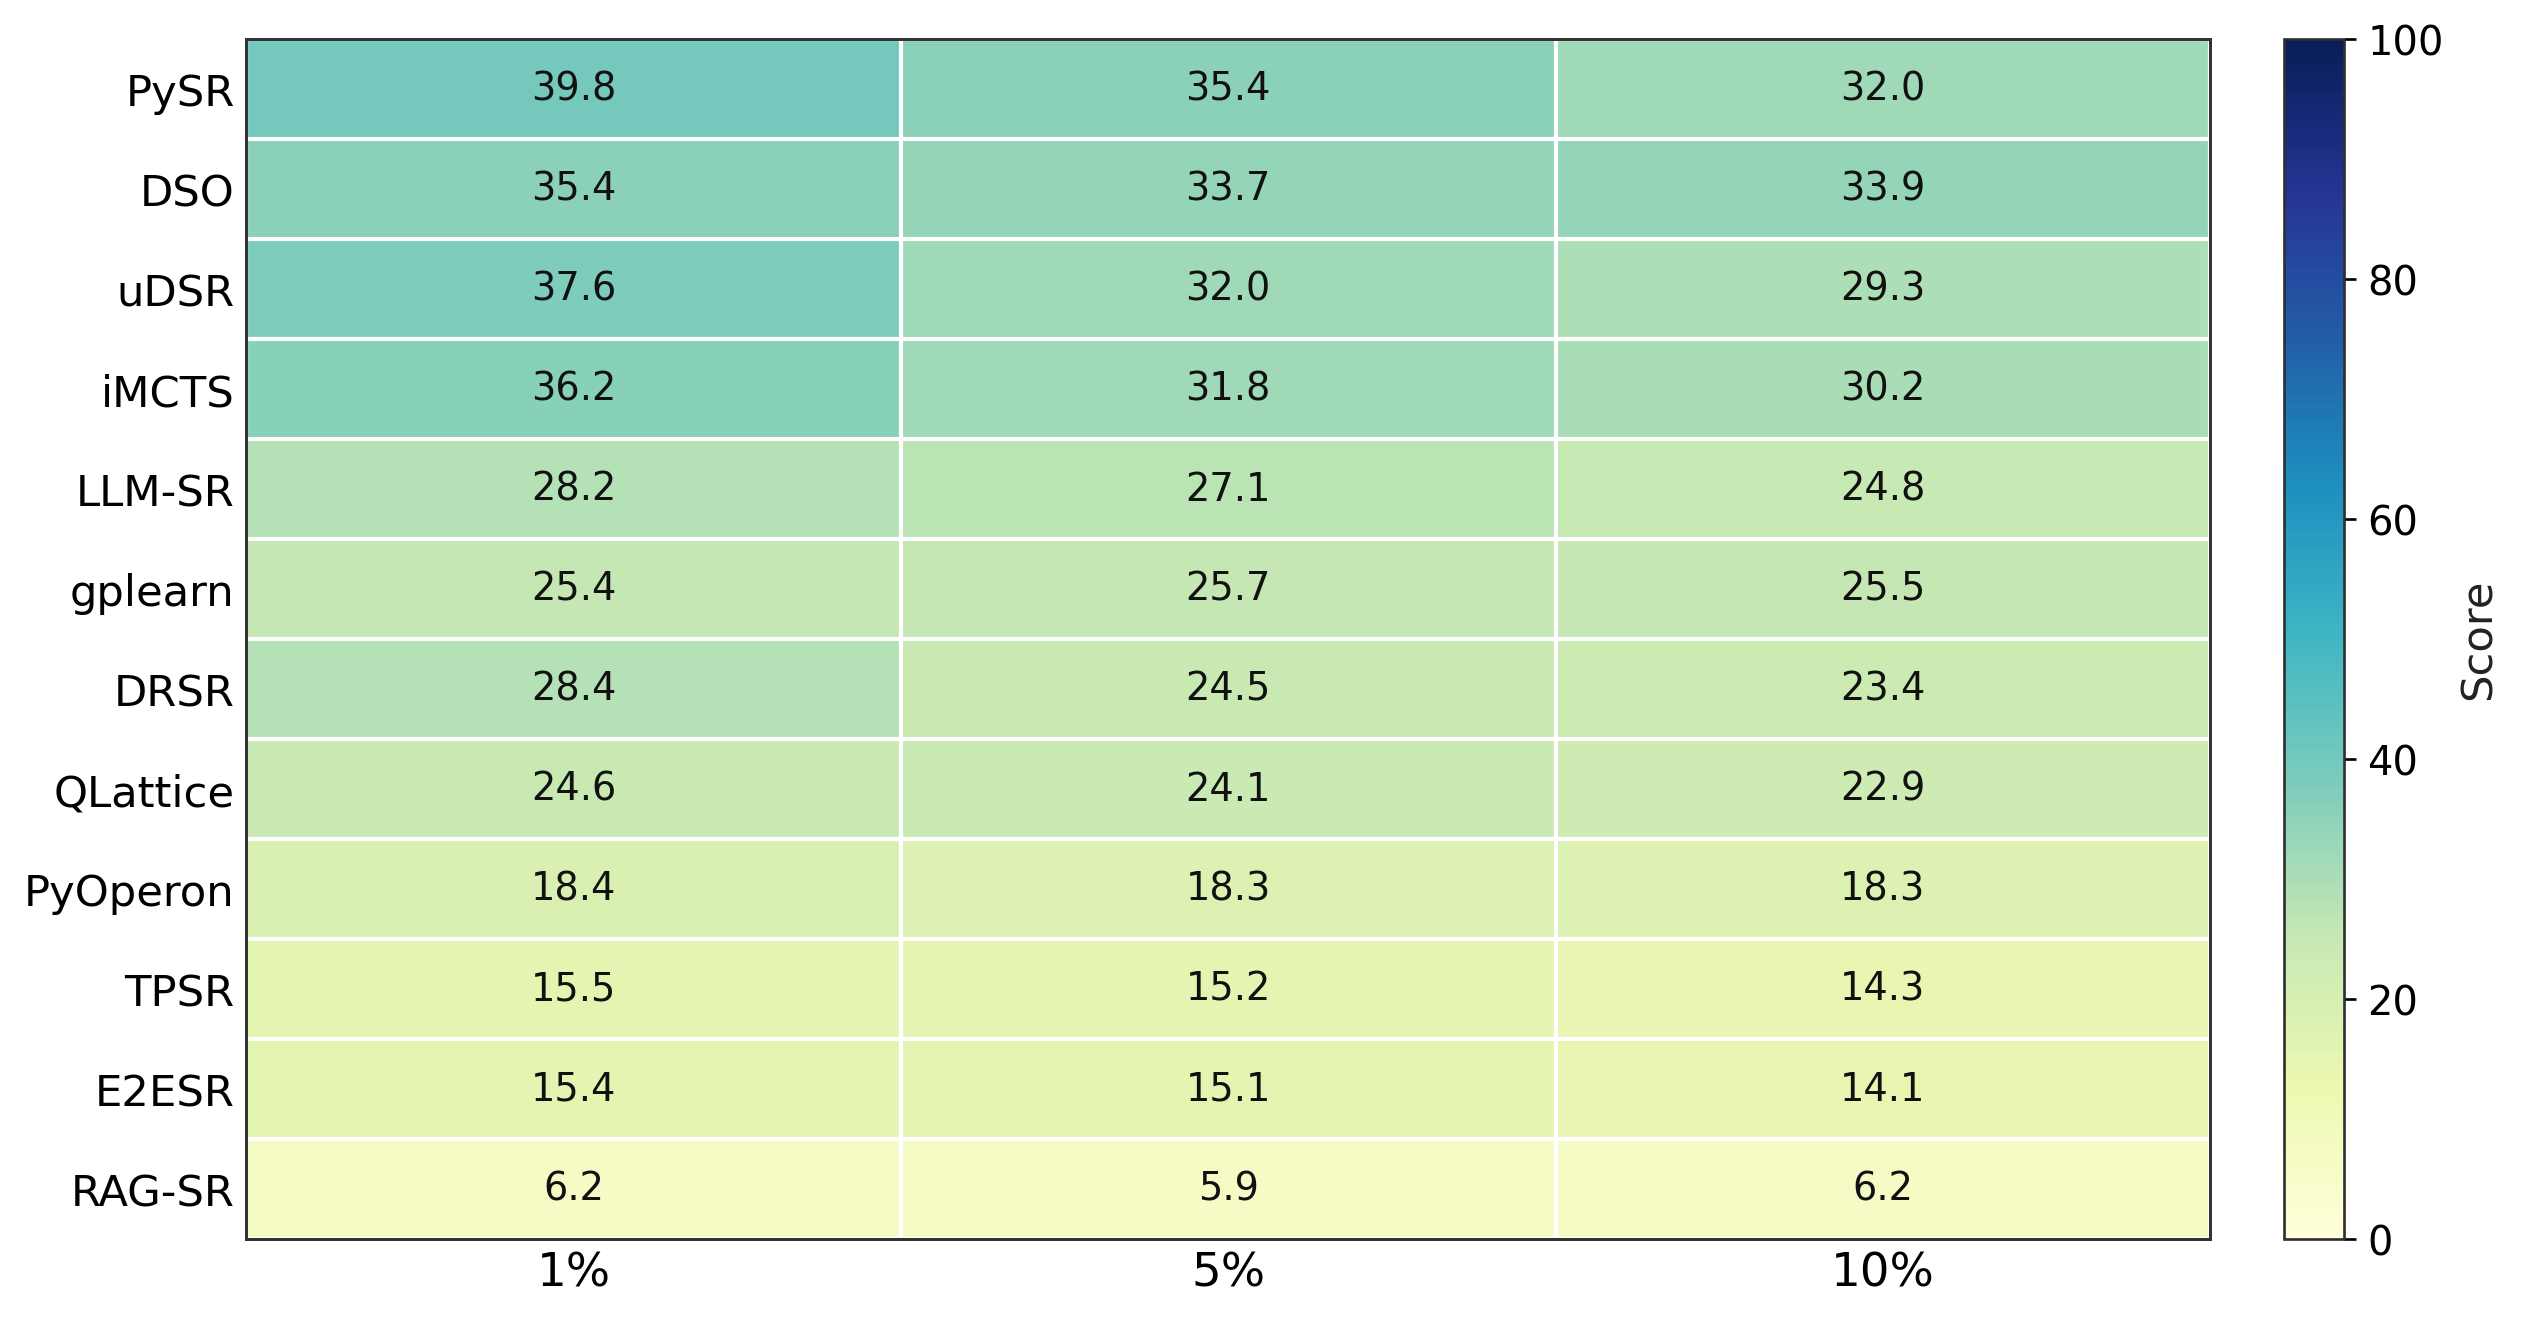
\includegraphics[width=\linewidth]{imgs/Article/figure26_noise_quality_heatmap}
\end{minipage}
\caption{\textbf{Noisy-training robustness extension.} Left: robustness curves summarize clean-test quality under increasing training noise. Right: the noise-quality heatmap shows which algorithms retain usable formulas under the standardized noisy-track protocol.}
\label{fig:appendix-robustness-extension}
\end{figure}


\clearpage
\setcounter{figure}{0}
\renewcommand{\thefigure}{E.\arabic{figure}}
\renewcommand{\theHfigure}{appendixE.\arabic{figure}}
\section{Diagnostic Profiles of Evaluated Algorithms}
\label{app:algorithm-diagnostics}

A single leaderboard rank does not explain why a symbolic-regression method fails. \arena{} records output validity, metric completeness, numerical quality, OOD behavior, symbolic-fidelity artifacts, complexity, seed-level behavior, and minute-level search traces. This makes it possible to diagnose failures at a finer granularity than a single OOD-NMSE column. The goal of this appendix is not to declare an algorithm universally good or bad, but to summarize which failure modes are exposed by \core{} under the \arena{} protocol.

\paragraph{Failure taxonomy.}
We use seven diagnostic categories. \emph{Numerical underfitting} denotes failure to obtain good ID or validation fit. \emph{OOD degradation} denotes a large drop from ID quality to OOD quality, suggesting shortcut expressions or poor extrapolation. \emph{Symbolic mismatch} denotes low expression-level agreement with the ground-truth formula even when numerical error is low. \emph{Inefficient search} denotes strong final performance but slow time-to-threshold or low anytime AUC. \emph{Premature stagnation} denotes early plateauing of best-so-far quality. \emph{Seed instability} denotes large seed-to-seed variance in numerical score, structure, or success rate. \emph{Invalid or incomplete output} denotes missing, unparsable, timed-out, or metric-incomplete artifacts.

These categories are not mutually exclusive. For example, a method may be numerically strong but symbolically mismatched, or produce valid expressions but fail complete ID/OOD metric evaluation. \Cref{fig:hexagon-heatmap,fig:appendix-hexagon-small-multiples,fig:appendix-axis-correlation,fig:appendix-robustness-extension} provide the corresponding multi-axis and robustness diagnostics. The cards below use the clean \core{} leaderboard statistics reported in the main text: each algorithm has 250 runs, and lower penalized OOD log NMSE is better.

\begin{center}
\small
\textbf{Table D.1:} Algorithm-level diagnostic summary from the clean \core{} leaderboard.

\vspace{0.4em}
\resizebox{\linewidth}{!}{%
\begin{tabular}{llrrrp{0.30\linewidth}}
\toprule
\textbf{Algorithm} & \textbf{Paradigm} & \textbf{Valid} & \textbf{Metric} & \textbf{OOD log} & \textbf{Primary diagnostic questions} \\
 & & \textbf{rate} & \textbf{complete} & \textbf{NMSE} & \\
\midrule
uDSR & neural-guided SR & 1.000 & 1.000 & $-5.646$ & Symbolic equivalence and seed-level structural consistency despite strong numerical quality \\
iMCTS & tree search / MCTS & 1.000 & 0.968 & $-3.960$ & Metric-completion gaps, time-to-threshold behavior, and symbolic mismatch \\
PySR & evolutionary GP & 1.000 & 0.960 & $-3.055$ & OOD shortcuts, expression complexity, and low-NMSE non-equivalence \\
DSO & RL / policy search & 1.000 & 0.972 & $-2.458$ & Reward-driven exploration limits, operator recovery, and seed variance \\
DRSR & LLM/hybrid SR & 1.000 & 1.000 & $-2.087$ & OOD degradation, refinement quality, and generated-structure mismatch \\
LLM-SR & LLM-assisted SR & 1.000 & 0.992 & $-1.420$ & Context sensitivity, prior mismatch, and post-generation fitting limits \\
gplearn & classical GP & 1.000 & 1.000 & $-1.207$ & Under-exploration, bloat, and OOD degradation \\
QLattice & graph/evolutionary SR & 0.980 & 0.972 & $-0.780$ & Distinguishing output-health failures from algorithmic OOD failures \\
TPSR & transformer/planning SR & 1.000 & 0.996 & $0.896$ & Pretraining-distribution mismatch and weak OOD transfer \\
PyOperon & evolutionary GP & 0.984 & 0.840 & $1.079$ & Metric incompleteness, invalid-prone tasks, and weak penalized OOD quality \\
E2ESR & end-to-end neural SR & 1.000 & 0.800 & $2.891$ & Metric-completion failures and unreliable competitive evaluation \\
RAG-SR & retrieval/LLM-assisted SR & 1.000 & 0.964 & $3.788$ & Retrieval mismatch, generated-expression quality, and OOD degradation \\
\bottomrule
\end{tabular}}
\end{center}

\paragraph{How the diagnostic evidence is computed.}
Table D.2 converts the final-result archive into interpretable failure indicators. \emph{Wins} counts the number of datasets on which an algorithm has the best five-seed median OOD log NMSE among the 12 methods. \emph{Good OOD} counts datasets with five-seed median OOD log NMSE below $-2$; \emph{bad OOD} counts datasets above $2$; and \emph{gap$>2$} counts datasets whose median OOD log NMSE exceeds median ID log NMSE by more than two log units. \emph{Miss} is the number of run-level artifacts, out of 250, for which the final result is not metric-complete. Exact-equivalence rates come from the formal symbolic-fidelity pass, which combines CAS simplification, independent numeric-equivalence probes, tree similarity, variable F1, and operator F1. These indicators intentionally mix output health, numerical behavior, symbolic recovery, and anytime efficiency, because no single column explains failures.

\begin{center}
\small
\textbf{Table D.2:} Evidence used for algorithm-level failure diagnosis. Counts are over 50 datasets unless otherwise stated.

\vspace{0.4em}
\resizebox{\linewidth}{!}{%
\begin{tabular}{lrrrrrrrp{0.31\linewidth}}
\toprule
\textbf{Algorithm} & \textbf{Wins} & \textbf{Good} & \textbf{Bad} & \textbf{Gap} & \textbf{Miss} & \textbf{Exact} & \textbf{EFF} & \textbf{Diagnostic evidence} \\
 & & \textbf{OOD} & \textbf{OOD} & \textbf{$>2$} & \textbf{/250} & \textbf{equiv.} & & \\
\midrule
uDSR & 11 & 33 & 1 & 13 & 0 & 24.0\% & 41.0 & Strong numerical recovery, but OOD gaps and modest equivalence rate require symbolic checks \\
iMCTS & 13 & 27 & 11 & 8 & 8 & 30.8\% & 46.8 & Strong OOD and efficiency profile, plus a long-tail of difficult OOD cases \\
PySR & 7 & 29 & 11 & 8 & 10 & 34.0\% & 17.8 & Highest formal \symf{} but slow anytime behavior and long-tail metric failures \\
DSO & 7 & 13 & 1 & 6 & 7 & 18.0\% & 24.2 & Healthy RL baseline with symbolic shortcut cases despite good numerical fit \\
DRSR & 9 & 20 & 4 & 11 & 0 & 12.0\% & 13.2 & Complete artifacts; failures concentrate in refinement, OOD gaps, and low symbolic recovery \\
LLM-SR & 0 & 15 & 5 & 14 & 4 & 12.8\% & 12.5 & Evaluable outputs but no dataset wins, low efficiency, and context-sensitive OOD gaps \\
gplearn & 0 & 9 & 0 & 5 & 0 & 8.0\% & 9.0 & Stable classical GP baseline; failures are search expressivity and symbolic mismatch \\
QLattice & 0 & 12 & 4 & 16 & 7 & 4.8\% & 26.1 & Fast but gap-prone; output health and OOD retention must be separated \\
TPSR & 1 & 4 & 8 & 7 & 1 & 0.4\% & 11.5 & Valid outputs but weak symbolic recovery and pretraining-distribution transfer \\
PyOperon & 1 & 6 & 10 & 11 & 40 & 0.0\% & 19.7 & Severe metric-completeness issue and no formal equivalence under this protocol \\
E2ESR & 1 & 10 & 18 & 9 & 50 & 0.0\% & 14.5 & Valid artifacts often fail complete evaluation; poor OOD and zero exact recovery \\
RAG-SR & 0 & 1 & 27 & 9 & 9 & 1.6\% & 3.2 & Mostly numerical underfitting rather than missing-output failure; weakest efficiency \\
\bottomrule
\end{tabular}}
\end{center}

\paragraph{Representative symbolic shortcut.}
The symbolic-fidelity pass exposes low-error but non-equivalent expressions. We report \texttt{Nguyen-9} because it is a repeated low-NMSE non-equivalence pattern found by the audit, not a hand-selected single failure. The ground-truth expression is $\sin(x_0)+\sin(x_1^2)$, while several low-NMSE predictions simplify to $\sin(x_0)+\sin(x_0^2)$. This shortcut appears in five DSO seeds, two gplearn seeds, and one PySR seed. Its ID and OOD NMSE are near machine precision, but the formal \symf{} score is only $0.424$. This case illustrates why \arena{} does not treat numerical fit alone as symbolic recovery.

\subsection{Per-Algorithm Diagnostic Cards}

\paragraph{uDSR.}
uDSR is the strongest numerical method under the penalized OOD leaderboard: it wins 11 datasets, has no metric-incomplete runs, and reaches good OOD quality on 33 of 50 datasets. Its diagnostic weakness is not artifact health, but symbolic and extrapolation fidelity. Its exact-equivalence rate is 24.0\%, below PySR and iMCTS, and 13 datasets have an OOD-ID gap above two log units. \arena{} therefore treats uDSR as a strong numerical baseline whose outputs still require \symf{} and seed-level structural checks.

\paragraph{iMCTS.}
iMCTS has the strongest clean-track OOD/efficiency profile and wins the largest number of datasets (13 of 50). It has the best \oodg{} and EFF values among the evaluated methods, which indicates that tree-search behavior is both accurate and comparatively efficient under the one-hour protocol. The failure pattern is long-tailed: although 27 datasets have good OOD quality, 11 have bad OOD quality, and 8 of 250 runs are not metric-complete. The diagnostic question is therefore not whether iMCTS is competitive, but why its search occasionally produces difficult-to-evaluate or OOD-fragile expressions.

\paragraph{PySR.}
PySR is the strongest symbolic-fidelity method in the formal pass, with the highest \symf{} and exact-equivalence rate (34.0\%). It also has good OOD quality on 29 datasets. Its main diagnostic weaknesses are cost and tail behavior: EFF is only 17.8, 10 runs are not metric-complete, and 11 datasets have bad OOD quality despite strong aggregate performance. PySR therefore looks like a high-quality final evaluator but not always an efficient anytime baseline.

\paragraph{DSO.}
DSO is a healthy RL/policy-search baseline: it wins 7 datasets and has only 7 metric-incomplete runs. Its failures are more symbolic than infrastructural. The low-NMSE non-equivalence audit finds five DSO seeds on \texttt{Nguyen-9} with near-perfect numerical error but a wrong variable structure. This is consistent with reward-driven exploration: a policy can discover a numerically excellent shortcut without recovering the intended formula.

\paragraph{DRSR.}
DRSR has complete artifact health and wins 9 datasets, so its mid-tier leaderboard position should not be explained away as missing outputs. Instead, the failure modes are refinement quality, OOD degradation, and symbolic mismatch. It has 20 good-OOD datasets, but 11 datasets have an OOD-ID gap above two log units, and exact equivalence is only 12.0\%. This suggests that generated structures are often executable but not consistently ground-truth equivalent.

\paragraph{LLM-SR.}
LLM-SR produces evaluable outputs but does not win any dataset under the five-seed median OOD criterion. It has 15 good-OOD datasets, but 14 datasets have OOD-ID gaps above two log units and its EFF score is low (12.5). This pattern suggests that the method can generate plausible formulas, but the formal \core{} protocol still exposes context sensitivity, OOD degradation, and post-generation fitting limits. The result should be interpreted under the recorded prompt/context contract, rather than as a context-free statement about all LLM-assisted SR.

\paragraph{gplearn.}
gplearn is a stable classical GP baseline: all 250 runs are valid and metric-complete, and none of the datasets have bad OOD medians above 2. Its weakness is not reliability but competitiveness. It wins no dataset, reaches good OOD quality on only 9 datasets, and exact equivalence is 8.0\%. The \texttt{Nguyen-9} shortcut also appears in two gplearn seeds. Thus gplearn is useful as a clean classical baseline, but its failures are dominated by under-exploration and symbolic mismatch.

\paragraph{QLattice.}
QLattice is fast, with median runtime far below the one-hour methods, but its diagnostic profile is gap-prone. It has 5 no-valid-output runs, 7 metric-incomplete runs, and no dataset wins. It still reaches good OOD quality on 12 datasets, but 16 datasets have OOD-ID gaps above two log units. This means its failures should not be reduced to output-health problems: even when expressions are valid, OOD retention and symbolic recovery remain limiting factors.

\paragraph{TPSR.}
TPSR has almost complete metric health, but weak \idq{}, \oodg{}, and symbolic recovery. It wins one dataset, reaches good OOD quality on only 4 datasets, and exact equivalence is 0.4\%. Since only one run is metric-incomplete, the primary diagnosis is not wrapper failure. The more plausible failure mode is proposal-distribution mismatch: the pretrained or learned symbolic prior does not transfer cleanly to many \core{} tasks under the fixed one-hour adaptation budget.

\paragraph{PyOperon.}
PyOperon shows the clearest output-health warning among the evolutionary methods. It has 4 no-valid-output runs and 40 metric-incomplete runs, and formal exact equivalence is 0.0\%. At the same time, it still wins one dataset and reaches good OOD quality on 6 datasets, so it is not simply unusable. The diagnosis is that PyOperon is a useful stress-test probe for invalid-prone and difficult tasks, but its leaderboard score must retain explicit metric-completeness penalties.

\paragraph{E2ESR.}
E2ESR illustrates the distinction between valid artifacts and complete evaluation. All 250 runs produce valid artifacts, but 50 are not metric-complete. It reaches good OOD quality on 10 datasets and wins one dataset, but 18 datasets have bad OOD medians and exact equivalence is 0.0\%. The failure mode is therefore not absence of output; it is that the produced output often fails to yield robust, competitive ID/OOD and symbolic evaluation under the shared evaluator.

\paragraph{RAG-SR.}
RAG-SR ranks last under the penalized OOD leaderboard and wins no dataset. It has 8 timed-out runs and 9 metric-incomplete runs, but its dominant failure is numerical quality rather than missing output: 42 datasets have OOD medians above 0 and 27 are above 2. Its clean-track \idq{}, \oodg{}, EFF, and STAB are all weak relative to the 12-method panel. Under the current wrapper and context protocol, the retrieved or generated structures do not reliably match the \core{} equations.

\subsection{Cross-Algorithm Patterns}

The diagnostic cards show that SR algorithms fail in qualitatively different ways. uDSR, iMCTS, and PySR are strong numerically, but still require symbolic-equivalence and long-tail OOD checks. DSO, DRSR, and LLM-SR often produce executable formulas, yet reveal different mixtures of shortcutting, refinement limits, and OOD degradation. gplearn is reliable but rarely wins. QLattice is fast but gap-prone. TPSR, E2ESR, PyOperon, and RAG-SR expose different forms of distribution mismatch, metric incompleteness, or numerical underfitting. These distinctions justify \arena{}'s multi-axis design: a single OOD-NMSE ranking cannot capture the diagnostic structure of modern SR systems.

The current appendix intentionally reports algorithm-level patterns rather than per-dataset blame. The released trace archive supports a stricter follow-up table with representative cases of OOD shortcutting, low-NMSE non-equivalence, seed instability, timeout/no-valid-output, and complexity growth. Such case tables should be generated mechanically from the released \texttt{result.json} and minute-level progress artifacts to avoid cherry-picking.


\clearpage
\setcounter{figure}{0}
\renewcommand{\thefigure}{F.\arabic{figure}}
\renewcommand{\theHfigure}{appendixF.\arabic{figure}}
\section{Evaluated Baselines and Integration Notes}
\label{app:evaluated-baselines}

This appendix documents the 12 algorithms used in the \core{} leaderboard. The purpose is not to claim that every upstream method is reimplemented with all optional research features enabled. Instead, \arena{} treats each baseline as a fixed, executable evaluation target with an explicit wrapper contract, environment, operator set, wall-clock budget, seed interface, progress logging, and artifact schema. This makes the leaderboard auditable: if a result differs from an upstream paper, the difference can be traced to data selection, budget, prompt context, operator set, pretrained-model distribution, wrapper variant, or postprocessing.

\begin{center}
\small
\textbf{Table E.1:} Baseline panel used in the \core{} leaderboard.

\vspace{0.4em}
\resizebox{\linewidth}{!}{%
\begin{tabular}{llllp{0.38\linewidth}}
\toprule
Method & Paradigm & Main reference & \arena{} role & Integration note \\
\midrule
gplearn & classical GP & software baseline & classical GP sanity baseline & scikit-learn-style GP with protected functions and one-hour budget \\
PyOperon & evolutionary GP & \citet{burlacu2020operon} & modern GP / fast C++ baseline & Operon/PyOperon wrapper with local search and explicit metric-completeness accounting \\
PySR & evolutionary GP & \citet{cranmer2023pysr} & strong general-purpose SR baseline & SymbolicRegression.jl backend through PySR; Julia cache and timeout recovery are part of the contract \\
QLattice & graph/evolutionary SR & \citet{brolos2021feyn} & graph-structured SR baseline & Feyn/QLattice community interface; BIC-oriented model selection and output-health accounting \\
RAG-SR & retrieval / evolutionary hybrid & \citet{zhang2025ragsr} & retrieval-augmented GP-family baseline & EvolutionaryForest-backed RAG-SR wrapper with official-style target encoding defaults \\
DSO & RL / policy search & \citet{petersen2021dsr} & pure RL symbolic-policy baseline & risk-seeking policy-gradient controller with explicit operator and prior configuration \\
uDSR & neural-guided hybrid & \citet{landajuela2022unified} & DSO-plus-hybrid neural-guided baseline & benchmarked as a uDSR-trunk variant with DSO controller, LINEAR/poly token, and GP-meld \\
iMCTS & MCTS / tree search & \citet{huang2025imcts} & explicit tree-search baseline and Probe-4 member & improved MCTS with real-constant token and GP-style state jumps \\
E2ESR & end-to-end transformer & \citet{kamienny2022end} & pretrained neural SR baseline & E2E transformer predicts complete expressions and refines constants under fixed input-point limits \\
TPSR & transformer + planning & \citet{shojaee2023tpsr} & transformer-planning baseline & E2E backbone plus lookahead/MCTS-style planning and candidate filtering \\
LLM-SR & LLM-assisted SR & \citet{shojaee2025llmsr} & LLM scientific-programming baseline & LLM-generated equation programs with BFGS-style parameter fitting and recorded prompt contract \\
DRSR & LLM + dual reasoning & \citet{wang2025drsr} & data-aware LLM-reflection baseline & LLM generation augmented with data analysis, experience buffer, and iterative reflection \\
\bottomrule
\end{tabular}}
\end{center}

\paragraph{gplearn.}
gplearn is a classical genetic-programming SR implementation with a scikit-learn-style interface. It evolves expression programs using crossover, subtree mutation, hoist mutation, point mutation, tournament selection, and parsimony pressure. \arena{} includes gplearn because it is a stable and interpretable classical GP baseline: it is not expected to dominate modern SR systems, but it provides a useful lower-complexity reference point for output validity, search stability, and symbolic mismatch. In our wrapper, gplearn receives the same explicit data contract as the other methods, including feature count, feature names, target name, seed, and one-hour timeout. The configured operator set includes arithmetic, protected division, square root, logarithm, sine, and cosine, making the baseline broad enough for elementary-equation tasks while still representing a conventional GP search process.

\paragraph{PyOperon.}
PyOperon exposes the Operon C++ symbolic-regression framework through Python bindings. Operon is a high-performance GP framework with linear tree encoding, scalable evolutionary search, and local parameter optimization \citep{burlacu2020operon}. \arena{} uses PyOperon as a modern evolutionary baseline and as a useful stress-test method: it can be very fast and expressive, but incomplete or unevaluable outputs must be counted explicitly rather than silently removed. The integration fixes a benchmark-level operator set including arithmetic, analytic quotient, exponential, logarithmic, trigonometric, square, square-root, constants, and variables. It also records whether the final expression is metric-complete on train, validation, ID, and OOD splits. This distinction matters because PyOperon's \core{} behavior is not only a numerical score; it also exposes metric-completeness failures under a common evaluator.

\paragraph{PySR.}
PySR is a widely used SR system built on the Julia package SymbolicRegression.jl \citep{cranmer2023pysr}. It performs evolutionary search over expression trees, combines multiple populations with migration, applies complexity penalties, and can use constraints over operators and expression nesting. \arena{} includes PySR for two reasons. First, it is a strong contemporary evolutionary baseline and therefore a natural dual-probe method for mining \candidate{}. Second, it is a practical test of infrastructure robustness because it requires a Julia backend, a persistent package cache, timeout recovery, and hall-of-fame extraction. The benchmark wrapper records best-so-far expressions and can recover evaluable candidates from PySR artifacts after budget exhaustion, so a timeout with output is treated differently from a failure to produce any expression.

\paragraph{QLattice.}
QLattice, commonly accessed through the Feyn package, searches graph-structured models that can be rendered as symbolic equations \citep{brolos2021feyn,wilstrup2021small}. It is designed for interpretable model discovery, often emphasizing compact formulas and model-selection criteria such as BIC. \arena{} includes QLattice as a graph/evolutionary SR baseline, complementary to tree-based GP and neural methods. The wrapper uses the native QLattice regression interface, passes the benchmark's numeric features under the shared data contract, and exports the selected equation into the canonical symbolic-artifact schema. Because QLattice can return no model or partial model sets on difficult tasks, validity and metric-completion fields are reported separately from numerical quality.

\paragraph{RAG-SR.}
RAG-SR is a retrieval-augmented neural symbolic-regression framework that combines retrieval over symbolic structures with evolutionary search and neural components \citep{zhang2025ragsr}. In our codebase, the operational implementation is backed by the EvolutionaryForest/RAG-SR interface, and the wrapper follows official-style defaults such as target encoding, automatic lexicase selection, external archive usage, a symbolic-library pool, and a rich primitive set including arithmetic, analytic quotient, square root, absolute-log, trigonometric, max/min, and negation. This baseline should therefore be interpreted as the fixed RAG-SR/EvolutionaryForest integration included in \arena{}, not as an unconstrained claim about every possible RAG-SR configuration. Its value in the benchmark is diagnostic: retrieval-augmented and library-guided search can fail through irrelevant retrieval, weak constant fitting, or mismatch between retrieved structures and the target equation.

\paragraph{DSO.}
Deep Symbolic Optimization / Deep Symbolic Regression learns a policy over expression tokens using risk-seeking policy gradients \citep{petersen2021dsr}. Instead of enumerating expressions with hand-coded GP operators, DSO samples programs from a neural controller and optimizes the controller toward high-reward symbolic expressions. \arena{} includes DSO as the representative pure RL/policy-search baseline. The benchmark configuration fixes the regression task, elementary operator set, reward metric, expression-length prior, repeat constraints, trigonometric and inverse priors, constant handling, batch size, entropy regularization, and one-hour budget. This makes DSO's failures interpretable as policy-search behavior rather than as wrapper ambiguity: strong cases indicate successful reward-guided exploration, while failures often reflect under-exploration, rare-operator difficulty, or numerical shortcuts.

\paragraph{uDSR.}
The unified deep symbolic regression framework combines several modules, including DSO-style controller search, neural-guided components, GP-meld, and the LINEAR/poly token \citep{landajuela2022unified}. \arena{} deliberately labels its integrated method as a \emph{uDSR-trunk variant}: it uses the DSO/uDSR source tree with the DSO controller, LINEAR/poly token, and GP-meld enabled, but does not claim to reproduce every optional full-uDSR component such as AI-Feynman-style recursive decomposition or LSPT pretraining. This naming is important for fairness. The method is included because it represents a stronger neural-guided hybrid than plain DSO while preserving a transparent execution path. Its strong \core{} performance should therefore be read as evidence for this fixed trunk variant under \arena{}, not as a universal statement about all uDSR configurations.

\paragraph{iMCTS.}
iMCTS is an improved Monte Carlo Tree Search framework for symbolic regression \citep{huang2025imcts}. It treats expression construction as tree search and adds mechanisms such as extreme bandit allocation, real-constant subspaces, and evolution-inspired state-jumping actions. \arena{} includes iMCTS both as a leaderboard method and as one of the selected non-LLM \probe{} methods, because it adds an explicit tree-search paradigm that is not covered by GP, RL, or LLM baselines. The wrapper transposes data into iMCTS's expected feature-by-sample format, passes the fixed operator set, includes the real-constant token, and exports the simplified expression plus the raw search path when available. Its diagnostics are especially useful for separating search quality from expression-evaluation completeness.

\paragraph{E2ESR.}
End-to-End Symbolic Regression with Transformers predicts complete symbolic expressions, including constants, from sampled input-output points \citep{kamienny2022end}. Unlike skeleton-first neural SR pipelines, E2ESR attempts to decode the full expression directly and then optionally refine candidates. \arena{} uses E2ESR as a pretrained neural SR baseline. The wrapper limits the number of input points and bags, refines a fixed number of decoded trees, rescales inputs when enabled, and runs under CPU-forced benchmark settings for reproducibility across the cluster. This baseline is particularly sensitive to distribution shift: if \core{} tasks differ from the synthetic pretraining distribution in variable count, operator structure, dummy variables, or OOD split design, E2ESR can return valid artifacts while still failing complete or competitive evaluation.

\paragraph{TPSR.}
TPSR extends transformer-based SR with lookahead planning, incorporating MCTS-style search into transformer decoding and allowing non-differentiable feedback such as fitting accuracy and complexity to guide candidate generation \citep{shojaee2023tpsr}. \arena{} includes TPSR as the transformer-plus-planning baseline. The integration uses the E2E pretrained backbone, fixed sampling/beam settings, a one-hour horizon-limited planner, constant refinement, and explicit candidate filtering for illegal variables. The latter is important because pretrained symbolic decoders may generate variables from a fixed vocabulary that exceeds the current dataset dimensionality. \arena{} treats such cases as integration constraints: invalid-variable candidates are filtered or marked, while valid candidates are scored under the same evaluator as all other methods.

\paragraph{LLM-SR.}
LLM-SR formulates scientific equation discovery as program generation with large language models, where the LLM proposes executable equation structures and numerical parameters are fitted afterward \citep{shojaee2025llmsr}. \arena{} uses LLM-SR in two distinct roles. During dual-probe candidate mining, it is run without physical background descriptions so that it functions as an alternative search paradigm rather than a context-enabled domain expert. In formal leaderboard runs, the prompt contract can include recorded physical or variable semantics when the experiment configuration enables it. The wrapper stores the LLM configuration path outside Git-tracked artifacts, records prompt semantics, persists best candidates, and separates budget exhaustion with output from no-output failures. This makes LLM-SR suitable for studying both LLM priors and prompt/context sensitivity.

\paragraph{DRSR.}
DRSR augments LLM-based equation discovery with dual reasoning from data and experience \citep{wang2025drsr}. In addition to asking an LLM to generate equation programs, the method analyzes data characteristics, scores generated candidates, stores experiences, and uses feedback to guide later generations. \arena{} includes DRSR as a data-aware LLM-hybrid baseline that is close enough to LLM-SR to enable comparison, but different enough to expose the value of reflection and explicit data analysis. The wrapper fixes maximum fitted parameters, disables large all-sample persistence in benchmark mode, records best-history artifacts, and uses the same LLM configuration management as LLM-SR. Since DRSR can keep improving through iterative reflection, minute-level progress logging is particularly important for judging whether a run fails because it never finds a structure or because it has not yet exhausted its refinement loop.

\paragraph{Panel-level interpretation.}
This baseline panel is intentionally heterogeneous. It includes algorithms that search trees, graphs, token sequences, neural proposals, and LLM-generated programs. It also includes methods with very different dependencies: Julia-backed PySR, C++/Python PyOperon, the Feyn/QLattice Python stack, pretrained transformer methods, pure CPU GP/RL methods, and API-backed LLM systems. This heterogeneity is the reason \arena{} reports output validity, metric completeness, final ID/OOD metrics, symbolic fidelity, runtime, robustness, stability, and minute-level traces under one schema. A fair comparison is not achieved by pretending these algorithms have identical internals; it is achieved by making their execution contracts and failure modes explicit.


\clearpage
\setcounter{figure}{0}
\renewcommand{\thefigure}{G.\arabic{figure}}
\renewcommand{\theHfigure}{appendixG.\arabic{figure}}
\section{Leaderboard Hyperparameters and \core{} Formula Manifest}
\label{app:leaderboard-config-manifest}

This appendix records the fixed execution configuration used for the 12-method \core{} leaderboard and the frozen ground-truth formula manifest for the 50 benchmark tasks. The goal is auditability: the main text reports leaderboard outcomes, while this appendix makes the algorithm budgets, operator sets, prompt policy, and target equations explicit.

\subsection{Shared execution contract}

All 12 methods use a one-hour wall-clock budget and a 60-second progress snapshot interval. Every run receives the same dataset contract: ordered feature names, target name, feature count, random seed, output directory, and timeout. Algorithm-specific wrappers may use different internal search mechanisms, but their outputs are normalized into the same result schema and evaluated on the same train, validation, ID-test, and OOD-test splits.

The exact machine-readable configuration is released in \path{tables/Appendix/core50_algorithm_hyperparameters_full.json}. The compact table below reports the fields most relevant for interpreting the leaderboard. The table intentionally omits private API keys and machine-local secrets; LLM-backed methods record the model family and prompt policy, while real configuration files remain outside the Git-tracked paper source.

\begin{table}[p]
\centering
\scriptsize
\caption{\textbf{Compact hyperparameter summary for the 12-method \core{} leaderboard.} All methods use a 3600-second wall-clock budget and 60-second progress snapshots.}
\label{tab:core50-hyperparameters-compact}
\resizebox{\linewidth}{!}{%
\begin{tabular}{lp{0.17\linewidth}p{0.20\linewidth}p{0.25\linewidth}p{0.25\linewidth}}
\toprule
\textbf{Algorithm} & \textbf{Paradigm} & \textbf{Search budget} & \textbf{Operators / model basis} & \textbf{Key fixed settings} \\
\midrule
gplearn & classical GP & population 1000; generations 1,000,000 & add, sub, mul, div, sqrt, log, sin, cos & 4 jobs; tournament 20; init depth 2--6; MAE metric; parsimony 0.001; crossover 0.9; subtree/hoist/point mutation 0.01 \\
PyOperon & evolutionary GP / local search & population 500; pool 500; max evaluations 500,000 & add, sub, mul, div, aq, exp, log, sin, cos, tanh, sqrt, square, constants, variables & 4 threads; max length 50; max depth 10; tournament 5; keep-best reinsertion; LM optimizer; local-search probability 1.0 \\
PySR & evolutionary SR / SymbolicRegression.jl & 10,000,000 iterations; 8 populations; population size 64 & binary $+,-,\times,/$; unary square, cube, exp, log, sin, cos & serial execution; max size 30; max depth 10; parsimony 0.001; deterministic mode; precision 32; best model selection \\
QLattice & graph/evolutionary SR & 100 epochs; BIC criterion & QLattice/Feyn internal symbolic basis & 4 threads; regression mode; BIC model selection; significant digits 4 \\
RAG-SR & retrieval/evolutionary hybrid & 100 generations; population 200; gene number 10 & Add, Sub, Mul, AQ, Sqrt, AbsLog, Abs, Square, RSin, RCos, Max, Min, Neg & 4 CPU threads; automatic lexicase selection; crossover 0.9; mutation 0.1; max height 10; MinMax normalization; R2 score; external archive enabled \\
DSO & RL policy-search SR & 2,000,000 samples; batch size 1000 & add, sub, mul, div, sin, cos, exp, log & 4 batch cores; inv-NRMSE reward; epsilon 0.05; learning rate 0.0005; entropy weight 0.03; expression length 4--64 \\
uDSR & DSO-trunk hybrid with GP-meld/poly & 2,000,000 samples; batch size 1000 & add, sub, mul, div, sin, cos, exp, log, sqrt, constants, poly token & 1 batch core; inv-NRMSE reward; epsilon 0.05; learning rate 0.0005; entropy weight 0.03; expression length 4--100; GP-meld and poly enabled \\
iMCTS & Monte Carlo tree search & $K=500$; max expressions 2,000,000; max depth 6 & $+,-,\times,/$, sin, cos, exp, log, real-constant token & exploration constant 4.0; gamma 0.5; GP rate 0.2; mutation 0.1; exploration 0.2; max constants 10; LN-Nelder--Mead optimization \\
E2ESR & pretrained transformer SR & 200 input points; 10 bags; refine 10 trees; stop refinement after 1 & pretrained decoder vocabulary; wrapper filters invalid variables & single Torch thread; rescale enabled; CPU-forced execution \\
TPSR & transformer + planning SR & 200 input points; 10 bags; refine 10 trees; beam size 10; rollout 3; horizon 200 & pretrained decoder vocabulary; wrapper filters invalid variables & 4 CPU threads; E2E backbone; sampling beam; one beam; $\lambda=0.1$; no value training; reward sample limit 2048; CPU mode \\
LLM-SR & LLM program-generation SR & 100,000 iterations; 4 samples per iteration; max 10 fitted parameters & LLM-generated Python expression skeletons with fitted constants & semantic prompt injection enabled; canonical prompt variables enabled; do not persist all samples; DeepInfra Llama-3.1-8B base/turbo split \\
DRSR & LLM dual-reasoning SR & 100,000 iterations; 4 samples per iteration; max 10 fitted parameters & LLM-generated Python expression skeletons with fitted constants & same semantic prompt and canonical-variable contract as LLM-SR; no all-sample persistence; DeepInfra Llama-3.1-8B base/turbo split \\
\bottomrule
\end{tabular}
}
\end{table}

\subsection{\core{} formula manifest}

\Cref{tab:table18_core50_ground_truth_manifest} lists the frozen \core{} tasks, source families, target variables, feature names, and ground-truth formulas used for symbolic-fidelity evaluation and formula replay. For readability, numeric constants in the rendered table are truncated to at most four decimal places; the untruncated ground-truth expressions are kept in the CSV manifest and the referenced formula files. The full CSV manifest additionally stores sample counts, split paths, formula-file paths, source descriptions, feature descriptions, and citation/source strings in \path{tables/Appendix/table18_core50_ground_truth_manifest.csv}. The companion artifact copy is stored under \path{tables/Appendix/core50_ground_truth_manifest.csv}.

\begingroup
\footnotesize
\setlength{\tabcolsep}{2pt}
\renewcommand{\arraystretch}{1.12}
\setlength{\emergencystretch}{2em}
\newcommand{\coreexpr}[1]{\hspace{0.6em}\(\triangleright\)\hspace{0.35em}{\scriptsize\ttfamily #1}}
\sloppy
\begin{longtable}{@{}>{\centering\arraybackslash}p{0.055\textwidth} >{\raggedright\arraybackslash}p{0.215\textwidth} >{\raggedright\arraybackslash}p{0.12\textwidth} >{\raggedright\arraybackslash}p{0.15\textwidth} >{\raggedright\arraybackslash}p{0.06\textwidth} >{\raggedright\arraybackslash}p{0.31\textwidth}@{}}
\caption{\textbf{Core-50 ground-truth formula manifest.} The manifest lists each benchmark task with its source family, subgroup, target variable, feature names, and truncated ground-truth expression.}
\label{tab:table18_core50_ground_truth_manifest}\\
\toprule
\textbf{Idx} & \textbf{Dataset} & \textbf{Family} & \textbf{Subgroup} & \textbf{Target} & \textbf{Features} \\
\midrule
\endfirsthead
\caption[]{\textbf{Core-50 ground-truth formula manifest (continued).} The manifest continues with source family, subgroup, target variable, feature names, and truncated ground-truth expressions.}\\
\toprule
\textbf{Idx} & \textbf{Dataset} & \textbf{Family} & \textbf{Subgroup} & \textbf{Target} & \textbf{Features} \\
\midrule
\endhead
\bottomrule
\endlastfoot
\multirow{2}{*}{1} & \textbf{II.34.2\_\allowbreak{}1\_\allowbreak{}0} & llm-\allowbreak{}srbench & lsrtransform & v & mom, q, r \\
& \multicolumn{5}{>{\raggedright\arraybackslash}p{0.90\textwidth}@{}}{\coreexpr{2 *\allowbreak{} mom /\allowbreak{} (\allowbreak{}q *\allowbreak{} r\allowbreak{})}} \\
\midrule[0.25pt]
\multirow{2}{*}{2} & \textbf{first\_\allowbreak{}principles\_\allowbreak{}hubble} & srbench2025 & firstprinciples & target & D \\
& \multicolumn{5}{>{\raggedright\arraybackslash}p{0.90\textwidth}@{}}{\coreexpr{73.\allowbreak{}3 *\allowbreak{} D}} \\
\midrule[0.25pt]
\multirow{2}{*}{3} & \textbf{feynman-\allowbreak{}ii.27.18} & srsd & easy\_\allowbreak{}dummy & y & x0, x1, x2 \\
& \multicolumn{5}{>{\raggedright\arraybackslash}p{0.90\textwidth}@{}}{\coreexpr{8.\allowbreak{}854e-\allowbreak{}12 *\allowbreak{} x0 ** 2}} \\
\midrule[0.25pt]
\multirow{2}{*}{4} & \textbf{Korns-\allowbreak{}4} & korns & Korns-\allowbreak{}4 & target & x1, x2, x3, x4, x5 \\
& \multicolumn{5}{>{\raggedright\arraybackslash}p{0.90\textwidth}@{}}{\coreexpr{0.\allowbreak{}13 *\allowbreak{} sin(\allowbreak{}x3\allowbreak{}) -\allowbreak{} 2.\allowbreak{}3}} \\
\midrule[0.25pt]
\multirow{2}{*}{5} & \textbf{Keijzer-\allowbreak{}11} & keijzer & Keijzer-\allowbreak{}11 & target & x1, x2 \\
& \multicolumn{5}{>{\raggedright\arraybackslash}p{0.90\textwidth}@{}}{\coreexpr{x1 *\allowbreak{} x2 +\allowbreak{} sin(\allowbreak{}(\allowbreak{}x1 -\allowbreak{} 1\allowbreak{}) *\allowbreak{} (\allowbreak{}x2 -\allowbreak{} 1\allowbreak{})\allowbreak{})}} \\
\midrule[0.25pt]
\multirow{2}{*}{6} & \textbf{Keijzer-\allowbreak{}2} & keijzer & Keijzer-\allowbreak{}2 & target & x1 \\
& \multicolumn{5}{>{\raggedright\arraybackslash}p{0.90\textwidth}@{}}{\coreexpr{0.\allowbreak{}3 *\allowbreak{} x1 *\allowbreak{} sin(\allowbreak{}2 *\allowbreak{} pi *\allowbreak{} x1\allowbreak{})}} \\
\midrule[0.25pt]
\multirow{2}{*}{7} & \textbf{Korns-\allowbreak{}2} & korns & Korns-\allowbreak{}2 & target & x1, x2, x3, x4, x5 \\
& \multicolumn{5}{>{\raggedright\arraybackslash}p{0.90\textwidth}@{}}{\coreexpr{0.\allowbreak{}23 +\allowbreak{} 14.\allowbreak{}2 *\allowbreak{} div(\allowbreak{}x4 +\allowbreak{} x2,\allowbreak{} 3 *\allowbreak{} x5\allowbreak{})}} \\
\midrule[0.25pt]
\multirow{2}{*}{8} & \textbf{Nguyen-\allowbreak{}12} & nguyen & Nguyen-\allowbreak{}12 & target & x1, x2 \\
& \multicolumn{5}{>{\raggedright\arraybackslash}p{0.90\textwidth}@{}}{\coreexpr{pow(\allowbreak{}x1,\allowbreak{} 4\allowbreak{}) -\allowbreak{} pow(\allowbreak{}x1,\allowbreak{} 3\allowbreak{}) +\allowbreak{} div(\allowbreak{}pow(\allowbreak{}x2,\allowbreak{} 2\allowbreak{}),\allowbreak{} 2\allowbreak{}) -\allowbreak{} x2}} \\
\midrule[0.25pt]
\multirow{2}{*}{9} & \textbf{Nguyen-\allowbreak{}6} & nguyen & Nguyen-\allowbreak{}6 & target & x1 \\
& \multicolumn{5}{>{\raggedright\arraybackslash}p{0.90\textwidth}@{}}{\coreexpr{sin(\allowbreak{}x1\allowbreak{}) +\allowbreak{} sin(\allowbreak{}x1 +\allowbreak{} pow(\allowbreak{}x1,\allowbreak{} 2\allowbreak{})\allowbreak{})}} \\
\midrule[0.25pt]
\multirow{2}{*}{10} & \textbf{Nguyen-\allowbreak{}9} & nguyen & Nguyen-\allowbreak{}9 & target & x1, x2 \\
& \multicolumn{5}{>{\raggedright\arraybackslash}p{0.90\textwidth}@{}}{\coreexpr{sin(\allowbreak{}x1\allowbreak{}) +\allowbreak{} sin(\allowbreak{}pow(\allowbreak{}x2,\allowbreak{} 2\allowbreak{})\allowbreak{})}} \\
\midrule[0.25pt]
\multirow{2}{*}{11} & \textbf{Vladislavleva-\allowbreak{}4} & vladislavleva & Vladislavleva-\allowbreak{}4 & target & x1, x2, x3, x4, x5 \\
& \multicolumn{5}{>{\raggedright\arraybackslash}p{0.90\textwidth}@{}}{\coreexpr{div(\allowbreak{}10,\allowbreak{} 5 +\allowbreak{} (\allowbreak{}pow(\allowbreak{}x1 -\allowbreak{} 3,\allowbreak{} 2\allowbreak{}) +\allowbreak{} pow(\allowbreak{}x2 -\allowbreak{} 3,\allowbreak{} 2\allowbreak{}) +\allowbreak{} pow(\allowbreak{}x3 -\allowbreak{} 3,\allowbreak{} 2\allowbreak{}) +\allowbreak{} pow(\allowbreak{}x4 -\allowbreak{} 3,\allowbreak{} 2\allowbreak{}) +\allowbreak{} pow(\allowbreak{}x5 -\allowbreak{} 3,\allowbreak{} 2\allowbreak{})\allowbreak{})\allowbreak{})}} \\
\midrule[0.25pt]
\multirow{2}{*}{12} & \textbf{feynman\_\allowbreak{}I\_\allowbreak{}27\_\allowbreak{}6} & srbench1.0 & feynman & target & d1, d2, n \\
& \multicolumn{5}{>{\raggedright\arraybackslash}p{0.90\textwidth}@{}}{\coreexpr{1 /\allowbreak{} (\allowbreak{}1 /\allowbreak{} d1 +\allowbreak{} n /\allowbreak{} d2\allowbreak{})}} \\
\midrule[0.25pt]
\multirow{2}{*}{13} & \textbf{feynman-\allowbreak{}i.43.31} & srsd & medium & y & x0, x1 \\
& \multicolumn{5}{>{\raggedright\arraybackslash}p{0.90\textwidth}@{}}{\coreexpr{1.\allowbreak{}3806e-\allowbreak{}23 *\allowbreak{} x0 *\allowbreak{} x1}} \\
\midrule[0.25pt]
\multirow{2}{*}{14} & \textbf{feynman-\allowbreak{}ii.34.11} & srsd & easy\_\allowbreak{}dummy & y & x0, x1, x2, x3, x4, x5, x6 \\
& \multicolumn{5}{>{\raggedright\arraybackslash}p{0.90\textwidth}@{}}{\coreexpr{x0 *\allowbreak{} x2 *\allowbreak{} x4 /\allowbreak{} (\allowbreak{}2 *\allowbreak{} x5\allowbreak{})}} \\
\midrule[0.25pt]
\multirow{2}{*}{15} & \textbf{III.21.20\_\allowbreak{}3\_\allowbreak{}0} & llm-\allowbreak{}srbench & lsrtransform & m & j, rho\_\allowbreak{}c\_\allowbreak{}0, q, A\_\allowbreak{}vec \\
& \multicolumn{5}{>{\raggedright\arraybackslash}p{0.90\textwidth}@{}}{\coreexpr{-\allowbreak{}A\_\allowbreak{}vec *\allowbreak{} q *\allowbreak{} rho\_\allowbreak{}c\_\allowbreak{}0 /\allowbreak{} j}} \\
\midrule[0.25pt]
\multirow{2}{*}{16} & \textbf{feynman\_\allowbreak{}II\_\allowbreak{}15\_\allowbreak{}4} & srbench1.0 & feynman & target & mom, B, theta \\
& \multicolumn{5}{>{\raggedright\arraybackslash}p{0.90\textwidth}@{}}{\coreexpr{-\allowbreak{}mom *\allowbreak{} B *\allowbreak{} cos(\allowbreak{}theta\allowbreak{})}} \\
\midrule[0.25pt]
\multirow{2}{*}{17} & \textbf{strogatz\_\allowbreak{}shearflow1} & srbench1.0 & strogatz & target & x, y \\
& \multicolumn{5}{>{\raggedright\arraybackslash}p{0.90\textwidth}@{}}{\coreexpr{1 /\allowbreak{} tan(\allowbreak{}y\allowbreak{}) *\allowbreak{} cos(\allowbreak{}x\allowbreak{})}} \\
\midrule[0.25pt]
\multirow{2}{*}{18} & \textbf{feynman-\allowbreak{}i.18.16} & srsd & easy\_\allowbreak{}dummy & y & x0, x1, x2, x3, x4, x5 \\
& \multicolumn{5}{>{\raggedright\arraybackslash}p{0.90\textwidth}@{}}{\coreexpr{x0 *\allowbreak{} x1 *\allowbreak{} x3 *\allowbreak{} sin(\allowbreak{}x4\allowbreak{})}} \\
\midrule[0.25pt]
\multirow{2}{*}{19} & \textbf{feynman-\allowbreak{}ii.34.2a} & srsd & medium\_\allowbreak{}dummy & y & x0, x1, x2, x3, x4 \\
& \multicolumn{5}{>{\raggedright\arraybackslash}p{0.90\textwidth}@{}}{\coreexpr{x1 *\allowbreak{} x3 /\allowbreak{} (\allowbreak{}2 *\allowbreak{} pi *\allowbreak{} x4\allowbreak{})}} \\
\midrule[0.25pt]
\multirow{2}{*}{20} & \textbf{first\_\allowbreak{}principles\_\allowbreak{}leavitt} & srbench2025 & firstprinciples & target & logP \\
& \multicolumn{5}{>{\raggedright\arraybackslash}p{0.90\textwidth}@{}}{\coreexpr{-\allowbreak{}2.\allowbreak{}084 *\allowbreak{} logP +\allowbreak{} 15.\allowbreak{}65}} \\
\midrule[0.25pt]
\multirow{2}{*}{21} & \textbf{feynman-\allowbreak{}i.39.22} & srsd & hard\_\allowbreak{}dummy & y & x0, x1, x2, x3, x4 \\
& \multicolumn{5}{>{\raggedright\arraybackslash}p{0.90\textwidth}@{}}{\coreexpr{1.\allowbreak{}3806e-\allowbreak{}23 *\allowbreak{} x1 *\allowbreak{} x3 /\allowbreak{} x4}} \\
\midrule[0.25pt]
\multirow{2}{*}{22} & \textbf{feynman-\allowbreak{}i.11.19} & srsd & medium\_\allowbreak{}dummy & y & x0, x1, x2, x3, x4, x5, x6, x7 \\
& \multicolumn{5}{>{\raggedright\arraybackslash}p{0.90\textwidth}@{}}{\coreexpr{x0 *\allowbreak{} x1 +\allowbreak{} x2 *\allowbreak{} x3 +\allowbreak{} x5 *\allowbreak{} x6}} \\
\midrule[0.25pt]
\multirow{2}{*}{23} & \textbf{I.11.19\_\allowbreak{}4\_\allowbreak{}0} & llm-\allowbreak{}srbench & lsrtransform & y2 & A, x1, x2, x3, y1, y3 \\
& \multicolumn{5}{>{\raggedright\arraybackslash}p{0.90\textwidth}@{}}{\coreexpr{(\allowbreak{}-\allowbreak{}A +\allowbreak{} x1 *\allowbreak{} y1 -\allowbreak{} x3 *\allowbreak{} y3\allowbreak{}) /\allowbreak{} x2}} \\
\midrule[0.25pt]
\multirow{2}{*}{24} & \textbf{strogatz\_\allowbreak{}predprey2} & srbench1.0 & strogatz & target & x, y \\
& \multicolumn{5}{>{\raggedright\arraybackslash}p{0.90\textwidth}@{}}{\coreexpr{y *\allowbreak{} (\allowbreak{}x /\allowbreak{} (\allowbreak{}1 +\allowbreak{} x\allowbreak{}) -\allowbreak{} 0.\allowbreak{}075 *\allowbreak{} y\allowbreak{})}} \\
\midrule[0.25pt]
\multirow{2}{*}{25} & \textbf{strogatz\_\allowbreak{}barmag2} & srbench1.0 & strogatz & target & x, y \\
& \multicolumn{5}{>{\raggedright\arraybackslash}p{0.90\textwidth}@{}}{\coreexpr{0.\allowbreak{}5 *\allowbreak{} sin(\allowbreak{}y -\allowbreak{} x\allowbreak{}) -\allowbreak{} sin(\allowbreak{}y\allowbreak{})}} \\
\midrule[0.25pt]
\multirow{2}{*}{26} & \textbf{strogatz\_\allowbreak{}barmag1} & srbench1.0 & strogatz & target & x, y \\
& \multicolumn{5}{>{\raggedright\arraybackslash}p{0.90\textwidth}@{}}{\coreexpr{0.\allowbreak{}5 *\allowbreak{} sin(\allowbreak{}x -\allowbreak{} y\allowbreak{}) -\allowbreak{} sin(\allowbreak{}x\allowbreak{})}} \\
\midrule[0.25pt]
\multirow{2}{*}{27} & \textbf{feynman\_\allowbreak{}I\_\allowbreak{}12\_\allowbreak{}11} & srbench1.0 & feynman & target & q, Ef, B, v, theta \\
& \multicolumn{5}{>{\raggedright\arraybackslash}p{0.90\textwidth}@{}}{\coreexpr{q *\allowbreak{} (\allowbreak{}Ef +\allowbreak{} B *\allowbreak{} v *\allowbreak{} sin(\allowbreak{}theta\allowbreak{})\allowbreak{})}} \\
\midrule[0.25pt]
\multirow{2}{*}{28} & \textbf{feynman-\allowbreak{}ii.4.23} & srsd & easy & y & x0, x1 \\
& \multicolumn{5}{>{\raggedright\arraybackslash}p{0.90\textwidth}@{}}{\coreexpr{28235825615.\allowbreak{}541 *\allowbreak{} x0 /\allowbreak{} (\allowbreak{}pi *\allowbreak{} x1\allowbreak{})}} \\
\midrule[0.25pt]
\multirow{2}{*}{29} & \textbf{strogatz\_\allowbreak{}vdp1} & srbench1.0 & strogatz & target & x, y \\
& \multicolumn{5}{>{\raggedright\arraybackslash}p{0.90\textwidth}@{}}{\coreexpr{10 *\allowbreak{} (\allowbreak{}y -\allowbreak{} 1 /\allowbreak{} 3 *\allowbreak{} x ** 3 +\allowbreak{} 1 /\allowbreak{} 3 *\allowbreak{} x\allowbreak{})}} \\
\midrule[0.25pt]
\multirow{2}{*}{30} & \textbf{feynman-\allowbreak{}iii.7.38} & srsd & easy & y & x0, x1 \\
& \multicolumn{5}{>{\raggedright\arraybackslash}p{0.90\textwidth}@{}}{\coreexpr{6.\allowbreak{}0368e+33 *\allowbreak{} pi *\allowbreak{} x0 *\allowbreak{} x1}} \\
\midrule[0.25pt]
\multirow{2}{*}{31} & \textbf{II.11.27\_\allowbreak{}1\_\allowbreak{}0} & llm-\allowbreak{}srbench & lsrtransform & alpha & Pol, n, epsilon, Ef \\
& \multicolumn{5}{>{\raggedright\arraybackslash}p{0.90\textwidth}@{}}{\coreexpr{3 *\allowbreak{} Pol /\allowbreak{} (\allowbreak{}n *\allowbreak{} (\allowbreak{}3 *\allowbreak{} Ef *\allowbreak{} epsilon +\allowbreak{} Pol\allowbreak{})\allowbreak{})}} \\
\midrule[0.25pt]
\multirow{2}{*}{32} & \textbf{feynman-\allowbreak{}i.13.12} & srsd & medium & y & x0, x1, x2, x3 \\
& \multicolumn{5}{>{\raggedright\arraybackslash}p{0.90\textwidth}@{}}{\coreexpr{6.\allowbreak{}6743e-\allowbreak{}11 *\allowbreak{} x0 *\allowbreak{} x1 *\allowbreak{} (\allowbreak{}-\allowbreak{}1 /\allowbreak{} x3 +\allowbreak{} 1 /\allowbreak{} x2\allowbreak{})}} \\
\midrule[0.25pt]
\multirow{2}{*}{33} & \textbf{feynman-\allowbreak{}iii.10.19} & srsd & hard\_\allowbreak{}dummy & y & x0, x1, x2, x3, x4, x5 \\
& \multicolumn{5}{>{\raggedright\arraybackslash}p{0.90\textwidth}@{}}{\coreexpr{x2 *\allowbreak{} sqrt(\allowbreak{}x3 ** 2 +\allowbreak{} x4 ** 2 +\allowbreak{} x5 ** 2\allowbreak{})}} \\
\midrule[0.25pt]
\multirow{2}{*}{34} & \textbf{CRK11} & llm-\allowbreak{}srbench & chem\_\allowbreak{}react & dA\_\allowbreak{}dt & t, A \\
& \multicolumn{5}{>{\raggedright\arraybackslash}p{0.90\textwidth}@{}}{\coreexpr{-\allowbreak{}0.\allowbreak{}8817 *\allowbreak{} A ** 2 +\allowbreak{} 0.\allowbreak{}8817 *\allowbreak{} sin(\allowbreak{}sqrt(\allowbreak{}A\allowbreak{})\allowbreak{})}} \\
\midrule[0.25pt]
\multirow{2}{*}{35} & \textbf{feynman-\allowbreak{}i.32.5} & srsd & medium & y & x0, x1 \\
& \multicolumn{5}{>{\raggedright\arraybackslash}p{0.90\textwidth}@{}}{\coreexpr{6.\allowbreak{}9862e-\allowbreak{}16 *\allowbreak{} x0 ** 2 *\allowbreak{} x1 ** 2 /\allowbreak{} pi}} \\
\midrule[0.25pt]
\multirow{2}{*}{36} & \textbf{CRK10} & llm-\allowbreak{}srbench & chem\_\allowbreak{}react & dA\_\allowbreak{}dt & t, A \\
& \multicolumn{5}{>{\raggedright\arraybackslash}p{0.90\textwidth}@{}}{\coreexpr{-\allowbreak{}0.\allowbreak{}1749 *\allowbreak{} A ** 2 +\allowbreak{} 0.\allowbreak{}1749 *\allowbreak{} sin(\allowbreak{}log(\allowbreak{}A +\allowbreak{} 1\allowbreak{})\allowbreak{})}} \\
\midrule[0.25pt]
\multirow{2}{*}{37} & \textbf{CRK34} & llm-\allowbreak{}srbench & chem\_\allowbreak{}react & dA\_\allowbreak{}dt & t, A \\
& \multicolumn{5}{>{\raggedright\arraybackslash}p{0.90\textwidth}@{}}{\coreexpr{-\allowbreak{}0.\allowbreak{}1689 *\allowbreak{} A ** 2 +\allowbreak{} 0.\allowbreak{}1689 *\allowbreak{} A ** 0.\allowbreak{}3333}} \\
\midrule[0.25pt]
\multirow{2}{*}{38} & \textbf{PO19} & llm-\allowbreak{}srbench & phys\_\allowbreak{}osc & dv\_\allowbreak{}dt & x, t, v \\
& \multicolumn{5}{>{\raggedright\arraybackslash}p{0.90\textwidth}@{}}{\coreexpr{-\allowbreak{}2 *\allowbreak{} 0.\allowbreak{}1 *\allowbreak{} v -\allowbreak{} 1.\allowbreak{}0 ** 2 *\allowbreak{} x *\allowbreak{} exp(\allowbreak{}-\allowbreak{}abs(\allowbreak{}x\allowbreak{})\allowbreak{})}} \\
\midrule[0.25pt]
\multirow{2}{*}{39} & \textbf{CRK0} & llm-\allowbreak{}srbench & chem\_\allowbreak{}react & dA\_\allowbreak{}dt & t, A \\
& \multicolumn{5}{>{\raggedright\arraybackslash}p{0.90\textwidth}@{}}{\coreexpr{-\allowbreak{}0.\allowbreak{}1899 *\allowbreak{} A ** 2 +\allowbreak{} 0.\allowbreak{}1899 *\allowbreak{} A ** 2 /\allowbreak{} (\allowbreak{}0.\allowbreak{}7497 *\allowbreak{} A ** 4 +\allowbreak{} 1\allowbreak{})}} \\
\midrule[0.25pt]
\multirow{2}{*}{40} & \textbf{feynman-\allowbreak{}i.29.16} & srsd & hard & y & x0, x1, x2, x3 \\
& \multicolumn{5}{>{\raggedright\arraybackslash}p{0.90\textwidth}@{}}{\coreexpr{sqrt(\allowbreak{}x0 ** 2 +\allowbreak{} 2 *\allowbreak{} x0 *\allowbreak{} x1 *\allowbreak{} cos(\allowbreak{}x2 -\allowbreak{} x3\allowbreak{}) +\allowbreak{} x1 ** 2\allowbreak{})}} \\
\midrule[0.25pt]
\multirow{2}{*}{41} & \textbf{PO41} & llm-\allowbreak{}srbench & phys\_\allowbreak{}osc & dv\_\allowbreak{}dt & x, t, v \\
& \multicolumn{5}{>{\raggedright\arraybackslash}p{0.90\textwidth}@{}}{\coreexpr{-\allowbreak{}0.\allowbreak{}3254 *\allowbreak{} (\allowbreak{}1 -\allowbreak{} x ** 2\allowbreak{}) *\allowbreak{} v -\allowbreak{} 0.\allowbreak{}3333 ** 2 *\allowbreak{} x *\allowbreak{} exp(\allowbreak{}-\allowbreak{}abs(\allowbreak{}x\allowbreak{})\allowbreak{})}} \\
\midrule[0.25pt]
\multirow{2}{*}{42} & \textbf{feynman\_\allowbreak{}test\_\allowbreak{}15} & srbench1.0 & feynman & target & c, v, omega, theta \\
& \multicolumn{5}{>{\raggedright\arraybackslash}p{0.90\textwidth}@{}}{\coreexpr{sqrt(\allowbreak{}1 -\allowbreak{} v ** 2 /\allowbreak{} c ** 2\allowbreak{}) *\allowbreak{} omega /\allowbreak{} (\allowbreak{}1 +\allowbreak{} v /\allowbreak{} c *\allowbreak{} cos(\allowbreak{}theta\allowbreak{})\allowbreak{})}} \\
\midrule[0.25pt]
\multirow{2}{*}{43} & \textbf{CRK33} & llm-\allowbreak{}srbench & chem\_\allowbreak{}react & dA\_\allowbreak{}dt & t, A \\
& \multicolumn{5}{>{\raggedright\arraybackslash}p{0.90\textwidth}@{}}{\coreexpr{-\allowbreak{}0.\allowbreak{}1184 *\allowbreak{} sqrt(\allowbreak{}A\allowbreak{}) -\allowbreak{} 0.\allowbreak{}1184 *\allowbreak{} A ** 2 +\allowbreak{} 0.\allowbreak{}1184 *\allowbreak{} t *\allowbreak{} sin(\allowbreak{}log(\allowbreak{}A +\allowbreak{} 1\allowbreak{})\allowbreak{})}} \\
\midrule[0.25pt]
\multirow{2}{*}{44} & \textbf{feynman-\allowbreak{}i.15.3t} & srsd & hard\_\allowbreak{}dummy & y & x0, x1, x2, x3, x4 \\
& \multicolumn{5}{>{\raggedright\arraybackslash}p{0.90\textwidth}@{}}{\coreexpr{(\allowbreak{}x1 -\allowbreak{} 1.\allowbreak{}1126e-\allowbreak{}17 *\allowbreak{} x3 *\allowbreak{} x4\allowbreak{}) /\allowbreak{} sqrt(\allowbreak{}1 -\allowbreak{} 1.\allowbreak{}1126e-\allowbreak{}17 *\allowbreak{} x3 ** 2\allowbreak{})}} \\
\midrule[0.25pt]
\multirow{2}{*}{45} & \textbf{feynman-\allowbreak{}bonus.20} & srsd & hard\_\allowbreak{}dummy & y & x0, x1, x2, x3, x4, x5 \\
& \multicolumn{5}{>{\raggedright\arraybackslash}p{0.90\textwidth}@{}}{\coreexpr{7.\allowbreak{}8370e-\allowbreak{}29 *\allowbreak{} x2 ** 2 *\allowbreak{} (\allowbreak{}x2 /\allowbreak{} x3 -\allowbreak{} sin(\allowbreak{}x5\allowbreak{}) ** 2 +\allowbreak{} x3 /\allowbreak{} x2\allowbreak{}) /\allowbreak{} (\allowbreak{}pi *\allowbreak{} x3 ** 2\allowbreak{})}} \\
\midrule[0.25pt]
\multirow{2}{*}{46} & \textbf{II.6.15b\_\allowbreak{}3\_\allowbreak{}0} & llm-\allowbreak{}srbench & lsrtransform & r & Ef, epsilon, p\_\allowbreak{}d, theta \\
& \multicolumn{5}{>{\raggedright\arraybackslash}p{0.90\textwidth}@{}}{\coreexpr{6 ** (\allowbreak{}1 /\allowbreak{} 3\allowbreak{}) *\allowbreak{} (\allowbreak{}p\_\allowbreak{}d *\allowbreak{} sin(\allowbreak{}theta\allowbreak{}) *\allowbreak{} cos(\allowbreak{}theta\allowbreak{}) /\allowbreak{} (\allowbreak{}Ef *\allowbreak{} epsilon\allowbreak{})\allowbreak{}) ** (\allowbreak{}1 /\allowbreak{} 3\allowbreak{}) /\allowbreak{} (\allowbreak{}2 *\allowbreak{} pi ** (\allowbreak{}1 /\allowbreak{} 3\allowbreak{})\allowbreak{})}} \\
\midrule[0.25pt]
\multirow{2}{*}{47} & \textbf{BPG5} & llm-\allowbreak{}srbench & bio\_\allowbreak{}pop\_\allowbreak{}growth & dP\_\allowbreak{}dt & t, P \\
& \multicolumn{5}{>{\raggedright\arraybackslash}p{0.90\textwidth}@{}}{\coreexpr{0.\allowbreak{}9198 *\allowbreak{} (\allowbreak{}1 -\allowbreak{} P /\allowbreak{} 84.\allowbreak{}0283\allowbreak{}) *\allowbreak{} P +\allowbreak{} 0.\allowbreak{}9198 *\allowbreak{} P ** 2 /\allowbreak{} (\allowbreak{}7.\allowbreak{}5314 *\allowbreak{} P +\allowbreak{} 1\allowbreak{})}} \\
\midrule[0.25pt]
\multirow{2}{*}{48} & \textbf{MatSci21} & llm-\allowbreak{}srbench & matsci & sigma & epsilon, T \\
& \multicolumn{5}{>{\raggedright\arraybackslash}p{0.90\textwidth}@{}}{\coreexpr{28.\allowbreak{}5804 *\allowbreak{} epsilon ** 2 -\allowbreak{} 0.\allowbreak{}2857 *\allowbreak{} (\allowbreak{}T -\allowbreak{} 281.\allowbreak{}8702\allowbreak{}) +\allowbreak{} epsilon ** 3 *\allowbreak{} 4.\allowbreak{}2784 *\allowbreak{} (\allowbreak{}T -\allowbreak{} 281.\allowbreak{}8702\allowbreak{})}} \\
\midrule[0.25pt]
\multirow{2}{*}{49} & \textbf{BPG3} & llm-\allowbreak{}srbench & bio\_\allowbreak{}pop\_\allowbreak{}growth & dP\_\allowbreak{}dt & t, P \\
& \multicolumn{5}{>{\raggedright\arraybackslash}p{0.90\textwidth}@{}}{\coreexpr{0.\allowbreak{}8450 *\allowbreak{} (\allowbreak{}-\allowbreak{}1 +\allowbreak{} P /\allowbreak{} 5.\allowbreak{}1153\allowbreak{}) *\allowbreak{} (\allowbreak{}1 -\allowbreak{} P /\allowbreak{} 34.\allowbreak{}4388\allowbreak{}) *\allowbreak{} P +\allowbreak{} 0.\allowbreak{}8450 *\allowbreak{} (\allowbreak{}1 -\allowbreak{} exp(\allowbreak{}-\allowbreak{}0.\allowbreak{}0968 *\allowbreak{} P\allowbreak{})\allowbreak{}) *\allowbreak{} P}} \\
\midrule[0.25pt]
\multirow{2}{*}{50} & \textbf{BPG9} & llm-\allowbreak{}srbench & bio\_\allowbreak{}pop\_\allowbreak{}growth & dP\_\allowbreak{}dt & t, P \\
& \multicolumn{5}{>{\raggedright\arraybackslash}p{0.90\textwidth}@{}}{\coreexpr{0.\allowbreak{}1699 *\allowbreak{} (\allowbreak{}-\allowbreak{}1 +\allowbreak{} P /\allowbreak{} 1.\allowbreak{}0472\allowbreak{}) *\allowbreak{} (\allowbreak{}1 -\allowbreak{} P /\allowbreak{} 10.\allowbreak{}2105\allowbreak{}) *\allowbreak{} P +\allowbreak{} 0.\allowbreak{}1699 *\allowbreak{} (\allowbreak{}1 -\allowbreak{} P /\allowbreak{} 10.\allowbreak{}2105\allowbreak{}) *\allowbreak{} P +\allowbreak{} 0.\allowbreak{}1699 *\allowbreak{} (\allowbreak{}1 -\allowbreak{} exp(\allowbreak{}-\allowbreak{}0.\allowbreak{}0970 *\allowbreak{} P\allowbreak{})\allowbreak{}) *\allowbreak{} P}} \\
\midrule[0.25pt]
\end{longtable}
\endgroup



\clearpage
\section*{NeurIPS Paper Checklist}

\begin{enumerate}

\item {\bf Claims}
    \item[] Question: Do the main claims made in the abstract and introduction accurately reflect the paper's contributions and scope?
    \item[] Answer: \answerYes{}.
    \item[] Justification: The abstract and introduction state that SymbolicArena is an evaluation infrastructure, not a universal replacement for all SR benchmarking. The scope is further bounded in the limitations section.
    \item[] Guidelines:
    \begin{itemize}
        \item The answer \answerNA{} means that the abstract and introduction do not include the claims made in the paper.
        \item The abstract and/or introduction should clearly state the claims made, including the contributions made in the paper and important assumptions and limitations. A \answerNo{} or \answerNA{} answer to this question will not be perceived well by the reviewers. 
        \item The claims made should match theoretical and experimental results, and reflect how much the results can be expected to generalize to other settings. 
        \item It is fine to include aspirational goals as motivation as long as it is clear that these goals are not attained by the paper. 
    \end{itemize}

\item {\bf Limitations}
    \item[] Question: Does the paper discuss the limitations of the work performed by the authors?
    \item[] Answer: \answerYes{}.
    \item[] Justification: The paper includes a dedicated Limitations section covering distilled-benchmark scope, probe dependence, LLM priors, ROBU requirements, and symbolic-equivalence limitations.
    \item[] Guidelines:
    \begin{itemize}
        \item The answer \answerNA{} means that the paper has no limitation while the answer \answerNo{} means that the paper has limitations, but those are not discussed in the paper. 
        \item The authors are encouraged to create a separate ``Limitations'' section in their paper.
        \item The paper should point out any strong assumptions and how robust the results are to violations of these assumptions (e.g., independence assumptions, noiseless settings, model well-specification, asymptotic approximations only holding locally). The authors should reflect on how these assumptions might be violated in practice and what the implications would be.
        \item The authors should reflect on the scope of the claims made, e.g., if the approach was only tested on a few datasets or with a few runs. In general, empirical results often depend on implicit assumptions, which should be articulated.
        \item The authors should reflect on the factors that influence the performance of the approach. For example, a facial recognition algorithm may perform poorly when image resolution is low or images are taken in low lighting. Or a speech-to-text system might not be used reliably to provide closed captions for online lectures because it fails to handle technical jargon.
        \item The authors should discuss the computational efficiency of the proposed algorithms and how they scale with dataset size.
        \item If applicable, the authors should discuss possible limitations of their approach to address problems of privacy and fairness.
        \item While the authors might fear that complete honesty about limitations might be used by reviewers as grounds for rejection, a worse outcome might be that reviewers discover limitations that aren't acknowledged in the paper. The authors should use their best judgment and recognize that individual actions in favor of transparency play an important role in developing norms that preserve the integrity of the community. Reviewers will be specifically instructed to not penalize honesty concerning limitations.
    \end{itemize}

\item {\bf Theory assumptions and proofs}
    \item[] Question: For each theoretical result, does the paper provide the full set of assumptions and a complete (and correct) proof?
    \item[] Answer: \answerNA{}.
    \item[] Justification: The paper is an empirical benchmark and infrastructure paper; it does not introduce theoretical theorems requiring proofs.
    \item[] Guidelines:
    \begin{itemize}
        \item The answer \answerNA{} means that the paper does not include theoretical results. 
        \item All the theorems, formulas, and proofs in the paper should be numbered and cross-referenced.
        \item All assumptions should be clearly stated or referenced in the statement of any theorems.
        \item The proofs can either appear in the main paper or the supplemental material, but if they appear in the supplemental material, the authors are encouraged to provide a short proof sketch to provide intuition. 
        \item Inversely, any informal proof provided in the core of the paper should be complemented by formal proofs provided in appendix or supplemental material.
        \item Theorems and Lemmas that the proof relies upon should be properly referenced. 
    \end{itemize}

    \item {\bf Experimental result reproducibility}
    \item[] Question: Does the paper fully disclose all the information needed to reproduce the main experimental results of the paper to the extent that it affects the main claims and/or conclusions of the paper (regardless of whether the code and data are provided or not)?
    \item[] Answer: \answerYes{}.
    \item[] Justification: The paper describes dataset construction, run budgets, seed counts, algorithm panels, output schemas, and postprocessing; the artifact section describes reproduction levels.
    \item[] Guidelines:
    \begin{itemize}
        \item The answer \answerNA{} means that the paper does not include experiments.
        \item If the paper includes experiments, a \answerNo{} answer to this question will not be perceived well by the reviewers: Making the paper reproducible is important, regardless of whether the code and data are provided or not.
        \item If the contribution is a dataset and\slash or model, the authors should describe the steps taken to make their results reproducible or verifiable. 
        \item Depending on the contribution, reproducibility can be accomplished in various ways. For example, if the contribution is a novel architecture, describing the architecture fully might suffice, or if the contribution is a specific model and empirical evaluation, it may be necessary to either make it possible for others to replicate the model with the same dataset, or provide access to the model. In general. releasing code and data is often one good way to accomplish this, but reproducibility can also be provided via detailed instructions for how to replicate the results, access to a hosted model (e.g., in the case of a large language model), releasing of a model checkpoint, or other means that are appropriate to the research performed.
        \item While NeurIPS does not require releasing code, the conference does require all submissions to provide some reasonable avenue for reproducibility, which may depend on the nature of the contribution. For example
        \begin{enumerate}
            \item If the contribution is primarily a new algorithm, the paper should make it clear how to reproduce that algorithm.
            \item If the contribution is primarily a new model architecture, the paper should describe the architecture clearly and fully.
            \item If the contribution is a new model (e.g., a large language model), then there should either be a way to access this model for reproducing the results or a way to reproduce the model (e.g., with an open-source dataset or instructions for how to construct the dataset).
            \item We recognize that reproducibility may be tricky in some cases, in which case authors are welcome to describe the particular way they provide for reproducibility. In the case of closed-source models, it may be that access to the model is limited in some way (e.g., to registered users), but it should be possible for other researchers to have some path to reproducing or verifying the results.
        \end{enumerate}
    \end{itemize}


\item {\bf Open access to data and code}
    \item[] Question: Does the paper provide open access to the data and code, with sufficient instructions to faithfully reproduce the main experimental results, as described in supplemental material?
    \item[] Answer: \answerYes{}.
    \item[] Justification: The intended submission package includes dataset manifests, execution scripts, metric scripts, and result artifacts. An anonymized artifact URL or archive should be attached at submission time.
    \item[] Guidelines:
    \begin{itemize}
        \item The answer \answerNA{} means that paper does not include experiments requiring code.
        \item Please see the NeurIPS code and data submission guidelines (\url{https://neurips.cc/public/guides/CodeSubmissionPolicy}) for more details.
        \item While we encourage the release of code and data, we understand that this might not be possible, so \answerNo{} is an acceptable answer. Papers cannot be rejected simply for not including code, unless this is central to the contribution (e.g., for a new open-source benchmark).
        \item The instructions should contain the exact command and environment needed to run to reproduce the results. See the NeurIPS code and data submission guidelines (\url{https://neurips.cc/public/guides/CodeSubmissionPolicy}) for more details.
        \item The authors should provide instructions on data access and preparation, including how to access the raw data, preprocessed data, intermediate data, and generated data, etc.
        \item The authors should provide scripts to reproduce all experimental results for the new proposed method and baselines. If only a subset of experiments are reproducible, they should state which ones are omitted from the script and why.
        \item At submission time, to preserve anonymity, the authors should release anonymized versions (if applicable).
        \item Providing as much information as possible in supplemental material (appended to the paper) is recommended, but including URLs to data and code is permitted.
    \end{itemize}


\item {\bf Experimental setting/details}
    \item[] Question: Does the paper specify all the training and test details (e.g., data splits, hyperparameters, how they were chosen, type of optimizer) necessary to understand the results?
    \item[] Answer: \answerYes{}.
    \item[] Justification: The paper specifies the train/validation/ID/OOD split convention, one-hour budget, five leaderboard seeds, Probe-4 seeds, and unified wrapper contract. Full per-algorithm hyperparameters are provided in the artifact.
    \item[] Guidelines:
    \begin{itemize}
        \item The answer \answerNA{} means that the paper does not include experiments.
        \item The experimental setting should be presented in the core of the paper to a level of detail that is necessary to appreciate the results and make sense of them.
        \item The full details can be provided either with the code, in appendix, or as supplemental material.
    \end{itemize}

\item {\bf Experiment statistical significance}
    \item[] Question: Does the paper report error bars suitably and correctly defined or other appropriate information about the statistical significance of the experiments?
    \item[] Answer: \answerYes{}.
    \item[] Justification: The paper reports multi-seed medians, repeated random-subset resampling diagnostics for \core{} representativeness, and dataset-bootstrap confidence intervals for the leaderboard axes in the appendix. Secondary diagnostic figures are descriptive and are not used as significance claims.
    \item[] Guidelines:
    \begin{itemize}
        \item The answer \answerNA{} means that the paper does not include experiments.
        \item The authors should answer \answerYes{} if the results are accompanied by error bars, confidence intervals, or statistical significance tests, at least for the experiments that support the main claims of the paper.
        \item The factors of variability that the error bars are capturing should be clearly stated (for example, train/test split, initialization, random drawing of some parameter, or overall run with given experimental conditions).
        \item The method for calculating the error bars should be explained (closed form formula, call to a library function, bootstrap, etc.)
        \item The assumptions made should be given (e.g., Normally distributed errors).
        \item It should be clear whether the error bar is the standard deviation or the standard error of the mean.
        \item It is OK to report 1-sigma error bars, but one should state it. The authors should preferably report a 2-sigma error bar than state that they have a 96\% CI, if the hypothesis of Normality of errors is not verified.
        \item For asymmetric distributions, the authors should be careful not to show in tables or figures symmetric error bars that would yield results that are out of range (e.g., negative error rates).
        \item If error bars are reported in tables or plots, the authors should explain in the text how they were calculated and reference the corresponding figures or tables in the text.
    \end{itemize}

\item {\bf Experiments compute resources}
    \item[] Question: For each experiment, does the paper provide sufficient information on the computer resources (type of compute workers, memory, time of execution) needed to reproduce the experiments?
    \item[] Answer: \answerYes{}.
    \item[] Justification: The paper reports the number of runs and wall-clock budget per run, and the artifact records host-level execution summaries. A detailed compute table is included in the supplemental artifact.
    \item[] Guidelines:
    \begin{itemize}
        \item The answer \answerNA{} means that the paper does not include experiments.
        \item The paper should indicate the type of compute workers CPU or GPU, internal cluster, or cloud provider, including relevant memory and storage.
        \item The paper should provide the amount of compute required for each of the individual experimental runs as well as estimate the total compute. 
        \item The paper should disclose whether the full research project required more compute than the experiments reported in the paper (e.g., preliminary or failed experiments that didn't make it into the paper). 
    \end{itemize}
    
\item {\bf Code of ethics}
    \item[] Question: Does the research conducted in the paper conform, in every respect, with the NeurIPS Code of Ethics \url{https://neurips.cc/public/EthicsGuidelines}?
    \item[] Answer: \answerYes{}.
    \item[] Justification: The work repackages scientific benchmark data and evaluates algorithms; it does not involve human subjects or prohibited data collection.
    \item[] Guidelines:
    \begin{itemize}
        \item The answer \answerNA{} means that the authors have not reviewed the NeurIPS Code of Ethics.
        \item If the authors answer \answerNo, they should explain the special circumstances that require a deviation from the Code of Ethics.
        \item The authors should make sure to preserve anonymity (e.g., if there is a special consideration due to laws or regulations in their jurisdiction).
    \end{itemize}


\item {\bf Broader impacts}
    \item[] Question: Does the paper discuss both potential positive societal impacts and negative societal impacts of the work performed?
    \item[] Answer: \answerYes{}.
    \item[] Justification: The benchmark can improve reproducible evaluation of SR systems. Potential negative impacts include over-reliance on a distilled benchmark or misuse of discovered formulas without domain validation, both discussed as limitations.
    \item[] Guidelines:
    \begin{itemize}
        \item The answer \answerNA{} means that there is no societal impact of the work performed.
        \item If the authors answer \answerNA{} or \answerNo, they should explain why their work has no societal impact or why the paper does not address societal impact.
        \item Examples of negative societal impacts include potential malicious or unintended uses (e.g., disinformation, generating fake profiles, surveillance), fairness considerations (e.g., deployment of technologies that could make decisions that unfairly impact specific groups), privacy considerations, and security considerations.
        \item The conference expects that many papers will be foundational research and not tied to particular applications, let alone deployments. However, if there is a direct path to any negative applications, the authors should point it out. For example, it is legitimate to point out that an improvement in the quality of generative models could be used to generate Deepfakes for disinformation. On the other hand, it is not needed to point out that a generic algorithm for optimizing neural networks could enable people to train models that generate Deepfakes faster.
        \item The authors should consider possible harms that could arise when the technology is being used as intended and functioning correctly, harms that could arise when the technology is being used as intended but gives incorrect results, and harms following from (intentional or unintentional) misuse of the technology.
        \item If there are negative societal impacts, the authors could also discuss possible mitigation strategies (e.g., gated release of models, providing defenses in addition to attacks, mechanisms for monitoring misuse, mechanisms to monitor how a system learns from feedback over time, improving the efficiency and accessibility of ML).
    \end{itemize}
    
\item {\bf Safeguards}
    \item[] Question: Does the paper describe safeguards that have been put in place for responsible release of data or models that have a high risk for misuse (e.g., pre-trained language models, image generators, or scraped datasets)?
    \item[] Answer: \answerNA{}.
    \item[] Justification: The paper does not release a new generative model or scraped unsafe media. LLM APIs are used only through evaluated baseline methods.
    \item[] Guidelines:
    \begin{itemize}
        \item The answer \answerNA{} means that the paper poses no such risks.
        \item Released models that have a high risk for misuse or dual-use should be released with necessary safeguards to allow for controlled use of the model, for example by requiring that users adhere to usage guidelines or restrictions to access the model or implementing safety filters. 
        \item Datasets that have been scraped from the Internet could pose safety risks. The authors should describe how they avoided releasing unsafe images.
        \item We recognize that providing effective safeguards is challenging, and many papers do not require this, but we encourage authors to take this into account and make a best faith effort.
    \end{itemize}

\item {\bf Licenses for existing assets}
    \item[] Question: Are the creators or original owners of assets (e.g., code, data, models), used in the paper, properly credited and are the license and terms of use explicitly mentioned and properly respected?
    \item[] Answer: \answerYes{}.
    \item[] Justification: The paper cites the benchmark and algorithm sources used by SymbolicArena. The artifact includes a license table for repackaged datasets and wrappers.
    \item[] Guidelines:
    \begin{itemize}
        \item The answer \answerNA{} means that the paper does not use existing assets.
        \item The authors should cite the original paper that produced the code package or dataset.
        \item The authors should state which version of the asset is used and, if possible, include a URL.
        \item The name of the license (e.g., CC-BY 4.0) should be included for each asset.
        \item For scraped data from a particular source (e.g., website), the copyright and terms of service of that source should be provided.
        \item If assets are released, the license, copyright information, and terms of use in the package should be provided. For popular datasets, \url{paperswithcode.com/datasets} has curated licenses for some datasets. Their licensing guide can help determine the license of a dataset.
        \item For existing datasets that are re-packaged, both the original license and the license of the derived asset (if it has changed) should be provided.
        \item If this information is not available online, the authors are encouraged to reach out to the asset's creators.
    \end{itemize}

\item {\bf New assets}
    \item[] Question: Are new assets introduced in the paper well documented and is the documentation provided alongside the assets?
    \item[] Answer: \answerYes{}.
    \item[] Justification: SymbolicArena introduces dataset manifests, standardized wrappers, result schemas, and benchmark documentation. These are documented in the artifact and artifact section.
    \item[] Guidelines:
    \begin{itemize}
        \item The answer \answerNA{} means that the paper does not release new assets.
        \item Researchers should communicate the details of the dataset\slash code\slash model as part of their submissions via structured templates. This includes details about training, license, limitations, etc. 
        \item The paper should discuss whether and how consent was obtained from people whose asset is used.
        \item At submission time, remember to anonymize your assets (if applicable). You can either create an anonymized URL or include an anonymized zip file.
    \end{itemize}

\item {\bf Crowdsourcing and research with human subjects}
    \item[] Question: For crowdsourcing experiments and research with human subjects, does the paper include the full text of instructions given to participants and screenshots, if applicable, as well as details about compensation (if any)? 
    \item[] Answer: \answerNA{}.
    \item[] Justification: The work does not involve crowdsourcing or human-subject experiments.
    \item[] Guidelines:
    \begin{itemize}
        \item The answer \answerNA{} means that the paper does not involve crowdsourcing nor research with human subjects.
        \item Including this information in the supplemental material is fine, but if the main contribution of the paper involves human subjects, then as much detail as possible should be included in the main paper. 
        \item According to the NeurIPS Code of Ethics, workers involved in data collection, curation, or other labor should be paid at least the minimum wage in the country of the data collector. 
    \end{itemize}

\item {\bf Institutional review board (IRB) approvals or equivalent for research with human subjects}
    \item[] Question: Does the paper describe potential risks incurred by study participants, whether such risks were disclosed to the subjects, and whether Institutional Review Board (IRB) approvals (or an equivalent approval/review based on the requirements of your country or institution) were obtained?
    \item[] Answer: \answerNA{}.
    \item[] Justification: The work does not involve human subjects and therefore does not require IRB approval.
    \item[] Guidelines:
    \begin{itemize}
        \item The answer \answerNA{} means that the paper does not involve crowdsourcing nor research with human subjects.
        \item Depending on the country in which research is conducted, IRB approval (or equivalent) may be required for any human subjects research. If you obtained IRB approval, you should clearly state this in the paper. 
        \item We recognize that the procedures for this may vary significantly between institutions and locations, and we expect authors to adhere to the NeurIPS Code of Ethics and the guidelines for their institution. 
        \item For initial submissions, do not include any information that would break anonymity (if applicable), such as the institution conducting the review.
    \end{itemize}

\item {\bf Declaration of LLM usage}
    \item[] Question: Does the paper describe the usage of LLMs if it is an important, original, or non-standard component of the core methods in this research? Note that if the LLM is used only for writing, editing, or formatting purposes and does \emph{not} impact the core methodology, scientific rigor, or originality of the research, declaration is not required.
    %this research? 
    \item[] Answer: \answerYes{}.
    \item[] Justification: LLM-assisted SR methods are part of the evaluated algorithm panel, and the paper separates no-context probing from context-enabled evaluation to make LLM usage explicit.
    \item[] Guidelines:
    \begin{itemize}
        \item The answer \answerNA{} means that the core method development in this research does not involve LLMs as any important, original, or non-standard components.
        \item Please refer to our LLM policy in the NeurIPS handbook for what should or should not be described.
    \end{itemize}

\end{enumerate}


\end{document}
